% ----------------------------------------------------------------------%
% Coquille pour thèses et mémoires.                                     %
% UQAR, 29 mai 2009.                                                    %
% Modifié par F. Cyr - aout 2013                                        %
%		 AC. Tassel - janvier 2014                                          %
%		 C. Rigaud - 2014-2015                                              %
% ----------------------------------------------------------------------%

% ----------------------------------------------------------------------%
% Kevin Cazelles: J'ai utilisé ce template car c'est ce que j'ai utilisé
%  pour ma thèse
% ----------------------------------------------------------------------%



% ----------------------------------------------------------------------%
% 1- Préambule.                                                         %
% ----------------------------------------------------------------------%

% Pour le dépôt initial (recto), utiliser oneside.
% Pour le dépôt final  (recto-verso), remplacer oneside par twoside.

% \documentclass[12pt,oneside,letterpaper]{stylethese}
\documentclass[12pt,twoside,letterpaper]{stylethese}
% \documentclass[twoside,openright]{stylethese}

\raggedbottom % Évite les espaces trop gands entre chaque section.

\usepackage{multirow}
\usepackage{natbib}
\usepackage{amssymb,amsmath}
\usepackage{enumerate} % For fancy enumerate item labels.
% \usepackage{utopia}
\usepackage{txfonts,empheq}
%\usepackage{chancery}
%\usepackage{ccaption}		 %pour utiliser \legend (pour l'explication de la figure,texte plus long)
%\usepackage{pgfplots}      	 % dessiner des graphes direct dans LaTeX
%\pgfplotsset{compat=1.3}
\usepackage{multicol}
\usepackage[T1]{fontenc}

\usepackage[utf8x]{inputenc}
\usepackage{ucs}


\usepackage{chapterbib} % <----- for bibliography per chapter
%\usepackage[duplicate]{chapterbib}
%\usepackage{url}

% Ajout Cyril :
\usepackage[linktocpage=true,linkcolor=black,citecolor=black,colorlinks=true,urlcolor=blue,pagebackref]{hyperref}
\usepackage[english,french]{cleveref}
\usepackage{upgreek}
\usepackage{textcomp}
\usepackage{tabularx}
\usepackage{longtable}
\usepackage{ltxtable}
\usepackage{pdflscape}
\usepackage{booktabs}
\usepackage{afterpage}
\usepackage{floatpag}
\usepackage[babel=true]{csquotes}
\usepackage{pifont}
\usepackage{soulutf8}
\usepackage{caption}
\usepackage{color}
%%\usepackage{ulem}


%%------------------ Ajout Kevin Cazelles
%%------------------ Ce qu'on a besoin pour inclure du code
%%------------------ => c'est ce qu'utilise pandoc pour faire mettre en page les
%%------------------ des code chunk (pour l'obtenir, voir template ou faire
%%------------------ un exemple minimal avec du code en md puis le convertir en
%%------------------ Latex avec l'option standalone (option -s))
\usepackage{lmodern}
% \usepackage{ifxetex,ifluatex}
% \usepackage{fixltx2e} % provides \textsubscript
% \ifnum 0\ifxetex 1\fi\ifluatex 1\fi=0 % if pdftex
%   \usepackage[T1]{fontenc}
%   \usepackage[utf8]{inputenc}
% \else % if luatex or xelatex
%   \ifxetex
%     \usepackage{mathspec}
%   \else
%     \usepackage{fontspec}
%   \fi
%   \defaultfontfeatures{Ligatures=TeX,Scale=MatchLowercase}
% \fi
% use upquote if available, for straight quotes in verbatim environments
\IfFileExists{upquote.sty}{\usepackage{upquote}}{}
% use microtype if available
\IfFileExists{microtype.sty}{%
\usepackage[]{microtype}
\UseMicrotypeSet[protrusion]{basicmath} % disable protrusion for tt fonts
}{}
\PassOptionsToPackage{hyphens}{url} % url is loaded by hyperref
% \usepackage[unicode=true]{hyperref}
% \hypersetup{pdfborder={0 0 0}, breaklinks=true}
\urlstyle{same}  % don't use monospace font for urls
\usepackage{fancyvrb}
\newcommand{\VerbBar}{|}
\newcommand{\VERB}{\Verb[commandchars=\\\{\}]}
\DefineVerbatimEnvironment{Highlighting}{Verbatim}{commandchars=\\\{\}}
% Add ',fontsize=\small' for more characters per line
\newenvironment{Shaded}{}{}
\newcommand{\KeywordTok}[1]{\textcolor[rgb]{0.00,0.44,0.13}{\textbf{#1}}}
\newcommand{\DataTypeTok}[1]{\textcolor[rgb]{0.56,0.13,0.00}{#1}}
\newcommand{\DecValTok}[1]{\textcolor[rgb]{0.25,0.63,0.44}{#1}}
\newcommand{\BaseNTok}[1]{\textcolor[rgb]{0.25,0.63,0.44}{#1}}
\newcommand{\FloatTok}[1]{\textcolor[rgb]{0.25,0.63,0.44}{#1}}
\newcommand{\ConstantTok}[1]{\textcolor[rgb]{0.53,0.00,0.00}{#1}}
\newcommand{\CharTok}[1]{\textcolor[rgb]{0.25,0.44,0.63}{#1}}
\newcommand{\SpecialCharTok}[1]{\textcolor[rgb]{0.25,0.44,0.63}{#1}}
\newcommand{\StringTok}[1]{\textcolor[rgb]{0.25,0.44,0.63}{#1}}
\newcommand{\VerbatimStringTok}[1]{\textcolor[rgb]{0.25,0.44,0.63}{#1}}
\newcommand{\SpecialStringTok}[1]{\textcolor[rgb]{0.73,0.40,0.53}{#1}}
\newcommand{\ImportTok}[1]{#1}
\newcommand{\CommentTok}[1]{\textcolor[rgb]{0.38,0.63,0.69}{\textit{#1}}}
\newcommand{\DocumentationTok}[1]{\textcolor[rgb]{0.73,0.13,0.13}{\textit{#1}}}
\newcommand{\AnnotationTok}[1]{\textcolor[rgb]{0.38,0.63,0.69}{\textbf{\textit{#1}}}}
\newcommand{\CommentVarTok}[1]{\textcolor[rgb]{0.38,0.63,0.69}{\textbf{\textit{#1}}}}
\newcommand{\OtherTok}[1]{\textcolor[rgb]{0.00,0.44,0.13}{#1}}
\newcommand{\FunctionTok}[1]{\textcolor[rgb]{0.02,0.16,0.49}{#1}}
\newcommand{\VariableTok}[1]{\textcolor[rgb]{0.10,0.09,0.49}{#1}}
\newcommand{\ControlFlowTok}[1]{\textcolor[rgb]{0.00,0.44,0.13}{\textbf{#1}}}
\newcommand{\OperatorTok}[1]{\textcolor[rgb]{0.40,0.40,0.40}{#1}}
\newcommand{\BuiltInTok}[1]{#1}
\newcommand{\ExtensionTok}[1]{#1}
\newcommand{\PreprocessorTok}[1]{\textcolor[rgb]{0.74,0.48,0.00}{#1}}
\newcommand{\AttributeTok}[1]{\textcolor[rgb]{0.49,0.56,0.16}{#1}}
\newcommand{\RegionMarkerTok}[1]{#1}
\newcommand{\InformationTok}[1]{\textcolor[rgb]{0.38,0.63,0.69}{\textbf{\textit{#1}}}}
\newcommand{\WarningTok}[1]{\textcolor[rgb]{0.38,0.63,0.69}{\textbf{\textit{#1}}}}
\newcommand{\AlertTok}[1]{\textcolor[rgb]{1.00,0.00,0.00}{\textbf{#1}}}
\newcommand{\ErrorTok}[1]{\textcolor[rgb]{1.00,0.00,0.00}{\textbf{#1}}}
\newcommand{\NormalTok}[1]{#1}
\IfFileExists{parskip.sty}{%
\usepackage{parskip}
}{% else
% \setlength{\parindent}{0pt}
\setlength{\parskip}{14pt plus 2pt minus 1pt}
}
\setlength{\emergencystretch}{3em}  % prevent overfull lines
\providecommand{\tightlist}{%
  \setlength{\itemsep}{0pt}\setlength{\parskip}{0pt}}
\setcounter{secnumdepth}{3}
% Redefines (sub)paragraphs to behave more like sections
\ifx\paragraph\undefined\else
\let\oldparagraph\paragraph
\renewcommand{\paragraph}[1]{\oldparagraph{#1}\mbox{}}
\fi
\ifx\subparagraph\undefined\else
\let\oldsubparagraph\subparagraph
\renewcommand{\subparagraph}[1]{\oldsubparagraph{#1}\mbox{}}
\fi

% ----------------------------------------------------
%% Ajouts D. Beauchesne
\counterwithin{figure}{chapter}
\counterwithin{table}{chapter}
% Landscape page
\usepackage{lscape}
\newcommand{\blandscape}{\begin{landscape}}
\newcommand{\elandscape}{\end{landscape}}

% Package for mathematical indicator function
% Chapter 2 - Drivers
 \usepackage{bbm}

% Package for boxes
% Chapter 2 - Drivers
\usepackage{listings}
\usepackage[svgnames]{xcolor}
\usepackage{float}


% Setting up parameters for code snippet presented in Box 1
\lstset{language=R,
    basicstyle=\small\ttfamily,
    stringstyle=\color{DarkGreen},
    otherkeywords={fetchDrivers, install_github, getData, kde2d},
    morekeywords={TRUE,FALSE},
    deletekeywords={data,frame,length,as,character},
  keywordstyle=\color{blue},
  commentstyle=\color{DarkGreen},
}
% ----------------------------------------------------


\captionsetup{singlelinecheck=false}
% \captionsetup{singlelinecheck=false}

% Taille des légendes des 'Long Tables'
\setlength{\LTcapwidth}{\linewidth}
% \setlength{\LTcapwidth}{1.5\linewidth}





%Marge inférieure avec note de bas de page
\setlength{\footnotesep}{1cm}

%Régler le problème des Et/And entre deux auteurs (voir le fichier "tutoriel bst")
\newcommand*{\andname}{and}
      \addto \captionsenglish {\renewcommand*{\andname}{and}}
      \addto \captionsfrench  {\renewcommand*{\andname}{et}}

%Intitulé des figures en français
\addto\captionsfrench{\renewcommand{\figurename}{Figure}}

%Intitulé des tableaux en français
\addto\captionsfrench{\renewcommand{\tablename}{Tableau}}

% Interligne 1 et 1/2.
\setstretch{1.5}

% Pour créer un index (optionnel).
\makeindex

% Info sur la thèse (Titre, auteur, etc.)
\Titre{ÉVALUATION DES EFFETS CUMULATIFS DES CHANGEMENTS GLOBAUX SUR LES ÉCOSYSTÈMES}
\SousTitre{Le cas de l'estuaire et du golfe du Saint-Laurent}
% Mettre en majuscule!!
\Auteur{David Beauchesne}
\Faculte{Programme de doctorat en océanographie}
\Diplome{Philosophiae Doctor}
\Date{Septembre}{2020}



\These


\Articles



\begin{document}
\pdfstringdefDisableCommands{%
\let\MakeUppercase\relax}

% !!!!!!!!!!!!!!!!!!!!!!!!!!!!!!!!!!!!!!!!!!!!!!!!!!!!!!!!!!!!!!!!!!!!!!%
% -- To delete - CHECKLIST
%\hypertarget{checklist}{%
\section{Checklist}\label{checklist}}

\begin{itemize}
\tightlist
\item[$\square$]
  Composition jury
\item[$\square$]
  Dédicace(?)
\item[$\square$]
  Remerciements
\item[$\square$]
  Avant-propos
\item[$\square$]
  Résumé de la thèse (fr)
\item[$\square$]
  Résumé de la thèse (en)
\item[$\square$]
  Liste des abbréviations(?)
\item[$\square$]
  Introduction générale
\item[$\square$]
  Chapitre 1: Ecology Letters paper
\item[$\square$]
  Chapitre 2: Frontiers in Marine Sciences - Drivers
\item[$\square$]
  Chapitre 3: iEat
\item[$\square$]
  Chapitre 4: Cumulative impacts on food webs
\item[$\square$]
  Conclusion générale
\item[$\square$]
  Annexe 1: Supplementary information chapitre 1
\item[$\square$]
  Annexe 2: Supplementary information chapitre 2
\item[$\square$]
  Annexe 3: Supplementary information chapitre 3
\item[$\square$]
  Annexe 4: Supplementary information chapitre 4
\item[$\square$]
  References
\end{itemize}

\hypertarget{introduction-guxe9nuxe9rale}{%
\subsection{Introduction générale}\label{introduction-guxe9nuxe9rale}}

\begin{itemize}
\tightlist
\item[$\square$]
  Réviser introduction générale
\item[$\square$]
  Mettre à jour avec la littérature récente
\item[$\square$]
  Mettre à jour les objectifs de la thèse
\end{itemize}

\hypertarget{chapitre-1}{%
\subsection{Chapitre 1}\label{chapitre-1}}

\begin{itemize}
\tightlist
\item[$\square$]
  Proposal letter Ecology Letters - Ideas and Perspectives
\item[$\square$]
  Cover letter and novelty statement
\item[$\boxtimes$]
  Conflict of interest statement
\item[$\square$]
  Statement of authorship
\item[$\square$]
  Data accessibility statement
\item[$\square$]
  Reviewers
\item[$\square$]
  Keywords
\item[$\square$]
  Abstract
\item[$\square$]
  Introduction
\item[$\square$]
  Of food webs and multiple disturbances (concept)
\item[$\square$]
  Simulations
\item[$\square$]
  Sensitivity
\item[$\square$]
  Amplification
\item[$\square$]
  Food web sensitivity \& amplification
\item[$\square$]
  Conclusions
\item[$\square$]
  Acknowledgements
\item[$\square$]
  References
\item[$\square$]
  Figure 1 - Concept
\item[$\square$]
  Figure 2 - Sensitivity
\item[$\square$]
  Figure 3 - Amplification
\item[$\square$]
  Figure 4 - Food web scores table
\item[$\square$]
  Figure 5 - Topological \textasciitilde{} Realised scores
\item[$\square$]
  Figure 6 - Scores \textasciitilde{} Trophic level \& degree
\item[$\square$]
  Table S1 - Systems of equations
\item[$\square$]
  Article formatting
\end{itemize}

\hypertarget{chapitre-2}{%
\subsection{Chapitre 2}\label{chapitre-2}}

\begin{itemize}
\tightlist
\item[$\square$]
  Retranscrire article
\end{itemize}

\hypertarget{chapitre-3}{%
\subsection{Chapitre 3}\label{chapitre-3}}

\begin{itemize}
\tightlist
\item[$\square$]
  Retranscrire article
\end{itemize}

\hypertarget{chapitre-4}{%
\subsection{Chapitre 4}\label{chapitre-4}}

\begin{itemize}
\tightlist
\item[$\square$]
  Données
\item[$\square$]
  Catalogue interactions
\item[$\square$]
  HMSC
\item[$\square$]
  Probabilité d'exposition
\item[$\square$]
  Rapport nouveaux développements en océanographie
\item[$\square$]
  Plan article
\item[$\square$]
  Article de soumission
\end{itemize}

\hypertarget{conclusion-guxe9nuxe9rale}{%
\subsection{Conclusion générale}\label{conclusion-guxe9nuxe9rale}}

\begin{itemize}
\tightlist
\item[$\square$]
  Plan conclusion générale
\item[$\square$]
  Brainstorm
\end{itemize}

% !!!!!!!!!!!!!!!!!!!!!!!!!!!!!!!!!!!!!!!!!!!!!!!!!!!!!!!!!!!!!!!!!!!!!!%

% ----------------------------------------------------------------------%
% 2- Liminaires de la thèse.                                            %
% ----------------------------------------------------------------------%

%----------------------------------------------------------------------%
% Liminaires de la thèse.                                              %
% UQAR septembre 2013                                                  %
% ---------------------------------------------------------------------%

% ----------------------------------------------------------------------%
% 1- Page titre.                                                        %
% ----------------------------------------------------------------------%

\Pagetitre
\cleardoublepage
% ----------------------------------------------------------------------%
% inclusions qui pourraient mériter d'être incluses dans le .cls
% (commentez si non-nécessaire)
% 1.1 - Composition du Jury.                                           %
\thispagestyle{empty}

\null
\vfill
\noindent \textbf{Composition du jury:}\\
\vspace{1cm}

\begin{singlespace}
  \noindent \textbf{Fanny Noisette, présidente du jury, Université du Québec à Rimouski}\\

  \noindent \textbf{Philippe Archambault, directeur de recherche, Université Laval}\\

  \noindent \textbf{Dominique Gravel, codirecteur de recherche, Université de Sherbrooke}\\

  \noindent \textbf{Jean-Claude Brêthes, examinateur interne, Université du Québec à Rimouski}\\

  \noindent \textbf{Isabelle Côté, examinatrice externe, Université Simon Fraser}\\
\end{singlespace}

\vspace{2cm}
\noindent Dépôt initial le 25 septembre 2020
\hspace{3cm}
\noindent Dépôt final le 10 décembre 2020


\cleardoublepage

% % 1.2 - Avertissement biblio.
\input{limi_src/avertissement.tex}
% % 1.3 - Dedicace.
\thispagestyle{empty}

\begin{minipage}[l]{0.45\textwidth}

\end{minipage}%
\hfill
\begin{minipage}[r]{0.5\textwidth}
\begin{quotation}
\begin{doublespace}

à Catherine, Liam et Alyssa,

\bigskip

à la mémoire de Charles, Yvette et Thérèse


\end{doublespace}
\end{quotation}
\end{minipage}%

\cleardoublepage

% ----------------------------------------------------------------------%


% ----------------------------------------------------------------------%
% 2- Remerciements.                                                    %
% ----------------------------------------------------------------------%

\remerciements
\selectlanguage{french}
Beaucoup de temps s'écoule entre le début et la fin d'une thèse. Notre
vie continue et plusieurs personnes nous marquent par leur arrivée, leur
passage, ou leur départ. Je commence ainsi mes remerciements en
accueillant la génération qui s'est ajoutée à ma vie et en saluant celle
qui m'a quittée. Liam et Alyssa, je vous aime de tout mon cœur et je
suis heureux d'avoir la chance d'être votre père. Je vous souhaite
d'être heureux et passionnés, et je vous promets d'être présent pour
rire ou pleurer avec vous des obstacles qui se présenteront sur votre
chemin. Grand-papa Charles, grand-maman Yvette, et grand-maman Thérèse :
votre présence a enrichi ma vie et je vous remercie pour tous les beaux
moments que nous avons partagés et qui ont contribué à façonner la
personne que je suis devenue. Je nourris l'espoir d'inspirer mes enfants
comme vous avez su m'inspirer.

Phil, ton enthousiasme infini et ton humour n'ont d'égal que ton fin
esprit stratégique et ta volonté de voir les gens qui t'entourent
réussir. Tu as su m'encourager à poursuivre mes idées les plus farfelues
en y contribuant systématiquement un soupçon de folie supplémentaire. Je
te remercie d'avoir cru en moi et de m'avoir encouragé à entreprendre
cette grande aventure; elle n'aurait pas été la même sans toi et je
serai toujours reconnaissant pour ces années passées en ta compagnie. Au
plaisir de poursuivre notre collaboration dans les prochaines années!

Dom, merci d'avoir accepté de travailler avec quelqu'un qui avait le
désir d'ajouter un soupçon de théorie dans sa vie sans réellement
comprendre ce que ça impliquait. À notre première rencontre, tu as
dessiné, sur ton tableau, comment tu envisagerais étudier la propagation
de perturbations à travers les communautés écologiques. Je n'ai rien
compris! Tu m'as permis d'ouvrir une porte sur un monde qui m'était
auparavant inconnu et au sein duquel j'ai appris à me plaire, si ce
n'est d'y être à mon aise! J'ai appris à réfléchir différemment et dans
ce processus j'ai aussi ajouté plusieurs cordes à mon arc qui auront,
j'en suis convaincu, une influence plus que significative pour le reste
de ma carrière. Merci!

Jean-Claude, tu étais mon patron, puis tu es devenu membre de mon comité
de thèse. À toutes ces étapes, je te remercie pour ton humour et ta
franchise absolue. Après la lecture de mon séminaire 1, tu m'as dit:
``Ouf! C'était lourd!''. Eh bien, je peux maintenant te dire, après
relecture en fin de projet, que tu avais raison! Merci pour cette
franchise et pour m'avoir fait confiance après ma maîtrise. J'apporterai
une bonne bouteille de scotch à mon prochain passage à Rimouski!

Je tiens également à remercier Isabelle et Fanny pour avoir accepté de
réviser ma thèse et pour les commentaires et discussions constructives
lors de la soutenance. J'espère avoir la chance de continuer ces
échanges dans le futur.

Le type de projet que j'ai entrepris est impossible sans l'apport d'un
nombre incalculable de collaborateurs qui agissent souvent dans l'ombre.
Plusieurs d'entre vous aviez un sourire en coin lorsque je vous exposais
mes idées de grandeur, mais vous vous êtes tout de même empressés de me
prêter main forte. Peter, Chris, Hugo, Simon, Pascal, Philippe, Clément,
Florian, Ben, Michel, Alfonso, Anne-Sophie, Andréanne, Simon, Guillaume,
Claudette, Deryck, Jean-François, Matthew, Geneviève, Hugues, Benoît,
Denis, Guy, Claude, Christian, et tout ceux que j'oublie ou dont
j'ignore l'existence, je vous remercie infiniment. Ce sont des
scientifiques comme vous qui nous permettront d'appliquer des approches
de gestion environnementale écosystémiques!

Kev, un merci particulier! Tu as incarné ce que j'envisage lorsque je
pense au mot ``\emph{collaboration}''. Tu as éclairé -- et agrémenté --
mon chemin théorique et informatique, et en cours de route tu es devenu
un ami inestimable. Peu importe ce que le futur me réserve, je suis
persuadé que tu y occuperas une place. En attendant, on pourra vider
Bowmore lorsque j'aurai terminé d'écrire!

Rémi, merci pour ta collaboration tout au long de ma thèse, mais surtout
merci pour toutes les conversations scientifiques et philosophiques que
nous avons eu, ensemble ou avec Peter et Ryan!

Charlotte, Marie, Elliot, Valérie et Laurie : merci pour le sel!

Jésica, je me sens choyé d'avoir débuté ma thèse à temps pour que nos
chemins se croisent. Ton écoute, ta présence et ta personnalité ont
ensoleillé mon parcours. Au plaisir de continuer de partager de beaux
moments dans le futur, et surtout de célébrer le mariage de nos enfants!

À tous les membres des laboratoires d'écologie benthiques, d'écologie
intégrative, de Québec Océan et de CHONe, je suis heureux d'avoir pu
partager ces années de science avec vous! J'ai déjà hâte au prochain 5 à
7, ou au prochain congrès!

\texttt{Steve,\ Nico\ et\ Kev\ (encore),\ mes\ amis\ geek,\ ce\ n’est\ peut-être\ pas\ vous\ qui\ m’avez\ amené\ à\ travailler\ sur\ les\ effets\ cumulatifs\ et\ les\ communautés,\ mais\ c’est\ très\ certainement\ vous\ qui\ m’avez\ aidé\ à\ m’outiller\ pour\ parvenir\ à\ mes\ fins.\ Lorsque\ l’envie\ de\ coder\ me\ reprendra\ -\/-\ sans\ doute\ dans\ quelques\ heures\ -\/-\ vous\ recevrez\ un\ message\ de\ ma\ part\ pour\ m’aider\ à\ trouver\ où\ j’ai\ bien\ pu\ faire\ une\ erreur!}

Maman, papa, Gilles, vous êtes des parents extraordinaires! Merci pour
vos encouragements et pour votre support. Vous me dites souvent que vous
êtes fiers de moi. Je peux vous dire en retour que je suis fier d'être
votre fils. Vous pouvez maintenant vous réjouir : à 34 ans, je quitte
enfin les bancs d'école; vous pourrez arrêter de me demander si je dois
étudier le soir ou la fin de semaine!

Cath. Nous nous sommes rencontrés tout juste après que j'aie décidé de
me lancer dans un projet de thèse. Tu n'avais aucune idée dans quoi tu
t'embarquais! Tu croyais commencer une relation avec un homme, mais
c'est un homme-étudiant que tu as eu. Pour ceux qui ont des doutes, ce
n'est pas la même chose! En commençant ma thèse, je me suis rapproché de
toi qui était à Québec\ldots{} en déménageant de Montréal vers Rimouski!
Tu es venue m'y rejoindre parce que tu croyais en nous, et j'ai fait la
même chose un an plus tard\ldots{} parce que Phil est déménagé à
l'Université Laval! Les joies d'être en couple avec un étudiant gradué!
Maintenant que cette aventure s'achève, ça sera à mon tour de te payer
un voyage en Asie! Je te remercie de m'avoir enduré et aimé pendant
toutes ces années! Je n'aurais pu imaginer une meilleure partenaire pour
me suivre, me supporter et m'encourager. Je ne pourrais surtout imaginer
une meilleure partenaire pour partager les joies -- et la folie --
d'être parents. Merci pour ta présence, pour être la mère de mes
enfants, et pour la personne que tu es. Mon rayon de soleil, je t'aime.


% [Cette page est facultative; l’éliminer si elle n’est pas utilisée. Les remerciements peuvent aussi être intégrés à l'avant-propos. C’est dans cette section que l’on remercie les personnes qui ont contribué au projet, les organismes ou les entreprises subventionnaires qui ont soutenu financièrement le projet.]



% ----------------------------------------------------------------------%
% 3- Avant-propos.                                                     %
% ----------------------------------------------------------------------%

\avantpropos
\selectlanguage{french}
Mon projet de doctorat s'insère dans le Canadian Healthy Oceans Network
(CHONe) du CRSNG. CHONe avait deux thèmes principaux de recherche, soit
les stratégies de conservation des écosystèmes marins ainsi que
l'identification des principaux stresseurs, incluant les effets
cumulatifs, qui altèrent la biodiversité marine et les fonctions et
services écosystémiques. Mon projet était à l'origine un projet de
maîtrise sur l'identification d'indicateurs de conditions benthiques à
l'échelle du Golfe du Saint-Laurent et devait mener à la caractérisation
des principales sources de stress au sein du Saint-Laurent. En fonction
de mes intérêts de recherche, nous avons développé ce projet de maîtrise
en un projet de doctorat qui vise également l'intégration des
interactions écologiques pour l'évaluation des effets cumulatifs directs
et indirects des stresseurs environnementaux sur les communautés
écologiques.

Mes travaux de thèse ont mené à la préparation de 5 articles
scientifiques, dont 3 sont publiés, 1 est en révision et le dernier est
en préparation. J'ai également contribué à la rédaction d'un chapitre de
livre sur l'évaluation des effets cumulatifs au sein du Système du
Saint-Laurent. J'ai également présenté mes travaux de recherche à de
multiples conférences à travers 11 présentations orales et 10 affiches
scientifiques.

Je veux reconnaître les nombreuses sources de support financier et
scientifique dont j'ai bénéficié tout au long de ma thèse. Je débute en
remerciant les organismes subventionnaires qui ont rendu mon projet
possible. Je remercie le Conseil de recherches en sciences naturelles et
en génie du Canada (CRSNG), qui m'a octroyé une bourse d'études
supérieures de doctorat (ES D), et le Fonds de recherche du Québec --
Nature et Technologies (FRQNT), qui m'a octroyé une bourse de doctorat
en recherche.

Je tiens également à remercier les multiples regroupements de recherche
dont j'ai été membre pendant ma thèse et qui m'ont fourni du support
scientifique et financier, ainsi que des expériences inoubliables et
enrichissantes autant d'un point de vue personnel que professionnel.
Merci à Québec Océan, le Centre de la science de la biodiversité (CSBQ),
le programme Computational Biodiversity Science and Services
(BIOS\(^2\)), Notre Golfe et Takuvik. Je remercie également le
regroupement CHONe et ses partenaires, soit le Département Pêches et
Océans Canada et l'INREST en tant que représentant du Port de Sept-Îles
et de la Ville de Sept-Îles. Je remercie également l'Observatoire Global
du Saint-Laurent (OGSL) pour son support technique dans l'établissement
de la plateforme \emph{eDrivers} et pour la collaboration prévue qui ira
au-delà de ma thèse.

Je remercie également divers ministères provinciaux et fédéraux qui ont
contribué au projet, que ce soit par du support financier, du temps
d'experts ou des données. Un merci particulier à Pêches et Océans
Canada, sans qui ce projet n'aurait été possible. Merci également au
Ministère de l'Environnement et de la Lutte contre les changements
climatiques (MELCC) et au Ministère de l'Agriculture, des Pêcheries et
de l'Alimentation du Québec (MAPAQ) du Gouvernement du Québec, au
Département Agriculture, Aquaculture et Pêches du Gouvernement du
Nouveau-Brunswick, au Département de Pêcheries et de l'Aquaculture du
Gouvernement de la Nouvelle-Écosse, et au Département de Pêcheries, de
Foresterie et d'Agriculture du Gouvernement de Terre-Neuve-et-Labrador.

Finalement, je tiens à remercier l'Université du Québec à Rimouski,
l'Université Laval et l'Université de Sherbrooke pour m'avoir accueilli,
fournit des locaux de travail et du support administratif.



% [Cette page est facultative; l’éliminer si elle n’est pas utilisée. L’avant-propos ne doit pas être confondu avec l'introduction. Il n’est pas d’ordre scientifique alors que l’introduction l’est. Il s’agit d'un discours préliminaire qui permet notamment à l'auteur d'exposer les raisons qui l'ont amené à étudier le sujet choisi, le but qu'il veut atteindre, ainsi que les possibilités et les limites de son travail. On peut inclure les remerciements à la fin de ce texte au lieu de les présenter sur une page distincte.]



% ----------------------------------------------------------------------%
% 4- Resume/Abstract                                                           %
% ----------------------------------------------------------------------%

\resume
\begin{singlespace}
Les écosystèmes sont de plus en plus soumis aux effets cumulatifs d'une
variété de stresseurs environnementaux en réponse à la demande
croissante en ressources naturelles et à l'intensification des
changements climatiques. Ces observations stimulent une demande
croissante pour les approches de gestion écosystémique et les
évaluations régionales des effets cumulatifs. Pourtant, une gestion
environnementale par silos centrée sur les évaluations par espèces et
stresseurs individuels demeure la norme. Cette absence d'approches
holistiques est particulièrement inquiétante pour la gestion d'espèces
exploitées ou en péril puisque leur dynamique, comme celle de toutes
espèces, est régie par le réseau d'interactions liant les espèces entre
elles au sein d'une communauté écologique et à travers lequel les effets
des stresseurs peuvent se propager indirectement. Cette disparité entre
les besoin d'approches holistiques et la pratique est partiellement
expliquée par un manque généralisé de connaissances théoriques des
effets de multiples stresseurs sur les communautés écologiques et par
des contraintes logistiques et méthodologiques. Dans ce contexte,
l'objectif général de ma thèse est d'évaluer les effets cumulatifs des
changements climatiques et des activités humaines sur les communautés
écologiques du Système du Saint-Laurent au Canada. Les hypothèses
générales de la thèse sont que les interactions influencent la
propagation indirecte et non-additive des effets de multiples stressors
à travers les communautés et que, en tant que tel, les interactions et
les stresseurs devraient être considérés conjointement au sein d'analyse
d'effets cumulatifs communauté-centrée.

La thèse est divisée en trois parties. Dans la première partie (chapitre
1), je conceptualise la propagation des stresseurs environnementaux à
travers les réseaux trophiques et j'explore théoriquement comment des
stresseurs simulés affectent des motifs à trois espèces et des
communautés du Système du Saint-Laurent. Nous trouvons que négliger les
interactions écologiques sous-estime systématiquement les effets des
stresseurs et que les effets synergiques et antagonistes sont fréquents
à travers les interactions. À l'échelle des réseaux, nous trouvons que
les prédateurs apicaux sont négativement affectés, alors que les
méso-prédateurs bénéficient des effets des stresseurs dans le Système du
Saint-Laurent. Par contre, la sensibilité des espèces dépend de la
structure des réseaux trophiques. Le travail théorique proposé au
chapitre 1 permet de valider les hypothèses générale de la thèse et
offre un cadre accessible et appuyé par la théorie écologique pour
inclure les interactions écologiques à l'évaluation des effets
cumulatifs.

La deuxième partie de ma thèse aborde des défis logistiques et
méthodologiques pour l'évaluation des effets cumulatifs des changements
climatiques et des activités humaines sur les communautés du Système du
Saint-Laurent. Au chapitre 2, j'aborde le défi de caractériser les
interactions écologiques au sein de systèmes où peu de données sont
disponibles. Je présente une nouvelle méthode d'apprentissage non
supervisée pour prédire les interactions binaires à partir de la
proximité taxonomique entre espèces et d'une collection d'interactions
empiriques connues entre espèces marines. Les résultats suggèrent que
les interactions écologiques peuvent être prédites avec précision, ce
qui pourrait promouvoir leur utilisation pour la gestion
environnementale. Au chapitre 3, j'identifie des enjeux environnementaux
et suggère des priorités de recherche et de gestion pour promouvoir les
évaluations d'effets cumulatifs et la gestion écosystémique dans le
Système du Saint-Laurent. Au chapitre 4, je caractérise la distribution
et l'intensité de stresseurs environnementaux issus des activités
humaines et des changements climatiques dans le Système du
Saint-Laurent. À partir de collaborations, d'initiatives
environnementales existantes et de portails de données ouvertes, 22
stresseurs d'origine côtière, du climat, de la pêche et du trafic
maritime ont été caractérisés. Les résultats du chapitre 4 démontrent
que les stresseurs sont répandus partout dans le Système du
Saint-Laurent et que l'estuaire, la gyre d'Anticosti, et les milieux
côtiers sont particulièrement exposés aux stresseurs.

Dans la troisième partie de la thèse (chapitre 5), je présente une
évaluation des effets cumulatifs sur 193 espèces du Système du
Saint-Laurent à partir d'une nouvelle approche communauté-centrée qui
considère les interactions écologiques et les effets indirects.
L'approche proposée s'appuie sur le cadre théorique présenté au chapitre
1 et utilise les résultats et méthodes des chapitres 2, 3 et 4. Je
compare cette approche à une approche conventionnelle espèce-centrée
pour exposer des propriétés émergentes provenant des interactions
écologiques et des effets sur des espèces qui seraient normalement
ignorés. Pour certaines espèces, considérer les interactions écologiques
pourraient être l'unique moyen d'évaluer les effets des stresseurs
environnementaux. Les poissons et les mammifères marins sont
particulièrement susceptibles aux effets indirects de tous les types de
stresseurs considérés; ceci est un contraste marqué avec le nombre
limité de stresseurs qui les affectent directement.

En alliant théorie, gestion environnementale et bio-informatique, ma
thèse montre que les interactions écologiques sont un élément clé à
considérer pour l'évaluation des effets de multiple stresseurs et
propose une approche accessible pour les intégrer aux évaluations
d'effets cumulatifs. Mes résultats sont particulièrement pertinents pour
la gestion d'espèces exploitées et en péril, pour qui nous ignorons
potentiellement des risques importants en négligeant les effets
indirects provenant des interactions entre espèces. Développer ces
capacités holistiques est essentiel en vue d'opérationnaliser un mode de
gestion environnementale écosystémique.

\begin{quote}
Mots clés: effets cumulatifs, stresseurs environnementaux, effets
indirects, interactions biotiques, effets non-additifs, communautés
écologiques, réseaux trophiques, Système du Saint-Laurent, activités
humaines, changements climatiques.
\end{quote}

  % [Le résumé en français doit présenter en 350 mots maximum pour un mémoire et en 700 mots pour une thèse : (1) le but de la recherche, (2) les sujets étudiés, (3) les hypothèses de travail et la méthode utilisée, (4) les principaux résultats et (5) les conclusions de l'étude ou de la recherche.]

\end{singlespace}
\cleardoublepage


\abstract
\begin{singlespace}
With demands for natural resources increasing alongside populations and
the effects of climate change intensifying, ecosystems worldwide are
increasingly burdened with the cumulative effects of a vast array of
environmental stressors. These observations stimulate a growing demand
for ecosystem-based approaches and regional cumulative effects
assessments. Yet environmental management still overwhelmingly operates
in silos, focusing instead on single-stressor and single-species
assessments. This is particularly concerning for exploited and
endangered species whose dynamics, like that of all species, is driven
by the network of interactions structuring ecological communities and
through which the effects of stressors can propagate indirectly. A
general lack of theoretical understanding of the effects of multiple
stressors on ecological communities, and methodological and logistical
constraints explain part of this discrepancy. In this context, the
general objective of this thesis is to evaluate the cumulative effects
of climate change and human activities on the ecological communities of
the St.~Lawrence System in eastern Canada. The general hypotheses
guiding the thesis are that species interactions influence the indirect
and non-additive spread of the effects of multiple stressors through
communities and that, as such, species interactions and stressors should
be considered together in network-scale cumulative effects assessments.

The thesis is divided in three parts. In the first part (chapter 1), I
conceptualize how stressors propagate through food webs and explore how
they affect simulated 3-species motifs and food webs of the Canadian
St.~Lawrence System. We find that overlooking species interactions
invariably underestimates the effects of stressors, and that synergistic
and antagonistic effects through food webs are prevalent. At the scale
of food webs, we find that apex predators generally were negatively
affected and mesopredators benefited from the effects of stressors in
the St.~Lawrence System, but that species sensitivity is dependent on
food web structure. The theoretical simulations proposed in chapter 1
validate the general hypotheses of the thesis and provide an accessible
and theory-grounded framework for the inclusion of species interactions
in cumulative effects assessments.

The second part of the thesis addresses logistical and methodological
challenges for the cumulative effects assessment of climate change and
human activities on communities of the St.~Lawrence System. In chapter
2, I address the challenge of characterizing ecological interactions in
data-deficient ecosystems. I present a new unsupervised machine learning
method to predict interactions between any given set of taxa, given
pairwise taxonomic proximity and known consumer and resource sets
available through various open-data portals. Results from chapter 2
suggest that ecological interactions can be predicted with high
accuracy, which could promote their use for environmental management. In
chapter 3, I identify environmental issues and suggest research and
management priorities to promote cumulative effects assessment and
ecosystem-based management in the St.~Lawrence System. In chapter 4, I
characterize the distribution and intensity of environmental stressors
arising from human activities and climate change in the St.~Lawrence
System. Through collaborations, existing environmental initiatives and
open data portals, I gathered data-based indicators for 22 coastal,
climate, fisheries, and marine stressors. Results from chapter 4 show
that stressors are widespread and that coastal areas and the Estuary,
Anticosti Gyre, and coastal areas are particularly exposed to cumulative
exposure and hotspots.

In the third part of the thesis (chapter 5) I present a new
network-scale approach to assess cumulative effects that explicitly
considers ecological interactions and indirect effects. The approach is
built on the framework presented in chapter 1 and uses results and
methods from chapters 2, 3 and 4. I compare our approach to a
conventional species-scale assessment to expose transgressive properties
arising from species interactions and uncover cumulative effects to
species that would otherwise be overlooked. Fishes and marine mammals
appear particularly prone to indirect effects from all types of
stressors; this contrasts considerably with the limited number of
stressors affecting them directly. For certain species, considering
interactions may even be the only means of assessing the effects of
stressors.

My research findings show that the intricacies of ecological communities
are key to assess the direct and indirect effects of multiple stressors
on species and how ecological interactions can be explicitly considered
in cumulative effects assessment. This is particularly relevant to the
management of exploited and endangered species for which we may
currently ignore significant threats by overlooking the less obvious yet
no less significant effects arising from species interactions. My thesis
also promotes a systems mindset that could be instrumental in fulfilling
the promise of ecosystem-based management.

\begin{quote}
Keywords: cumulative effects, environmental stressors, indirect effects,
biotic interactions, non-additive effects, ecological network, food web,
St.~Lawrence System, human activities, climate change.
\end{quote}


  % [L'abstract doit être une traduction anglaise fidèle et grammaticalement correcte du résumé en français.]

\end{singlespace}
\cleardoublepage




% ----------------------------------------------------------------------%
% 5- Table des matières.                                               %
% ----------------------------------------------------------------------%

\tabledesmatieres



% ----------------------------------------------------------------------%
% 6- Liste des tableaux.                                               %
% ----------------------------------------------------------------------%

\listedestableaux

% ----------------------------------------------------------------------%
% 7- Table des matières.                                               %
% ----------------------------------------------------------------------%

\listedesfigures

% ----------------------------------------------------------------------%
% 8- Liste des abréviations (optionnel).                               %
% ----------------------------------------------------------------------%

\listeabrev
\begin{liste}

\item[DOI]~: \textit{Digital Object Identifier}; identifiant numérique d'objet.

\item[GIEC]~: Groupe d'experts Intergouvernemental sur l'Évolution du Climat.

\item[IPBES]~: \textit{Intergovernmental Science-Policy Platform on Biodiversity and Ecosystem Services}; Plateforme intergouvernementale sur la biodiversité et les services écosystémiques.

\end{liste}



% ----------------------------------------------------------------------%
% 9- Liste des symboles (optionnel).                                   %
% ----------------------------------------------------------------------%

% \listesymboles
% \begin{liste}
% \item[SYMBOLE 1] Ceci est la définition du symbole 1.
%
% \item[SYMBOLE 2] Ceci est la définition du symbole 2.
%
% \item[SYMBOLE 3] Ceci est la définition du symbole 3.
% \end{liste}

% ----------------------------------------------------------------------%
% Fin des liminaires.                                                  %
% ----------------------------------------------------------------------%

\cleardoublepage




% ----------------------------------------------------------------------%
% 3- Corps de la thèse.                                                %
% ----------------------------------------------------------------------%

\debutcorps
\cleardoublepage
% Utiliser      chapitres.tex pour une thèse (ou mémoire) traditionnelle.
% Remplacer par articles.tex  pour une thèse (ou mémoire) par articles.


\introduction
\selectlanguage{french}

% \chapter{INTRODUCTION GÉNÉRALE}
\input{./introduction/intro.tex}
\cleardoublepage


\selectlanguage{english}

\input{./chapitre1/chap1.tex}
\chapter{Prédire les interactions biotiques au sein de milieux pauvres en données}
\label{chap2}

\section{Résumé}

Les réseaux d’interactions écologiques, comme les réseaux trophiques, sont complexes à caractériser. Une caractérisation empirique requiert des observations exhaustives, alors qu’une caractérisation théorique requiert une quantité importante de données pour valider les modèles. Nous nous sommes ainsi demandé si des données aisément disponibles, telles que des observations empiriques d’interactions écologiques au sein d’une variété d’écosystèmes, pourraient être mises à profit afin de prédire les interactions écologiques au sein de milieux où peu de données sont disponibles. Nous avons assemblé un catalogue d’interactions biotiques à partir d’une collection de 94 réseaux trophiques empiriques, des bases de données détaillant des interactions prédateurs-proies, et des interactions disponibles sur la base de données Global Biotic Interactions (GloBI). Nous avons utilisé une méthode d’apprentissage non supervisée pour prédire les interactions binaires sachant la proximité taxonomique entre taxa et les ensembles de consommateurs et de ressources extraites du catalogue d’interactions biotiques. Nos résultats suggèrent que les interactions binaires peuvent être prédites avec une forte précision. Bien que les résultats semblent dépendants de la quantité d’informations disponibles dans le catalogue d’interactions, la proximité taxonomique complémente efficacement le catalogue pour améliorer les prédictions, surtout lorsque peu d’informations empiriques sont disponibles. Considérant son pouvoir prédictif, cette méthode pourrait promouvoir l’utilisation des réseaux trophiques et des descripteurs à l’échelle des réseaux pour certains domaines scientifiques nécessitant des connaissances sur les interactions écologiques, et pour la recherche en milieux éloignés où la récolte de données empiriques pose un défi logistique. Les caractéristiques des réseaux pourraient ainsi être évaluées efficacement et utilisées pour établir des corrélations avec les niveaux de stress environnementaux. Ceci pourrait améliorer les évaluations de vulnérabilité des écosystèmes aux changements globaux, offrant également de nouvelles avenues de recherche prometteuses pour la recherche scientifique et la gestion environnementale.

Ce deuxième article, intitulé \textit{"Thinking outside the box – predicting interactions in data-poor environments."} a été corédigé par moi-même, Philippe Desjardins-Proulx, Philippe Archambault et Dominique Gravel. Il a été publié dans la revue \textit{Vie et Milieu-Life and Environment} à l'automne 2016. Tous les auteurs ont contribué à l'élaboration des objectifs de l'article. J'ai conceptualisé l'approche développée conjointement avec Philippe Desjardins-Proulx. J'ai été en charge de structurer et formater les bases de données utilisées, des analyses, des figures et j'ai dirigé la rédaction de l'article. Tous les auteurs ont contribué à l'écriture de l'article selon leur expertise respective et ont contribué à la révision de l'article. Les résultats issus de cet article ont été présentés en version abrégée lors de la \textit{Réunion annuelle du Centre de la science de la biodiversité Québécois (CSBQ)} à Montréal (Canada), à la \textit{$15^e$ Assemblée Générale Annuelle de Québec Océan} à l'automne 2016, et en tant que conférencier invité à l'Université Sherbrooke à l'hiver 2017 et à la conférence \textit{Canadian Society for Ecology and Evolution Meeting} à Victoria au printemps 2017. \linebreak[4]


\begin{singlespace}
  Beauchesne, D., Desjardins-Proulx, P., Archambault, P., Gravel, D., 2016. Thinking outside the box - Predicting biotic interactions in data-poor environments. Vie et Milieu-Life and Environment 66, 333–342.
\end{singlespace}


\textit{Les sections suivantes sont celles de l’article publié.}


\section{Title}

Thinking outside the box – predicting biotic interactions in data-poor environments

\section{Authors}

David Beauchesne, Philippe desjardins-proulx2016, Philippe Archambault, Dominique Gravel

% ---------------------------------
% ---------------------------------
%           ABSTRACT
% ---------------------------------
% ---------------------------------
\section{Abstract}
Large networks of ecological interactions, such as food webs, are complex to characterize, be it empirically or theoretically. The former requires exhaustive observations, while the latter generally requires ample data to be validated. We therefore wondered whether readily available data, namely empirically described interactions in a variety of ecosystems, could be combined to predict species interactions in data deficient ecosystems. To test this, we built a biotic interactions catalogue from a collection of 94 empirical food webs, detailed predator-prey interaction databases and interactions from the Global Biotic Interactions (GloBI) database. We used an unsupervised machine learning method to predict interactions between any given set of taxa, given pairwise taxonomic proximity and known consumer and resource sets found in the interaction catalogue. Results suggest that pairwise interactions can be predicted with high accuracy. Although conclusions are seemingly dependent on the comprehensiveness of the catalogue knowledge of taxonomy was found to complement well the catalogue and improve predictions, especially when empirical information available is scarce. Given its high accuracy, this methodology could promote the use of food webs and network level descriptors in certain fields of ecological science in which data is typically hard to gather and in remote and frontier location where empirical data is hard to gather. Network characteristics could then be efficiently evaluated and correlated to levels of environmental stressors in order to improve vulnerability assessments of ecosystems to global changes, opening promising avenues for further research and for management initiatives.
\newline
\textbf{\textit{Keywords}}: Interactions, machine learning, food webs, K-nearest neighbour, taxonomy, St. Lawrence

% ---------------------------------
% ---------------------------------
%           INTRODUCTION
% ---------------------------------
% ---------------------------------
\section{Introduction}
Large networks of ecological interactions, such as food webs, are complex to characterize (\cite{polis1991, martinez1992, pascual2006}). Empirical descriptions require exhaustive observations, while theoretical inference generally requires ample data to be validated. For this reason, studies focusing on communities of interacting species remain understudied, even though we acknowledge the importance of considering the reticulated nature of complex networks (\cite{ings2009, tylianakis2008}). When time is of the essence, the long term studies required quickly become impractical and the use of network level approaches relegated to the sideline.

Alternatively, an approach currently gaining in popularity is to predict interactions using proxies such as functional traits, phylogenies and spatial distributions (e.g. \cite{morales-castilla2015, bartomeus2016}). For example, multiple traits can play a significant role in community dynamics and influence the presence and intensity of biotic interactions, like the influence of body size on predator-prey interactions, a literal take on \emph{big fish eats small fish} \citep{cohen2003, brose2006a, gravel2013, seguin2014}. However, the time required to gather the necessary data to apply those methods may still be restrictive, or the data be unavailable altogether, so much so that other methods such as imputation techniques have been developed to fill the gaps in knowledge \citep[e.g.][]{penone2014, schrodt2015}.

We therefore wondered whether more readily available data could be used to infer interactions in data deficient ecosystems. There is an increasing amount of data describing worldwide species interactions, some freely available through the Global Biotic Interactions (GloBI) database \citep{poelen2014}. Similarly, while phylogenies can be challenging to construct and require ample data, a taxonomical description of species is easily accessible through initiatives like the World Register of Marine Species (WoRMS; \cite{bailly2016}). More than simple nomenclature, evolutionary processes are thought to influence and shape consumer-resource relationships \citep{mouquet2012, rohr2014} so that taxonomically related species would be more likely to share similar types of both consumers and resources \citep{eklof2012, morales-castilla2015, gray2015}. Based on that assumption, taxonomy might be a useful surrogate in predicting interactions for species lacking detailed information on their biology, but which have a taxonomically related species for which such information is available.

The objective of this work is thus to combine empirical biotic interactions originating from a variety of ecosystems with taxonomic relatedness to predict interactions in data deficient ecosystems. The concept underlying our methodology is that instead of constraining ourselves to a specific environment, we would look to other environments – outside the box – to glean insights as to the inner workings of an area of interest. As an example, we compare the observed interactions in the southern Gulf of St. Lawrence in Canada (SGSL; \cite{savenkoff2004}) with predictions made using our approach.

% ---------------------------------
% ---------------------------------
%             METHODS
% ---------------------------------
% ---------------------------------
\section{Methods}
The objective of our methodology is to predict the interactions between all pairs of taxa within an arbitrary set $N_1$, using a set of taxa $N_0$ with empirically described interactions from which we can extract pairs of consumers and resources and their taxonomy. We couple the use of empirical data with an unsupervised machine learning method to achieve this.

 \subsection{Biotic interaction catalogue}
We built a biotic interaction catalogue to serve as a set of taxa $N_0$ for with empirically described interactions. The empirical data used to construct the interaction catalogue was gathered in two successive steps. The first consisted of gathering data from a collection of 94 empirical food webs from which we extracted pairwise taxa interactions (see \cite{brose2005, kortsch2015, universityofcanberra2016} for more information). We also used a detailed predator-prey interaction database describing trophic relationships between marine fishes and their prey \citep{barnes2008}. From these datasets, only interactions between taxa at the taxonomic scale of the family or higher were selected for inclusion in the catalogue. Data used came exclusively from marine and coastal ecosystems and encompassed a wide variety of organisms: fungi, algae, parasites, phytoplankton, zooplankton, benthic and pelagic invertebrates, demersal and pelagic fishes, marine birds and marine mammals.

% Modifications to address comments:
As empirical food webs are vastly dominated (96\%) by unobserved or absent interactions ("0", hereafter referred to non-interactions), these datasets yielded a highly skewed distribution of interactions vs non-interactions. To counterbalance this, the second step of data compilation consisted of extracting observed interactions from the Global Biotic Interaction (GloBI) database (\cite{poelen2014}), which describes binary interactions for a wide range of taxa worldwide. We extracted all trophic interactions available on GloBI for species belonging to the families of taxa identified through step 1. Interactions were extracted using the rGloBI package in R (\cite{poelen2015}). As per step 1, only interactions between taxa at the taxonomic scale of the family or higher were retained.

The nomenclature used between datasets and food webs varied substantially. Taxa names thus had to be verified, modified according to the scientific nomenclature and validated. This process was performed using the Taxize package in R \citep{chamberlain2013, chamberlain2014} and manually verified for errors. The same package was used to extract the taxonomy of all taxa for which interactions were obtained in previous steps. The complete R code and data used to build the catalogue is available at \href{https://github.com/david-beauchesne/Interaction_catalog}{https://github.com/david-beauchesne/Interaction\_catalog}.

\subsection{Unsupervised machine learning}
We use the \textit{K}-nearest neighbor (KNN) algorithm \citep{murphy2012} to predict pairwise interactions for a set of taxa $S$. The KNN algorithm predicts missing entries or proposes additional entries by a majority vote based on the $K$ nearest (i.e. most similar) entries (see Box 1 for an example). In this case, taxa are described by a set of resources when considered as a consumer, a set of consumers when considered as a resource and their taxonomy (i.e. kingdom, phylum, class, order, family, genus, species). Similarity between taxa was evaluated using the Tanimoto similarity measure, which compares two vectors $x$ and $y$ with $n = \left\vert{\mathbf{x}}\right\vert = \left\vert{\mathbf{y}}\right\vert$ elements, and is defined as the size of the intersection of two sets divided by their union:

\begin{equation}
\mbox{tanimoto}(\mathbf{x}, \mathbf{y}) = \frac{\left\vert\mathbf{x} \cap \mathbf{y}\right\vert}{\left\vert\mathbf{x} \cup \mathbf{y}\right\vert},
\end{equation}

where \(\cap\) is the intersect and \(\cup\) the union of the vectors. Adding a weighting scheme, we can measure the similarity using two different sets of vectors \(\{\mathbf{x}, \mathbf{y}\}\) and \(\{\mathbf{u}, \mathbf{v}\}\):

\begin{equation}
\label{eq2}
\mbox{tanimoto}_t(x, y, u, v, w_t) = w_t\mbox{tanimoto}(\mathbf{x}, \mathbf{y}) + (1 - w_t)\mbox{tanimoto}(\mathbf{u}, \mathbf{v}),
\end{equation}

where $w_t$ the weight (in $[0;1]$). For our analyses, the first element on the right-hand side of \eqref{eq2} is the Tanimoto similarity measured using the taxonomy of two taxa. The second is the Tanimoto similarity between the sets of resources (or consumers) of the same taxa. When $w_t = 0$ only resource or consumer sets are used to compute similarity, while $w_t = 1$ solely uses taxonomy. This approach to consider the relative contribution of two sets of vectors to the Tanimoto similarity was developed by \citet{desjardins-proulx2016}.

  \subsection{Predicting interactions}
The algorithm was built on a series of logical steps that ultimately predicts a candidate resources list $C_R$ for each taxon in $N_1$ based on empirical data available and the similarity among consumers and among resources (Figure \ref{fig:decision_diag}). For all consumer taxa $T_C$ in $N_1$, the algorithm first verifies, for all resources in resource set $T_R$, if they are found the $N_0$ (Step S1, Figure \ref{fig:decision_diag}). When it does, all $T_R$ taxa that are also in $N_1$ are added as predicted resources for $T_C$ (Steps S2 and S3). This corresponds to what we refer to as the catalogue contribution to resource predictions. In essence, two taxa in $N_1$ that are known to interact through empirical data in the catalogue are automatically assumed to interact in $N_1$.

Otherwise, the algorithm passes to what we refer to as the predictive contribution to resource predictions (Steps S4 to S16), with candidate resources for $T_{Ci}$ (focal taxa for explanation) identified with the KNN algorithm. For each resource in $T_R$ that were not in $N_1$ (Step S2), K most similar resources $T_{R'}$ are identified from $N_1$ (Step S4). If similar resources $T_{R'}$ have a similarity value above a minimal similarity threshold set to 0.3 in our analysis, they are added to $C_R$ as candidate resources. If not, they are automatically discarded (Steps S5 to S7). This minimal threshold is an arbitrary parameter used to avoid predicting resources that have very small and insignificant similarity and hence is very unlikely to share consumers and resources with the taxa it is being compared to.

Then for all consumer taxa $T_C$ in $N_1$, K most similar consumers $T_{C'}$ are identified from $N_0$. This step aims at extracting sets of potential resources $T_R$ from similar types of consumers found in the catalogue (Step S8). Resources $T_R$ are added to candidate resources $C_R$ for $T_{Ci}$ if they are also found in $N_1$ (Steps S10 to S12). Otherwise, Steps S4 to S7 are duplicated to identify potential similar resources for $T_{Ci}$ in $N_1$ from the set of resources $T_R$ of similar consumers $T_{C'}$ (Steps S13 to S16). A simple working example is presented at Box 1. A comprehensive mathematical description of the algorithm and the parameters used is however available through Figure \ref{fig:decision_diag} and the complete R code and data used for the algorithm is available at \href{https://github.com/david-beauchesne/Predict_interactions}{https://github.com/david-beauchesne/Predict\_interactions}.

%Figure 1
\begin{figure}[H]
  \centering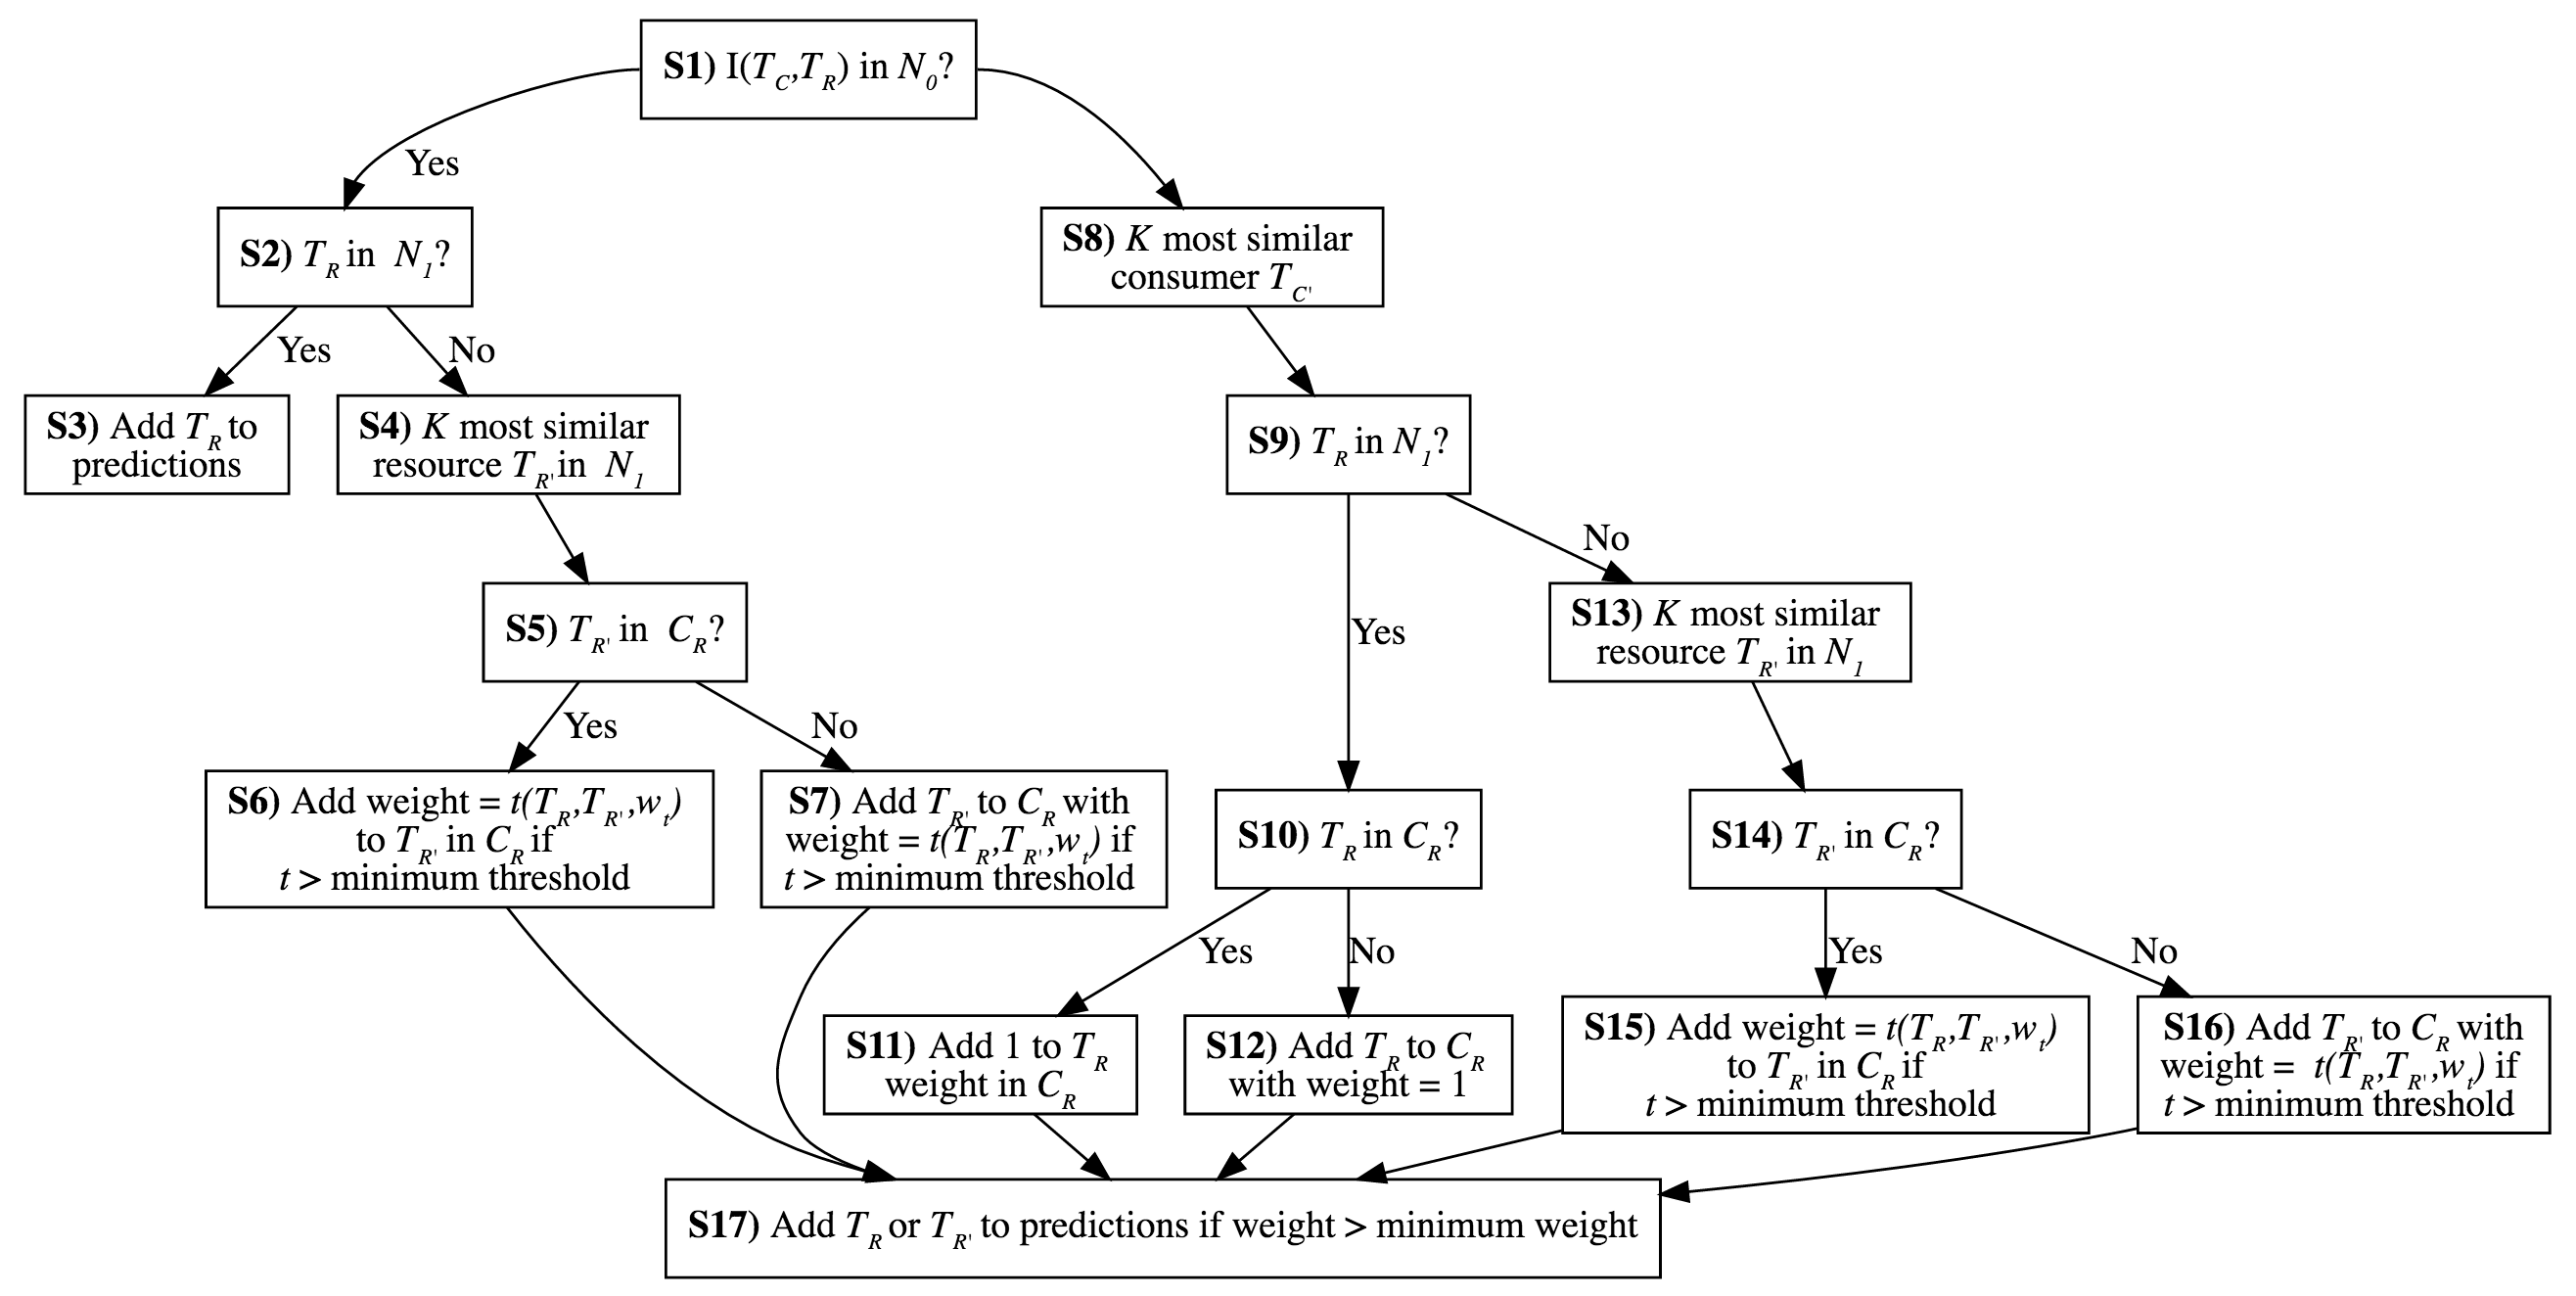
\includegraphics[width=\textwidth]{./figures/ch2-Decision_Diagram.png}
  \caption{Description of 17 logical steps (S1-S17) used by the algorithm to suggest a list of candidate resources ($C_R$) for each consumer taxa ($T_C$) in a set of $N_1$ for which interactions are predicted, using a set of taxa $N_0$ with empirically described interactions. Interactions between consumer and resource taxa are denoted as I($T_C$,$T_R$). $K$ is the number of most similar neighbours selected for the KNN algorithm; $t$ stands for tanimoto in equation 1; $w_t$ is the weight given to sets of resources and consumers in equation 2; the minimum threshold is a value setting the minimal similarity value accepted for taxa to be considered as close neighbours in the KNN algorithm; the weight is the value added to a candidate resource each time it is added to $C_R$; the minimum weight is the minimal weight value accepted for candidate resources to be selected as predicted sources in the algorithm.}
  \label{fig:decision_diag}
\end{figure}


\subsection{Algorithm prediction accuracy}
We used datasets including more than 50 taxa \citep{christian1999, link2002, thompson2004, brose2005, barnes2008, kortsch2015} to assess the prediction accuracy of the algorithm. Testing accuracy of a particular dataset was done by first removing from the catalogue all pairwise interacting taxa originating from that dataset. Accuracy was evaluated using three different statistics:

\begin{enumerate}
 \item $Score_y$ is the fraction of interactions correctly predicted:
     \begin{equation}
         Score_y = \frac{a}{a + c}
     \end{equation}

 \item $Score_{\neg y}$ is the fraction of non-interactions correctly predicted:
     \begin{equation}
       Score_{\neg y}  = \frac{d}{b + d}
     \end{equation}

 \item TSS, The True Skilled Statistics (TSS) evaluated prediction success by considering both true and false predictions, returning a value ranging from 1 (prefect predictions) to -1 (inverted predictions; \cite{allouche2006}):
     \begin{equation}
       TSS = \frac{(ad - bc)}{(a + c)(b + d)}
     \end{equation}
\end{enumerate}

where $a$ is the number of interactions correctly predicted ($i.e.$ true positives), $b$ is the number of non-interactions predicted as interactions ($i.e.$ false positives), $c$ is the number of observed interactions predicted as non-interactions ($i.e.$ false negatives) and $d$ is the number of non-interactions correctly predicted ($i.e.$ true negatives). These three statistics give a different perspective on prediction accuracy, focusing in turn on true interactions and non-interactions, and on both true and false predictions. It is however important to note that false positives and true negatives are solely representative of the datasets used rather than the environment itself. However extensive the datasets may be, unobserved interactions may not necessarily mean a true absence of interaction.

For each statistic, we evaluated prediction accuracy 1) for the complete algorithm, 2) for predictions made through the predictive portion of the algorithm (Steps S4-S16; Figure \ref{fig:decision_diag}) and 3) for the catalogue contribution of the algorithm (Steps S1-S3; Figure \ref{fig:decision_diag}). We evaluated these steps separately in order to partition the relative contribution of the catalogue and of the predictions made using the KNN algorithm to the overall predictive accuracy of the algorithm. Multiple $w_t$ values were also tested to evaluate whether taxa similarity measured as a function of resource/consumer sets or taxonomy contributed more significantly towards increased predictive accuracy. The same was done with multiple $K$ values.

Finally, we evaluated the influence of the comprehensiveness of the catalogue on prediction accuracy. We selected the arctic marine food web from \citet{kortsch2015} as a test. This food web was selected as it is highly detailed taxonomically. Furthermore, once removed from the catalogue, almost 100\% of its taxa still had information available on sets of consumers and resources, which necessary for testing the impact of catalogue comprehensiveness on prediction accuracy. We iteratively and randomly ($n$ = 50 randomizations) removed a percentage of empirical data describing the food web taxa from the catalogue before generating new predictions with the algorithm. We also tested $w_t$ values of 0.5 and 1 to evaluate whether taxonomic similarity could support predictive accuracy in cases when empirical data for species in $N_1$ in the catalogue is unavailable.

% ---------------------------------
% ---------------------------------
%            RESULTS
% ---------------------------------
% ---------------------------------
\section{Results}
    \subsection{Biotic interaction catalogue}
The data compilation process allowed us to build an interaction catalogue composed of $276708$ pairwise interactions (interactions = $72110$; non-interactions = $204598$). A total of 9712 taxa (Superfamily = $15$; Family = $591$; Subfamily = $29$; Tribe = $8$; Genus = $1972$; Species = $7097$) are included in the catalogue, $4159$ of which have data as consumers and $4375$ as resources.

    \subsection{Algorithm predictive accuracy}
The overall predictive accuracy of the algorithm ranges between 80\% to almost 100\% in certain cases (Figure \ref{fig:multi_param}). Both interactions and non-interactions are well predicted by the algorithm. TSS scores are lower than $Score_y$ and $Score_{\neg y}$ due to misclassified interactions and non-interactions. This can also be observed through the effect of varying $K$ values, which increases the number of potential candidate resources for each taxa in the predictive portion of the algorithm. Prediction accuracy increases for interactions, while it decreases for non-interactions, as $K$ values increase.

Similarity being predominantly measured with resource/consumer sets ($w_t$ closer to 0) yielded better predictions than when measured with taxonomy ($w_t$ closer to 1; Figure \ref{fig:multi_param}). Resource/consumer sets therefore appears to serve as a better measure of similarity between taxa for interactions predictions. It is nonetheless interesting to note that although the predictive contribution of the algorithm decreases as $w_t$ increases, an increased mean and decreased variability values for the TSS and $Score_y$ statistics is also observed (Figure \ref{fig:multi_param}). This suggests that while resource/consumer similarity yields higher predictive accuracy, taxonomy better complement the catalogue contribution by predicting interactions not captured through empirical data, effectively increasing the predictive accuracy of the complete algorithm.

The partitioning of the catalogue and predictive portions of the algorithm reveals the importance of the comprehensiveness of the catalogue in prediction accuracy (Figures \ref{fig:multi_param}, \ref{fig:catalog_pred}). As the amount of empirical data available in the catalogue increases so does the overall accuracy of the algorithm (Figures \ref{fig:catalog_pred}). While prediction accuracy of the predictive portion of the algorithm is somewhat lower, it nonetheless supports high prediction efficiency when the catalogue comprehensiveness is lower (Figures \ref{fig:catalog_pred}). Prediction accuracy still remains around 75\% with only 40\% of $N_1$ taxa found in the catalogue (Figures \ref{fig:catalog_pred}). Furthermore, the use of taxonomy for similarity measurements is more efficient when empirical data is scarcer and no different than resource/consumer sets for the complete algorithm when ample data is available (Figures \ref{fig:catalog_pred}).


% Figure 2
\begin{figure}[H]
  \centering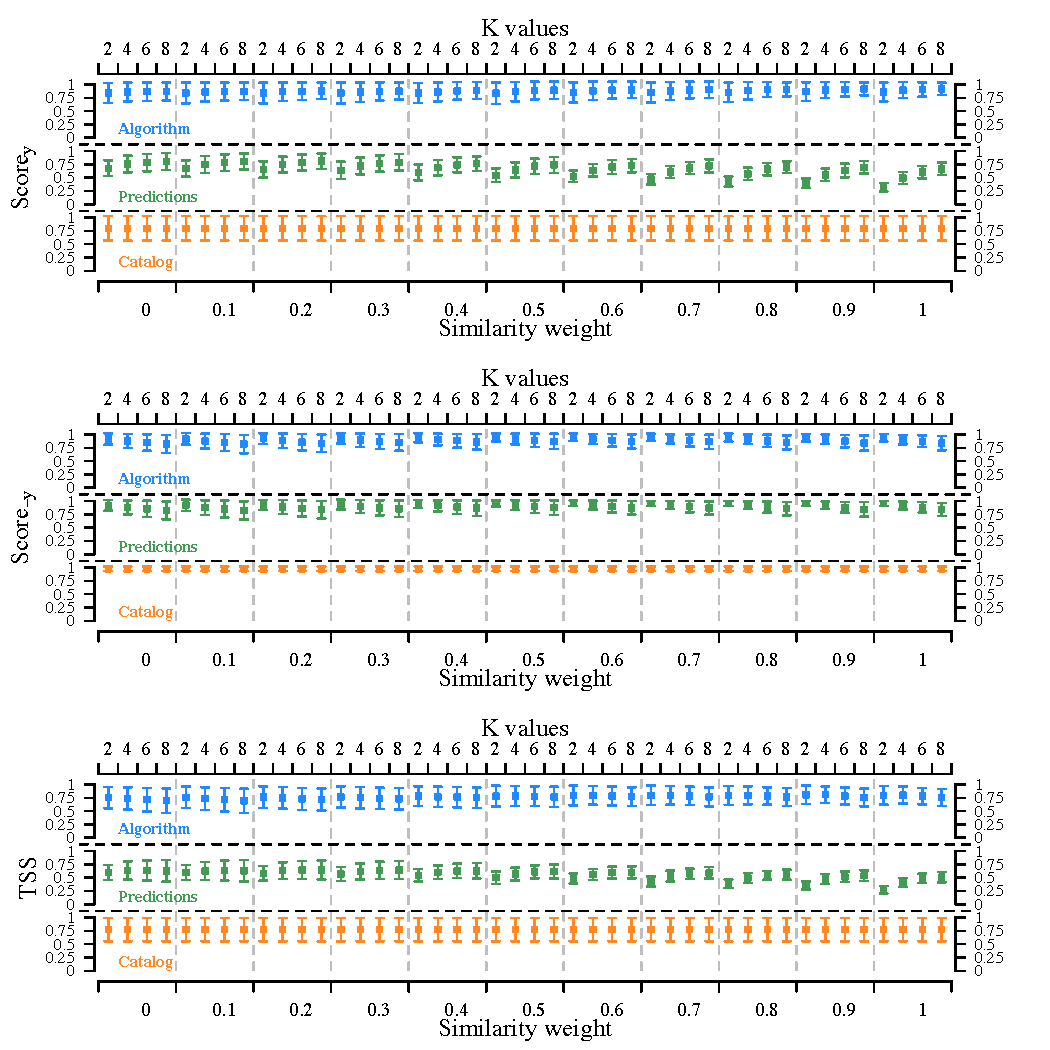
\includegraphics[width=\textwidth, height=12cm]{./figures/ch2-multiple_parameters2.pdf}
  \caption{Representation of the three statistics ($i.e.$ $Score_y$, $Score_{\neg y}$ and TSS) used to evaluate the accuracy of the algorithm as a function of $K$ values tested ($i.e.$ 2, 4, 6 and 8 most similar seighbours, top $x$-axis) and weight for taxonomy (bottom $x$-axis), which varies between 0 and 1. A weight of 0 means that similarity is measured only using set of resources/consumers for each taxa, while a weight of 1 means that similarity is based solely on taxonomy. For each statistic, the topmost panel presents prediction accuracy for the complete algorithm, the middle panel corresponds to predictions made through the predictive portion of the algorithm (Steps S4-S16; Figure \ref{fig:decision_diag}) and the bottom panal presents the catalogue contribution for the algorithm (Steps S1-S3; Figure \ref{fig:decision_diag}). Note that the sum of the predictive and catalogue contributions can be over 100\% as there is overlap between predictions made through both. The 7 datasets used for this analysis contained over 50 taxa \citep{christian1999, link2002, brose2005, thompson2004, barnes2008, kortsch2015}}.
  \label{fig:multi_param}
\end{figure}

% Figure 3
\begin{figure}[H]
  \centering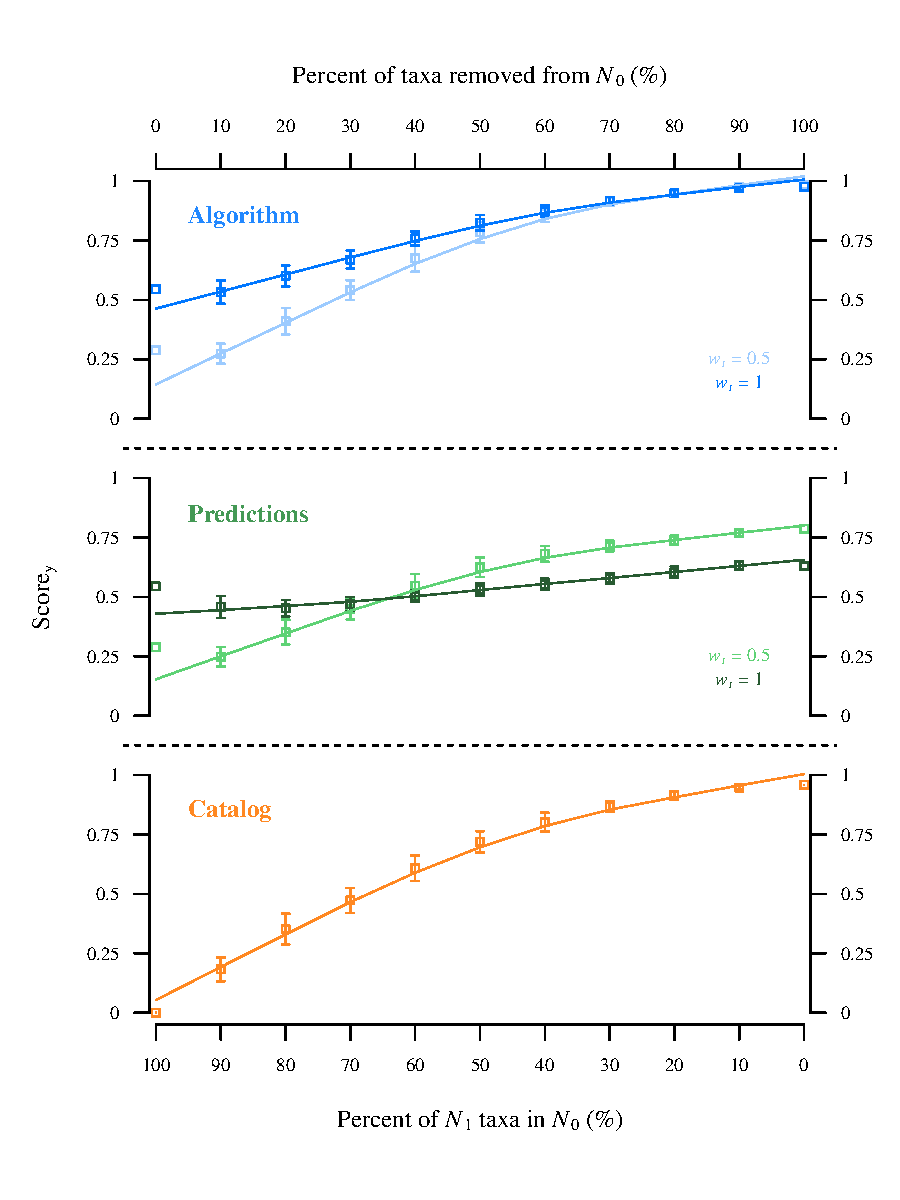
\includegraphics[height=35em]{./figures/ch2-catalog_predictions3.pdf}
  % \caption{Caption on next page.}
  \caption{Representation of $Score_y$ as a function of catalogue comprehensiveness, $i.e.$ the amount of information on sets of consumer and resources available in the catalogue. The sensitivity of the algorithm to data accuracy was evaluation with the arctic food web from \citet{kortsch2015}. This food web was highly detailed taxonomically. Once removed from the catalogue, almost 100\% of its taxa still had information available on sets of consumers and resources, which necessary for testing the impact of catalogue comprehensiveness on prediction accuracy. A random percentage of data available in the catalogue for taxa in the food web ($i.e.$ 0 to 100\%) was iteratively removed ($n$ = 50 randomizations) before generating new predictions with the algorithm. $w_t$ values of 0.5 and 1 were evaluated to verify the usefulness of taxonomy in supporting predictive accuracy. The topmost panel presents prediction accuracy for the complete algorithm, the middle panel corresponds to predictions made through the predictive portion of the algorithm (Steps S4-S16; Figure \ref{fig:decision_diag}) and the bottom panel presents the catalogue contribution for the algorithm (Steps S1-S3; Figure \ref{fig:decision_diag}). Note that the sum of the predictive and catalogue contributions can be over 100\% as there is overlap between predictions made through both.}
  \label{fig:catalog_pred}
\end{figure}


    \subsection{Southern Gulf of St. Lawrence}
As an example, we predict interactions in the southern Gulf of St. Lawrence (SGSL) in eastern Canada. The empirical data and taxa list come from \citet{savenkoff2004}. They present a list of 29 functional groups for a total of 80 taxa presented at least at taxonomical scale of the family. Other coarser functional groups were not used for this example (see Table S1 in Supplementary information (SI) and \citet{savenkoff2004} for a complete description of documented groups).
We used the algorithm to predict interactions between all 80 taxa selected. As their interaction data are reported for functional groups rather than taxa, we then aggregated them back to their original functional groups to compare with interactions presented in \citet{savenkoff2004}. In total, there were empirical data available in the catalogue for 78\% of SGSL taxa (62/80). The algorithm correctly predicted close to 80\% of interactions ($a$ = 135/170) and non-interactions ($d$ = 354/455) extracted from \citet{savenkoff2004}. It also predicted an additional 101 interactions that were not noted in \citet{savenkoff2004} and failed to predict 36 observed interactions that were, resulting in a TSS score of 0.57. A visual comparison of results obtained from the algorithm with interactions noted in \citet{savenkoff2004} is available at Figure \ref{fig:SGSL}. The network presented is centered on the observed and predicted interactions of the capelin (\textit{Mallotus villosus}) and piscivorous small pelagic feeders (e.g. \textit{Scomber scombrus} and \textit{Illex illecebrosus}).

% SGSL accuracy results
% a           b             c           d           TSS         ScoreY1     ScoreY0         FSS
% 135.0000000 101.0000000  35.0000000 354.0000000   0.5721396   0.7941176   0.7780220   0.7824000


% Figure 4
\begin{figure}[H]
  \centering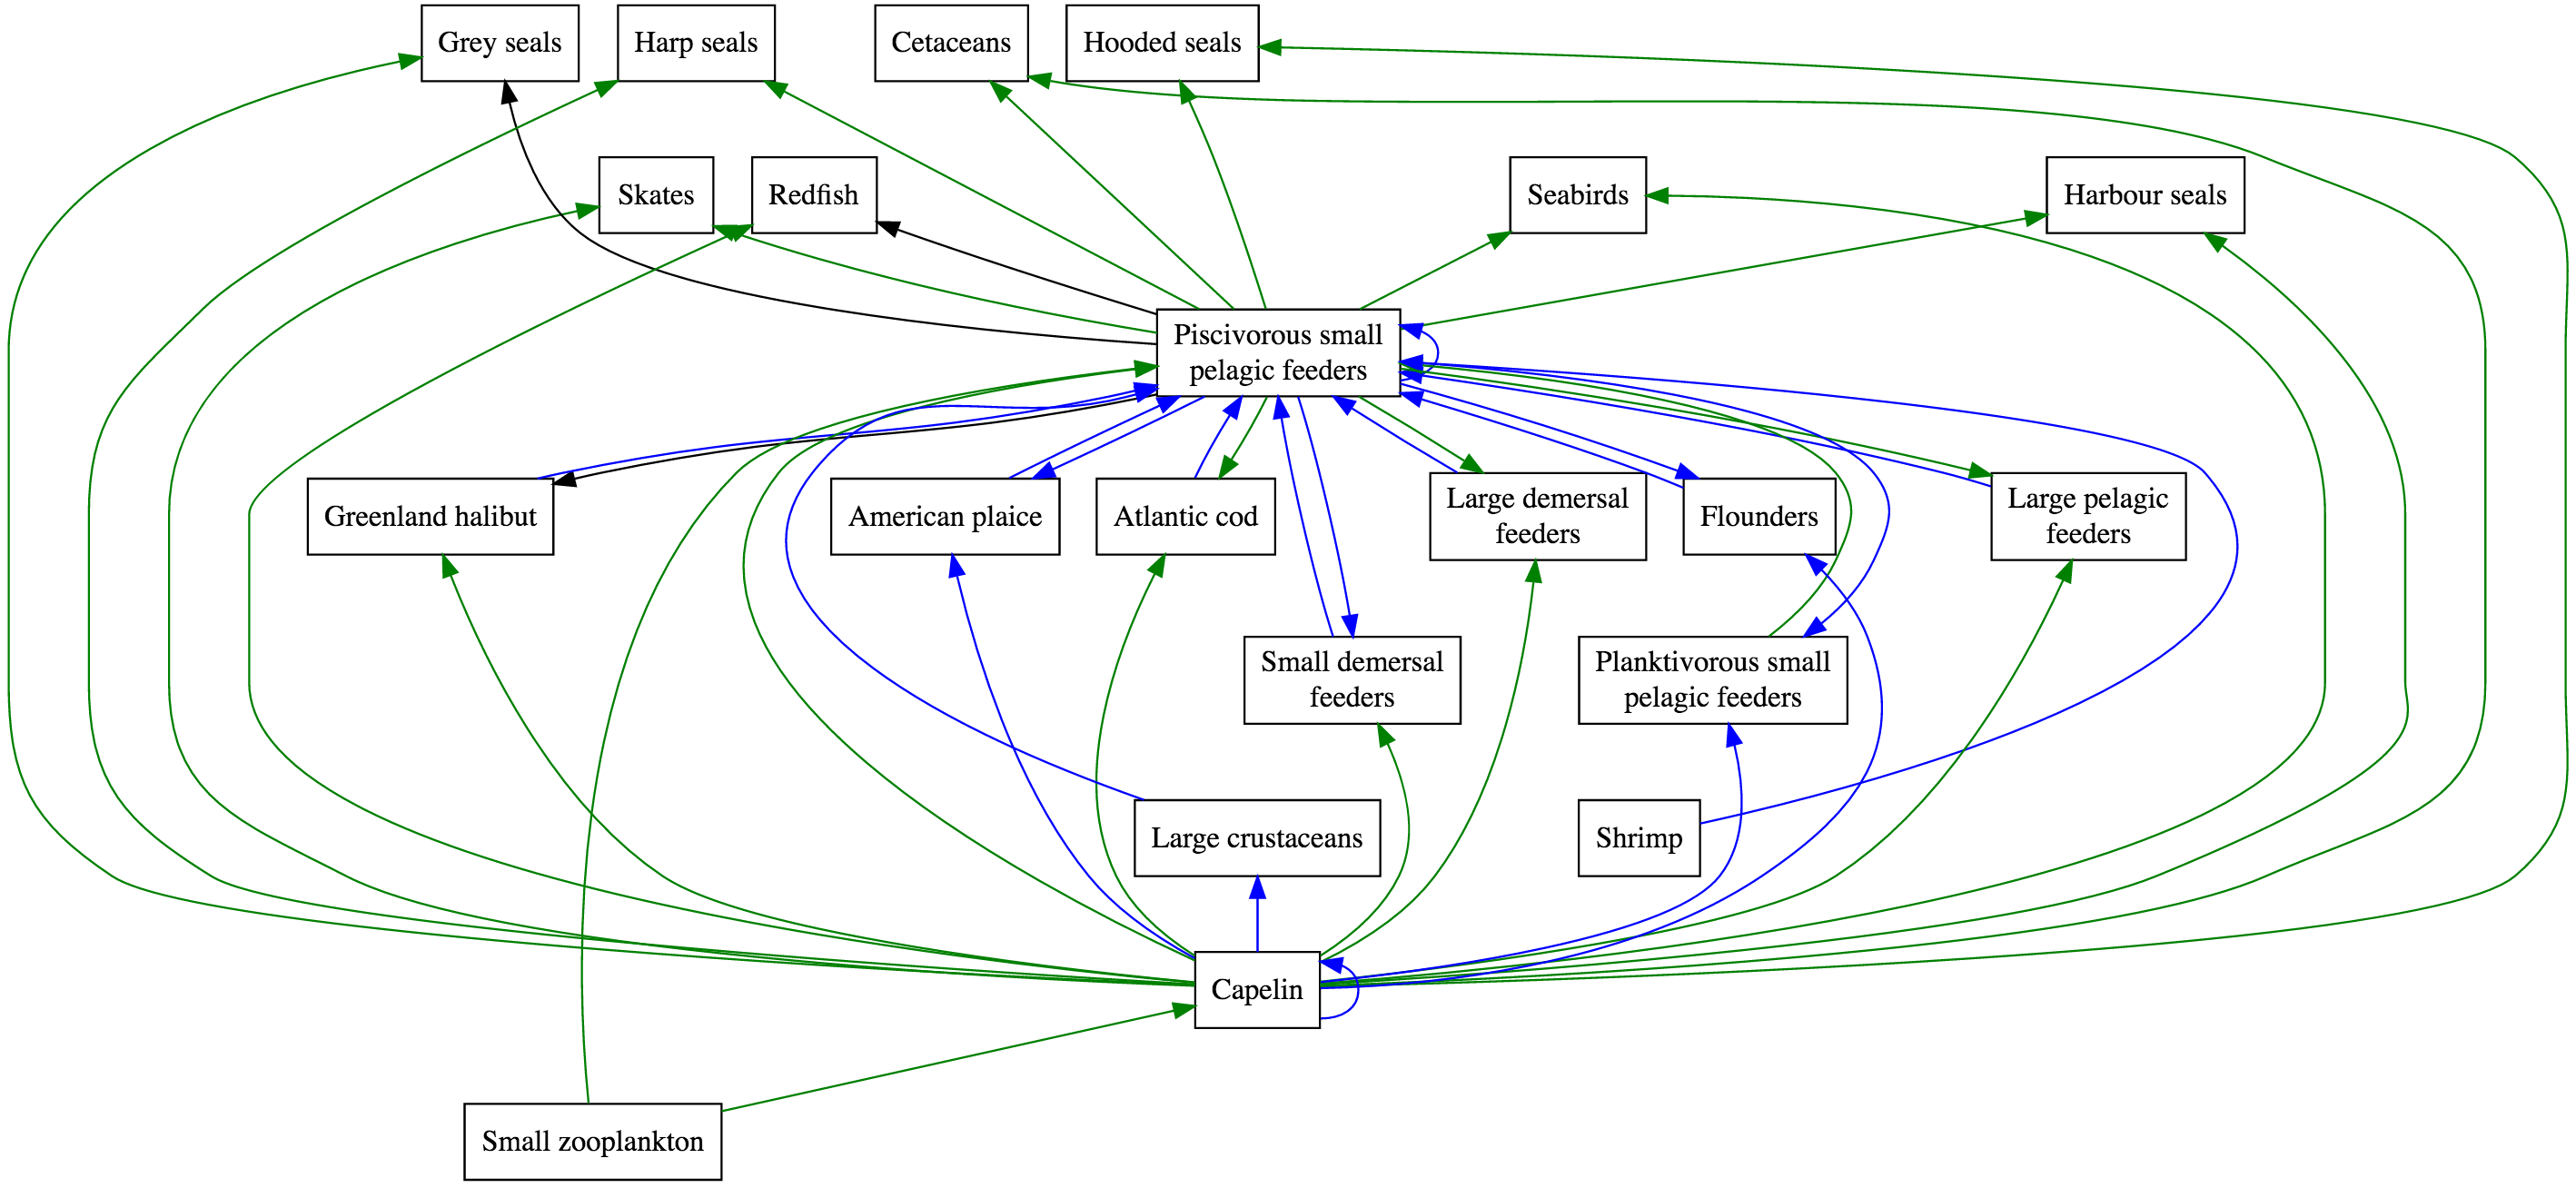
\includegraphics[width=\textwidth]{./figures/ch2-SGSL.png}
  \caption{Example of predicted interactions with the network of the southern Gulf of St. Lawrence \citep{savenkoff2004}, centered around the interactions of the capelin (\textit{Mallotus villosus}) and piscivorous small pelagic feeders (\textit{e.g. Scomber scombrus $and$ Illex illecebrosus}). Edge with colors green were both predicted and observed (26), black were observed only (3) and blue were predicted only (19). Arrows are pointed towards consumers.}
  \label{fig:SGSL}
\end{figure}

% ---------------------------------
% ---------------------------------
%           DISCUSSION
% ---------------------------------
% ---------------------------------
\section{Discussion}
\subsection{Algorithm accuracy}
We show that out of the box interaction inference for a set of taxa with incomplete or unavailable preexisting information can be achieved with high accuracy using a combination of empirical data describing biotic interactions and taxonomic relatedness. Although the efficiency of the algorithm is dependent on the comprehensiveness of the interactions catalogue, taxonomic proximity acts as a complement to increase the number of observed interactions correctly predicted. Taxonomic proximity also supports the efficiency of the algorithm when information gleaned through the catalogue is scarce.

\subsection{Usefulness of taxonomic relatedness}
We found that taxonomy can be highly useful in complementing predictions made using empirical data. Much like the findings from \citet{eklof2016}, evolutionary history provides a significant background from which inferences on network structure can be made. Nonetheless, while evolutionary history plays a significant role in influencing consumer-resource trait matching and food web structure \citep{mouquet2012, rohr2014}, phylogenetic constraints do not necessarily account efficiently for certain traits such as body size \citep{eklof2016}. Complementing our methodology with additional, higher-order information such as functional traits ($e.g.$ metabolism and body size) could thus yield even more efficient results, especially in cases where the catalogue lacks data on taxa for which interactions have to be predicted. Similarly, using phylogenies rather than taxonomy could enhance the resolution at which evolutionary history is considered. This could be achieved through recent efforts to extensively describe all-encompassing phylogenies \citep[e.g.][]{Hedges2015}. Complementing our approach by making it more data dependent could undermine the premise under which this method was built and which constitutes its main strength, $i.e.$ predicting interactions in data deficient environments using readily available data. The flexibility of our methodology would however easily allow for the inclusion of alternate sources of data. Therefore, high-order data such as phylogenies could and should be used in instances where ample data is available, making the use of this methodology broader than simply in instances when data is unavailable.

\subsection{Interactions classification}
That $Score_{y}$ and $Score_{\neg y}$ are inversely proportional means that non-interactions are misclassified as interactions in the process of increasing $Score_y$, consequently decreasing $Score_{\neg y}$. This could either stem from the algorithm poorly predicting non-interactions or from the empirical data itself. Accuracy evaluation assumes that non-interactions from empirical food web are observed data, yet it is usually not the case. Most empirical webs have a strong focus attributed to higher order consumer species and often uneven effort made to thoroughly detail species interactions (\cite{dunne2006}). Furthermore, the methodologies used to obtain consumer-resource data, often relying on gut content analyses, which is efficient at observing interactions, may be inefficient to detect absence of interactions in natural systems (\cite{dunne2006}). This is especially true with our methodology, where we predict interactions between species whose co-occurrence may have been observed in the other ecosystems we are using to predict interactions. Misclassified interactions could thus be real, albeit unobserved through empirical data available.

\subsection{Southern Gulf of St. Lawrence}
The St Lawrence example (Figure \ref{fig:SGSL} and SI) provides adequate material to discuss predictions in greater detail. The algorithm fails to predict 20\% of interactions presented in \citet{savenkoff2004}. Interactions that failed to be predicted were mainly centered on invertebrate species (e.g. polychaetes and mollusks) and taxonomically diverse functional groups described by coarse taxonomic categories (e.g. diatoms) alongside few species in \citet{savenkoff2004} (e.g. piscivorous small pelagic feeders; Table S3). As we focused on the taxa at least at the scale of family, it is likely that their functional groups had a broader range of possible interactions included than what the algorithm could predict using only a few taxa. Furthermore, the efficiency of the algorithm greatly depends on the underlying empirical data that defines the catalogue. If the empirical data used to build the catalogue focuses on higher order consumers, it should come as no surprise that the algorithm would be afflicted by the same limitations.

On the other hand, the algorithm also predicts substantially more interactions than those presented in \citet{savenkoff2004} (Figure \ref{fig:SGSL}; Table S2).  For instance, an important number of additional interactions were predicted for small piscivorous pelagic feeders as consumers (Figure \ref{fig:SGSL}). When considering that these species are typically considered as resources, it should be unsurprising that the broad range of interactions composing the catalogue and from which predictions are made results in new consumer interactions being predicted for those species. An ecological interpretation can therefore be easily provided to explain these additional interactions, such as small piscivorous pelagic feeders consuming cod, likely representing a consumption of cod eggs and/or juveniles. This greatly exemplifies the point we made in the previous section with regards to misclassified interactions being real rather than false positives. The resulting TSS score is therefore greatly diminished by classifying additional interactions as false positives. We therefore believe that the TSS score for the St. Lawrence analysis represents an underestimation of the efficiency of our methodology to predict interactions.

\subsection{Perspectives}

We show that out of the box interaction inference can be achieved with high accuracy using readily available data, suggesting that ecological networks are characterized by a degree of predictability and that this predictive value can be recovered through learning (see \cite{tamaddoni-nezhad2013, gray2015} for other examples). This adds weight to claims that regularities can be observed and predicted in network structure \citep{eklof2016}.

We believe that our methodology offers promising avenues for further applied research and management initiatives. The flexibility of our methodology allows it to take advantage of multiple types of data. Complementing and testing our methodology with additional ecological information such as functional traits and phylogenies would therefore be highly valuable. Interaction strength and species co-occurrence are additional major attributes affecting the probability of observing interactions and the resulting network structure. Interaction strength is instrumental to understanding community dynamics, stability and robustness \citep{laska1998, morales-castilla2015}, while the co-occurrence of species encloses valuable information on interactions and is obviously a pre-requisite for interactions to exist \citep{cazelles2016}. Considering them in our methodology would be highly valuable to correctly assess interactions in a given ecosystem and predict the spatial distribution of interaction networks.

The significance of this approach also extends to other areas of ecological research where gathering data can be highly difficult, such as the reconstruction of interaction networks forming palaeocommunities \citep[e.g.][]{yeakel2013, yeakel2014}. Predicted networks of taxa known to co-occur could be used in hindsight to evaluate the influence of major events such as biodiversity collapse or significant climatic regime shifts on the structure of past ecological communities.

Ultimately, given its high efficiency and simplicity, our methodology could help in promoting the use and the accessibility of food webs and network level descriptors for integrative management initiatives such as cumulative impacts assessments and systematic planning \citep{giakoumi2015, beauchesne2016}, especially for remote locations and frontier areas where empirical data is hard to gather. Network characteristics could be efficiently evaluated and correlated to levels of multiple environmental stressors to assess the vulnerability of ecosystems to global changes \citep{albouy2014}. We believe that the development of such predictive approaches could represent the first much needed steps towards the use of ecological networks in systematic impacts assessments.

\section{Acknowledgements}
We thank the Fond de Recherche Québécois Nature et Technologie (FRQNT) and the Natural Science and Engineering Council of Canada (CRSNG) for financial support. This project is also supported by Québec Océan, the Quebec Centre for Biodiversity Science (QCBS), and the Notre Golfe and CHONeII networks. We also wish to thank K. Cazelles for the help, constructive comments and suggestions. We also thank David Bohan and an anonymous reviewer for their constructive comments and suggestions.



\section{Box 1}

The algorithm follows a series of logical steps to predict resources for all taxa in an arbitrary set of taxa $N_1$ using a set of taxa $N_0$ with empirically described interactions from which we can extract sets of consumers and resources and their taxonomy. In this example, we are predicting interactions for a fictitious $N_1$
 = $\{T_1, T_9, T_{10},T_{11}, T_{12}\}$ using $N_0$ with information on 12 taxa. This catalogue holds information on consumer or resource for 10 taxa and the taxonomy for all 12 taxa in the list.

\begin{singlespace}
    \begin{table}[h!]
      \centering
      \begin{tabular}{cccc}
        \hline
        $N_0$ taxa ID & taxonomy &          resource &             consumer        \\
        \hline
        \hline
        $T_1$ &         $\{a, b, c\}$ &     $\{T_2, T_3, T_{12}\}$ &    $\{T_4\}$         \\
        $T_2$ &         $\{e, f, g\}$ &      &                          $\{T_1, T_5\}$    \\
        $T_3$ &         $\{i, j, k\}$ &      &                          $\{T_5\}$         \\
        $T_4$ &         $\{m, n, o\}$ &     $\{T_1, T_5\}$ &                              \\
        $T_5$ &         $\{a, b, d\}$ &     $\{T_8, T_9\}$ &            $\{T_4\}$         \\
        $T_6$ &         $\{i, q, r\}$ &     $\{T_2, T_8\}$ &            $\{T_4\}$         \\
        $T_7$ &         $\{e, f, h\}$ &      &                          $\{T_1, T_6\}$    \\
        $T_8$ &         $\{s, t, u\}$ &      &                          $\{T_5, T_6\}$    \\
        $T_9$ &         $\{s, t, v\}$ &      &                          $\{T_5\}$         \\
        $T_{10}$ &      $\{i, j, l\}$ &      &                                            \\
        $T_{11}$ &      $\{m, n, p\}$ &      &                                            \\
        $T_{12}$ &      $\{q, r, s\}$ &      &                          $\{T_1\}$         \\
        \hline
      \end{tabular}
    \end{table}
\end{singlespace}

Similarity between all pairs of taxa in $N_0$ is measured for consumer, resource and taxonomic proximity using equation 1. The upper triangular matrix represents similarity measured with taxa sets of resources/consumers, while the lower triangular represents taxonomic similarities. For consumer/resource set similarities, values of 0 mean that similarity equals 0 for both similarity measurements.
\bigskip

    \centerline{$\mbox{tanimoto}(T_Cx, T_Cy)$ / $\mbox{tanimoto}(T_Rx, T_Ry)$ }
\begin{singlespace}
    \begin{table}[h!]
      \centering
      \small
      \begin{tabular}{c|ccccccccccccc}
        & $T_1$ & $T_2$ & $T_3$ & $T_4$ & $T_5$ & $T_6$ & $T_7$ & $T_8$ & $T_9$ & $T_{10}$ & $T_{11}$ & $T_{12}$ \\
        \hline
        $T_1$       & -     & 0     & 0         & 0     & 0/1   & 0.3/1     & 0         & 0         & 0         & 0     & 0     & 0         \\
        $T_2$       & 0     & -     & 0/0.5     & 0     & 0     & 0         & 0/0.3     & 0/0.3     & 0/0.5     & 0     & 0     & 0/0.5     \\
        $T_3$       & 0     & 0     & -         & 0     & 0     & 0         & 0         & 0/0.5     & 0/1       & 0     & 0     & 0         \\
        $T_4$       & 0     & 0     & 0         & -     & 0     & 0         & 0         & 0         & 0         & 0     & 0     & 0         \\
        $T_5$       & 0.5   & 0     & 0         & 0     & -     & 0.3/1     & 0         & 0         & 0         & 0     & 0     & 0         \\
        $T_6$       & 0     & 0     & 0.2       & 0     & 0     & -         & 0         & 0         & 0         & 0     & 0     & 0         \\
        $T_7$       & 0     & 0.5   & 0         & 0     & 0     & 0         & -         & 0/0.3     & 0         & 0     & 0     & 0/0.5     \\
        $T_8$       & 0     & 0     & 0         & 0     & 0     & 0         & 0         & -         & 0         & 0     & 0     & 0         \\
        $T_9$       & 0     & 0     & 0         & 0     & 0     & 0         & 0         & 0.5       & -         & 0     & 0     & 0         \\
        $T_{10}$    & 0     & 0     & 0.5       & 0     & 0     & 0.2       & 0         & 0         & 0         & -     & 0     & 0         \\
        $T_{11}$    & 0     & 0     & 0         & 0.5   & 0     & 0         & 0         & 0         & 0         & 0     & -     & 0         \\
        $T_{12}$    & 0     & 0     & 0         & 0     & 0     & 0.5       & 0         & 0.2       & 0.2       & 0     & 0     & -         \\
      \end{tabular}
    \end{table}
\end{singlespace}
    \centerline{$\mbox{tanimoto}(T_Tx, T_Ty)$}
\bigskip

From these, the algorithm goes through logical steps (Figure \ref{fig:decision_diag}) to identify a candidate resource list $C_R$ for each taxon in $N_1$ using either empirical data directly or $K$ most similar taxa with equation 2. Going through the process for $T_1$, using $K$ = 1 and $w_t$ = 1:
\bigskip

\begin{singlespace}
\begin{table}[h!]
  \centering
  \small
  \begin{tabular}{cl}
      Steps \\
      \hline
      1        &$I(T_1,T_R)$ in $N_0$? \\
      2        &$T_R$ in $N_1$? \\
      4-7      &$T_2$ = no $\rightarrow$ $t(T_2, T_{R'}, w_t)$ = NA   \\
      4-7      &$T_3$ = no $\rightarrow$ $t(T_2, T_{R'}, w_t)$ = $T_{10}$ = 0.5 \\
      3        &$T_{12}$ = yes    \\  \\
      8        &$t(T_1, T_{C'}, w_t)$ = $T_5$ = 0.5            \\
      9        &I($T_5$,$T_R$) in $N_1$? \\
      13-16    &$T_8$ = no $\rightarrow$ $t(T_8, T_{R'}, w_t)$ = $T_9$ = 0.5  \\
      10-12    &$T_9$ = yes   \\
  \end{tabular}
  \begin{tabular}{c|c}
     & \\  \\  \\  \\  \\  \\  \\  \\  \\  \\  \\
  \end{tabular}
  \begin{tabular}{cc}
      Catalogue   & Prediction \\
      \hline \\ \\
      $\{\}$    & $\{\}$            \\
      $\{\}$    & $\{T_{10}\}$      \\
      $\{T_{12}\}$    & $\{T_{10}\}$      \\  \\  \\ \\
      $\{T_{12}\}$    & $\{T_9, T_{10}\}$      \\
      $\{T_9, T_{12}\}$    & $\{T_9, T_{10}\}$      \\
  \end{tabular}
\end{table}
\end{singlespace}
\bigskip

The logical steps allow us to predict a set of resources for $T_1$ = \{$T_9$, $T_{10}$, $T_{12}$\}. Doing it for all taxa in $N_1$ with $w_t$ = 0 and 1 predicts the following networks:
\bigskip

\centerline{\textbf{$w_t$ = 0 \quad \quad \quad \quad \quad $w_t$ = 1} \quad}
    \begin{figure}[H]
    \centering\includegraphics[height = 6cm]{./figures/ch2-example.png}
    \end{figure}


% ---------------------------------
% ---------------------------------
% ---------------------------------
\section{Supporting information}
% ---------------------------------
% ---------------------------------
% ---------------------------------
\begin{singlespace}
\begin{table}[h!]
    \caption{List of functional groups included in the dataset presented in \citet{savenkoff2004} with their taxa composition. Only taxa that were at least at the scale of the family were used to predict interactions. List adapted from \citet{savenkoff2004}.}
    \centering
    \small
    \newcolumntype{b}{>{\hsize=.8\hsize}X}
    \newcolumntype{s}{>{\hsize=.2\hsize}X}
    \begin{tabularx}{1\textwidth}{|s|b|}
        \hline
        Functional group name   & Functional group main taxa composition    \\
        \hline \hline
        Cetaceans                          & $Balaenoptera$ $physalus$, $B.$ $acutorostrata$, $Megaptera$ $novaeangliae$, $Phocoena$ $phocoena$, $Lagenorhynchus$ $acutus$, $L.$ $albirostris$  \\
        \hline
        Harp seals                         & $Pagophilus$ $groenlandicus$   \\
        \hline
        Hooded seals                       & $Cystophora$ $cristata$    \\
        \hline
        Grey seals                         & $Halichoerus$ $grypus$ \\
        \hline
        Harbour seals                      & $Phoca$ $vitulina$ \\
        \hline
        Seabirds                           & $Phalacrocorax$ $carbo$, $P.$ $auritus$, $Larus$ $delawarensis$, $L.$ $argentatus$, $L.$ $marinus$, $Sterna$ $hirundo$, $S.$ $paradisaea$, $Cepphus$ $grylle$, $Oceanodroma$ $leucorhoa$, $Morus$ $bassanus$, $Rissa$ $tridactyla$, $Uria$ $aalge$, $Alca$ $torda$, $Fratercula$ $arctica$ \\
        \hline
        Atlantic cod                       & $Gadus$ $morhua$   \\
        \hline
        Greenland halibut                  & $Reinhardtius$ $hippoglossoides$   \\
        \hline
        American plaice                    & $Hippoglossoides$ $platessoides$   \\
        \hline
        Flounders                          & $Limanda$ $ferruginea$, $Glyptocephalus$ $cynoglossus$, $Pseudopleuronectes$ $americanus$  \\
        \hline
        Skates                             & $Amblyraja$ $radiata$, $Malacoraja$ $senta$, $Leucoraja$ $ocellata$    \\
        \hline
        Redfish                            & $Sebastes$ $mentella$, $S.$ $fasciatus$    \\
        \hline
        Large demersal feeders             & $Urophycis$ $tenuis$, $Melanogrammus$ $aeglefinus$, $Centroscyllium$ $fabricii$, $Anarhichas sp.$, $Cyclopterus$ $lumpus$, $Lycodes sp.$, Macrouridae, Zoarcidae, $Lophius$ $americanus$, $Hippoglossus$ $hippoglossus$    \\
        \hline
        Small demersal feeders             & $Myoxocephalus sp.$, $Tautogolabrus$ $adspersus$, $Zoarces americanus$, large demersal juveniles   \\
        \hline
        Capelin                            & $Mallotus$ $villosus$  \\
        \hline
        Large pelagic feeders              & $Squalus$ $acanthias$, $Pollachius$ $virens$, $Merluccius$ $bilinearis$, $Cetorhinus$ $maximus$    \\
        \hline
        Piscivorous small pelagic feeders  & $Scomber$ $scombrus$, $Illex$ $illecebrosus$, piscivorous myctophids and other mesopelagics, piscivorous large pelagic juveniles   \\
        \hline
        Planktivorous small pelagic feeders& $Clupea$ $harengus$ $harengus$, $Scomberesox$ $saurus$, $Gonatus sp.$, planktivorous myctiphids and other mesopelagics, planktivorous large pelagic juveniles  \\
        \hline
        Shrimp                             & $Argis$ $dentata$, $Eualus$ $macilentus$, $E.$ $gaimardi$, $Pandalus$ $montagui$   \\
        \hline
        Large crustaceans                  & $Chionoecetes$ $opilio$, $Hyas sp.$    \\
        \hline
        Echinoderms                        & $Echinarachnius$ $parma$, $Stronglyocentrotus$ $pallidus$, $Ophiura$ $robusta$ \\
        \hline
  \end{tabularx}

\end{table}

\newpage
\begin{table}[h!]
    \centering
    \small
    \newcolumntype{b}{>{\hsize=.8\hsize}X}
    \newcolumntype{s}{>{\hsize=.2\hsize}X}
    \begin{tabularx}{1\textwidth}{|s|b|}
        \hline
        Functional group name   & Functional group main taxa composition    \\
        \hline \hline
        Molluscs                           & $Mesodesma$ $deauratum$, $Cyrtodaria$ $siliqua$    \\
        \hline
        Polychates                         & $Parexogone$ $hebes$   \\
        \hline
        Small zooplankton                  & $Oithona$ $similis$, $Temora$ $longicornis$, $Pseudocalanus sp.$, $Calanus$ $finmarchicus$, tunicates, meroplankton, heterotrophic protozoa    \\
        \hline
        Phytoplankton                      & $Chaetoceros$ $affinis$, $Chaetoceros sp.$, $Leptocylindrus$ $minimus$, $Thalassiiosira$ $nordenskioldii$, $Thalassiiosira sp.$, $Fragilariopsis sp.$, other diatoms, mixture of autotrophic and mixotrophic organisms including Cryptophytes, dinoflagellates, Prasinophytes and Prymnesiophytes  \\
        \hline
  \end{tabularx}
\end{table}

\newpage
\begin{table}[h!]
  \caption{List of functional groups for which interactions were predicted by the algorithm, but not observed in \citet{savenkoff2004} ($b$).}
    \centering
    \begin{tabular}{|l|l|}
      \hline
        Consumer               & Resource \\
      \hline    \hline
      Skates                              & Skates    \\
      Atlantic cod                        & Skates    \\
      Hooded seals                        & Shrimp    \\
      Piscivorous small pelagic feeders   & Shrimp    \\
      Planktivorous small pelagic feeders & Phytoplankton \\
      Planktivorous small pelagic feeders & Large crustaceans \\
      Hooded seals                        & Large crustaceans \\
      Echinoderms                         & Large crustaceans \\
      Flounders                           & Large crustaceans \\
      Seabirds                            & Large crustaceans \\
      Greenland halibut                   & Large crustaceans \\
      Piscivorous small pelagic feeders   & Large crustaceans \\
      Redfish                             & Large crustaceans \\
      Planktivorous small pelagic feeders & Planktivorous small pelagic feeders   \\
      American plaice                     & Planktivorous small pelagic feeders   \\
      Echinoderms                         & Echinoderms   \\
      Large demersal feeders              & Echinoderms   \\
      Planktivorous small pelagic feeders & Atlantic cod  \\
      American plaice                     & Atlantic cod  \\
      Flounders                           & Atlantic cod  \\
      Greenland halibut                   & Atlantic cod  \\
      Piscivorous small pelagic feeders   & Atlantic cod  \\
      Cetaceans                           & American plaice   \\
      Planktivorous small pelagic feeders & American plaice   \\
      Hooded seals                        & American plaice   \\
      American plaice                     & American plaice   \\
      Flounders                           & American plaice   \\
      Harbour seals                       & American plaice   \\
      Piscivorous small pelagic feeders   & American plaice   \\
      Redfish                             & American plaice   \\
      Large pelagic feeders               & American plaice   \\
      Cetaceans                           & Flounders \\
      Planktivorous small pelagic feeders & Flounders \\
      American plaice                     & Flounders \\
      Flounders                           & Flounders \\
      Piscivorous small pelagic feeders   & Flounders \\
      Redfish                             & Flounders \\
      Large crustaceans                   & Capelin   \\
      Planktivorous small pelagic feeders & Capelin   \\
      Piscivorous small pelagic feeders   & Small demersal feeders    \\
      \hline
  \end{tabular}
\end{table}
\newpage
\begin{table}[h!]
  \centering
  \begin{tabular}{|l|l|}
      \hline
      Consumer               & Resource \\
      \hline    \hline
      Cetaceans                           & Small zooplankton \\
      Large crustaceans                   & Small zooplankton \\
      Large pelagic feeders               & Small zooplankton \\
      Large demersal feeders              & Small zooplankton \\
      Atlantic cod                        & Seabirds  \\
      Seabirds                            & Seabirds  \\
      Large demersal feeders              & Seabirds  \\
      Harbour seals                       & Harbour seals \\
      Skates                              & Greenland halibut \\
      Cetaceans                           & Greenland halibut \\
      Planktivorous small pelagic feeders & Greenland halibut \\
      Atlantic cod                        & Greenland halibut \\
      American plaice                     & Greenland halibut \\
      Flounders                           & Greenland halibut \\
      Small demersal feeders              & Greenland halibut \\
      Harbour seals                       & Greenland halibut \\
      Piscivorous small pelagic feeders   & Greenland halibut \\
      Redfish                             & Greenland halibut \\
      Large pelagic feeders               & Greenland halibut \\
      Planktivorous small pelagic feeders & Piscivorous small pelagic feeders \\
      American plaice                     & Piscivorous small pelagic feeders \\
      Flounders                           & Piscivorous small pelagic feeders \\
      Small demersal feeders              & Piscivorous small pelagic feeders \\
      Piscivorous small pelagic feeders   & Piscivorous small pelagic feeders \\
      Atlantic cod                        & Redfish   \\
      Harp seals                          & Redfish   \\
      Seabirds                            & Redfish   \\
      Redfish                             & Redfish   \\
      Large pelagic feeders               & Redfish   \\
      Skates                              & Large pelagic feeders \\
      Planktivorous small pelagic feeders & Large pelagic feeders \\
      Hooded seals                        & Large pelagic feeders \\
      Atlantic cod                        & Large pelagic feeders \\
      American plaice                     & Large pelagic feeders \\
      Flounders                           & Large pelagic feeders \\
      Small demersal feeders              & Large pelagic feeders \\
      Harp seals                          & Large pelagic feeders \\
      Seabirds                            & Large pelagic feeders \\
      Greenland halibut                   & Large pelagic feeders \\
      Piscivorous small pelagic feeders   & Large pelagic feeders \\
      \hline
    \end{tabular}
\end{table}
\newpage
\begin{table}[h!]
    \centering
    \begin{tabular}{|l|l|}
    \hline
    Consumer               & Resource \\
    \hline    \hline
    Redfish                             & Large pelagic feeders \\
    Large pelagic feeders               & Large pelagic feeders \\
    Large demersal feeders              & Large pelagic feeders \\
    Skates                              & Large demersal feeders    \\
    Cetaceans                           & Large demersal feeders    \\
    Planktivorous small pelagic feeders & Large demersal feeders    \\
    Atlantic cod                        & Large demersal feeders    \\
    American plaice                     & Large demersal feeders    \\
    Flounders                           & Large demersal feeders    \\
    Small demersal feeders              & Large demersal feeders    \\
    Seabirds                            & Large demersal feeders    \\
    Greenland halibut                   & Large demersal feeders    \\
    Piscivorous small pelagic feeders   & Large demersal feeders    \\
    Redfish                             & Large demersal feeders    \\
    Large pelagic feeders               & Large demersal feeders    \\
    Large demersal feeders              & Large demersal feeders    \\
    \hline
\end{tabular}
\end{table}

\newpage
\begin{table}[h!]
  \caption{List of functional groups for which observed interactions in \citet{savenkoff2004} were not predicted by the algorithm ($c$).}
  \centering
  \begin{tabular}{|l|l|}
    \hline
      Consumer               & Resource \\
    \hline  \hline
    Grey seals             & Skates \\
    Seabirds               & Skates \\
    Harbour seals          & Skates \\
    Cetaceans              & Shrimp \\
    Shrimp                 & Phytoplankton  \\
    Mollusks               & Phytoplankton  \\
    Polychaetes            & Phytoplankton  \\
    Grey seals             & Large crustaceans  \\
    Flounders              & Planktivorous small pelagic feeders    \\
    Flounders              & Echinoderms    \\
    Small demersal feeders & Echinoderms    \\
    Grey seals             & American plaice    \\
    Hooded seals           & Flounders  \\
    Harp seals             & Flounders  \\
    Skates                 & Mollusks   \\
    Large crustaceans      & Mollusks   \\
    Atlantic cod           & Mollusks   \\
    American plaice        & Mollusks   \\
    Flounders              & Mollusks   \\
    Small demersal feeders & Mollusks   \\
    Harbour seals          & Mollusks   \\
    Seabirds               & Small zooplankton  \\
    Skates                 & Polychaetes    \\
    Shrimp                 & Polychaetes    \\
    Large crustaceans      & Polychaetes    \\
    Atlantic cod           & Polychaetes    \\
    American plaice        & Polychaetes    \\
    Flounders              & Polychaetes    \\
    Small demersal feeders & Polychaetes    \\
    Polychaetes            & Polychaetes    \\
    Large pelagic feeders  & Polychaetes    \\
    Large demersal feeders & Polychaetes    \\
    Grey seals             & Piscivorous small pelagic feeders  \\
    Greenland halibut      & Piscivorous small pelagic feeders  \\
    Redfish                & Piscivorous small pelagic feeders  \\
    \hline
  \end{tabular}
\end{table}
\end{singlespace}

\chapter{Prédire les interactions biotiques au sein de milieux pauvres en données}
\label{chap3}

\section{Résumé en français du deuxième article}

\subsection{Contexte scientifique}

\subsection{Publication associée}

\subsection{Traduction du résumé de l'article publié}

\section{Title}

Thinking outside the box – predicting biotic interactions in data-poor environments

\section{Authors}

David Beauchesne, Philippe desjardins-proulx2016, Philippe Archambault, Dominique Gravel

% ---------------------------------
% ---------------------------------
%           ABSTRACT
% ---------------------------------
% ---------------------------------
\section{Abstract}
Large networks of ecological interactions, such as food webs, are complex to characterize, be it empirically or theoretically. The former requires exhaustive observations, while the latter generally requires ample data to be validated. We therefore wondered whether readily available data, namely empirically described interactions in a variety of ecosystems, could be combined to predict species interactions in data deficient ecosystems. To test this, we built a biotic interactions catalogue from a collection of 94 empirical food webs, detailed predator-prey interaction databases and interactions from the Global Biotic Interactions (GloBI) database. We used an unsupervised machine learning method to predict interactions between any given set of taxa, given pairwise taxonomic proximity and known consumer and resource sets found in the interaction catalogue. Results suggest that pairwise interactions can be predicted with high accuracy. Although conclusions are seemingly dependent on the comprehensiveness of the catalogue knowledge of taxonomy was found to complement well the catalogue and improve predictions, especially when empirical information available is scarce. Given its high accuracy, this methodology could promote the use of food webs and network level descriptors in certain fields of ecological science in which data is typically hard to gather and in remote and frontier location where empirical data is hard to gather. Network characteristics could then be efficiently evaluated and correlated to levels of environmental stressors in order to improve vulnerability assessments of ecosystems to global changes, opening promising avenues for further research and for management initiatives.
\newline
\textbf{Interactions, machine learning, food webs, K-nearest neighbour, taxonomy, St. Lawrence}

% ---------------------------------
% ---------------------------------
%           INTRODUCTION
% ---------------------------------
% ---------------------------------
\section{Introduction}
Large networks of ecological interactions, such as food webs, are complex to characterize (\cite{polis1991, martinez1992, pascual2006}). Empirical descriptions require exhaustive observations, while theoretical inference generally requires ample data to be validated. For this reason, studies focusing on communities of interacting species remain understudied, even though we acknowledge the importance of considering the reticulated nature of complex networks (\cite{ings2009, tylianakis2008}). When time is of the essence, the long term studies required quickly become impractical and the use of network level approaches relegated to the sideline.

Alternatively, an approach currently gaining in popularity is to predict interactions using proxies such as functional traits, phylogenies and spatial distributions (e.g. \cite{morales-castilla2015, bartomeus2016}). For example, multiple traits can play a significant role in community dynamics and influence the presence and intensity of biotic interactions, like the influence of body size on predator-prey interactions, a literal take on \emph{big fish eats small fish} \citep{cohen2003, brose2006a, gravel2013, seguin2014}. However, the time required to gather the necessary data to apply those methods may still be restrictive, or the data be unavailable altogether, so much so that other methods such as imputation techniques have been developed to fill the gaps in knowledge \citep[e.g.][]{penone2014, schrodt2015}.

We therefore wondered whether more readily available data could be used to infer interactions in data deficient ecosystems. There is an increasing amount of data describing worldwide species interactions, some freely available through the Global Biotic Interactions (GloBI) database \citep{poelen2014}. Similarly, while phylogenies can be challenging to construct and require ample data, a taxonomical description of species is easily accessible through initiatives like the World Register of Marine Species (WoRMS; \cite{bailly2016}). More than simple nomenclature, evolutionary processes are thought to influence and shape consumer-resource relationships \citep{mouquet2012, rohr2014} so that taxonomically related species would be more likely to share similar types of both consumers and resources \citep{eklof2012, morales-castilla2015, gray2015}. Based on that assumption, taxonomy might be a useful surrogate in predicting interactions for species lacking detailed information on their biology, but which have a taxonomically related species for which such information is available.

The objective of this work is thus to combine empirical biotic interactions originating from a variety of ecosystems with taxonomic relatedness to predict interactions in data deficient ecosystems. The concept underlying our methodology is that instead of constraining ourselves to a specific environment, we would look to other environments – outside the box – to glean insights as to the inner workings of an area of interest. As an example, we compare the observed interactions in the southern Gulf of St. Lawrence in Canada (SGSL; \cite{savenkoff2004}) with predictions made using our approach.

% ---------------------------------
% ---------------------------------
%             METHODS
% ---------------------------------
% ---------------------------------
\section{Methods}
The objective of our methodology is to predict the interactions between all pairs of taxa within an arbitrary set $N_1$, using a set of taxa $N_0$ with empirically described interactions from which we can extract pairs of consumers and resources and their taxonomy. We couple the use of empirical data with an unsupervised machine learning method to achieve this.

 \subsection{Biotic interaction catalogue}
We built a biotic interaction catalogue to serve as a set of taxa $N_0$ for with empirically described interactions. The empirical data used to construct the interaction catalogue was gathered in two successive steps. The first consisted of gathering data from a collection of 94 empirical food webs from which we extracted pairwise taxa interactions (see \cite{brose2005, kortsch2015, universityofcanberra2016} for more information). We also used a detailed predator-prey interaction database describing trophic relationships between marine fishes and their prey \citep{barnes2008}. From these datasets, only interactions between taxa at the taxonomic scale of the family or higher were selected for inclusion in the catalogue. Data used came exclusively from marine and coastal ecosystems and encompassed a wide variety of organisms: fungi, algae, parasites, phytoplankton, zooplankton, benthic and pelagic invertebrates, demersal and pelagic fishes, marine birds and marine mammals.

% Modifications to address comments:
As empirical food webs are vastly dominated (96\%) by unobserved or absent interactions ("0", hereafter referred to non-interactions), these datasets yielded a highly skewed distribution of interactions vs non-interactions. To counterbalance this, the second step of data compilation consisted of extracting observed interactions from the Global Biotic Interaction (GloBI) database (\cite{poelen2014}), which describes binary interactions for a wide range of taxa worldwide. We extracted all trophic interactions available on GloBI for species belonging to the families of taxa identified through step 1. Interactions were extracted using the rGloBI package in R (\cite{poelen2015}). As per step 1, only interactions between taxa at the taxonomic scale of the family or higher were retained.

The nomenclature used between datasets and food webs varied substantially. Taxa names thus had to be verified, modified according to the scientific nomenclature and validated. This process was performed using the Taxize package in R \citep{chamberlain2013, chamberlain2014} and manually verified for errors. The same package was used to extract the taxonomy of all taxa for which interactions were obtained in previous steps. The complete R code and data used to build the catalogue is available at \href{https://github.com/david-beauchesne/Interaction_catalog}{https://github.com/david-beauchesne/Interaction\_catalog}.

\subsection{Unsupervised machine learning}
We use the \textit{K}-nearest neighbor (KNN) algorithm \citep{murphy2012} to predict pairwise interactions for a set of taxa $S$. The KNN algorithm predicts missing entries or proposes additional entries by a majority vote based on the $K$ nearest (i.e. most similar) entries (see Box 1 for an example). In this case, taxa are described by a set of resources when considered as a consumer, a set of consumers when considered as a resource and their taxonomy (i.e. kingdom, phylum, class, order, family, genus, species). Similarity between taxa was evaluated using the Tanimoto similarity measure, which compares two vectors $x$ and $y$ with $n = \left\vert{\mathbf{x}}\right\vert = \left\vert{\mathbf{y}}\right\vert$ elements, and is defined as the size of the intersection of two sets divided by their union:

\begin{equation}
\mbox{tanimoto}(\mathbf{x}, \mathbf{y}) = \frac{\left\vert\mathbf{x} \cap \mathbf{y}\right\vert}{\left\vert\mathbf{x} \cup \mathbf{y}\right\vert},
\end{equation}

where \(\cap\) is the intersect and \(\cup\) the union of the vectors. Adding a weighting scheme, we can measure the similarity using two different sets of vectors \(\{\mathbf{x}, \mathbf{y}\}\) and \(\{\mathbf{u}, \mathbf{v}\}\):

\begin{equation}
\label{eq2}
\mbox{tanimoto}_t(x, y, u, v, w_t) = w_t\mbox{tanimoto}(\mathbf{x}, \mathbf{y}) + (1 - w_t)\mbox{tanimoto}(\mathbf{u}, \mathbf{v}),
\end{equation}

where $w_t$ the weight (in $[0;1]$). For our analyses, the first element on the right-hand side of \eqref{eq2} is the Tanimoto similarity measured using the taxonomy of two taxa. The second is the Tanimoto similarity between the sets of resources (or consumers) of the same taxa. When $w_t = 0$ only resource or consumer sets are used to compute similarity, while $w_t = 1$ solely uses taxonomy. This approach to consider the relative contribution of two sets of vectors to the Tanimoto similarity was developed by \citet{desjardins-proulx2016}.

  \subsection{Predicting interactions}
The algorithm was built on a series of logical steps that ultimately predicts a candidate resources list $C_R$ for each taxon in $N_1$ based on empirical data available and the similarity among consumers and among resources (Figure \ref{fig:decision_diag}). For all consumer taxa $T_C$ in $N_1$, the algorithm first verifies, for all resources in resource set $T_R$, if they are found the $N_0$ (Step S1, Figure \ref{fig:decision_diag}). When it does, all $T_R$ taxa that are also in $N_1$ are added as predicted resources for $T_C$ (Steps S2 and S3). This corresponds to what we refer to as the catalogue contribution to resource predictions. In essence, two taxa in $N_1$ that are known to interact through empirical data in the catalogue are automatically assumed to interact in $N_1$.

Otherwise, the algorithm passes to what we refer to as the predictive contribution to resource predictions (Steps S4 to S16), with candidate resources for $T_{Ci}$ (focal taxa for explanation) identified with the KNN algorithm. For each resource in $T_R$ that were not in $N_1$ (Step S2), K most similar resources $T_{R'}$ are identified from $N_1$ (Step S4). If similar resources $T_{R'}$ have a similarity value above a minimal similarity threshold set to 0.3 in our analysis, they are added to $C_R$ as candidate resources. If not, they are automatically discarded (Steps S5 to S7). This minimal threshold is an arbitrary parameter used to avoid predicting resources that have very small and insignificant similarity and hence is very unlikely to share consumers and resources with the taxa it is being compared to.

Then for all consumer taxa $T_C$ in $N_1$, K most similar consumers $T_{C'}$ are identified from $N_0$. This step aims at extracting sets of potential resources $T_R$ from similar types of consumers found in the catalogue (Step S8). Resources $T_R$ are added to candidate resources $C_R$ for $T_{Ci}$ if they are also found in $N_1$ (Steps S10 to S12). Otherwise, Steps S4 to S7 are duplicated to identify potential similar resources for $T_{Ci}$ in $N_1$ from the set of resources $T_R$ of similar consumers $T_{C'}$ (Steps S13 to S16). A simple working example is presented at Box 1. A comprehensive mathematical description of the algorithm and the parameters used is however available through Figure \ref{fig:decision_diag} and the complete R code and data used for the algorithm is available at \href{https://github.com/david-beauchesne/Predict_interactions}{https://github.com/david-beauchesne/Predict\_interactions}.

\subsection{Algorithm prediction accuracy}
We used datasets including more than 50 taxa \citep{christian1999, link2002, thompson2004, brose2005, barnes2008, kortsch2015} to assess the prediction accuracy of the algorithm. Testing accuracy of a particular dataset was done by first removing from the catalogue all pairwise interacting taxa originating from that dataset. Accuracy was evaluated using three different statistics:

\begin{enumerate}
 \item $Score_y$ is the fraction of interactions correctly predicted:
     \begin{equation}
         Score_y = \frac{a}{a + c}
     \end{equation}

 \item $Score_{\neg y}$ is the fraction of non-interactions correctly predicted:
     \begin{equation}
       Score_{\neg y}  = \frac{d}{b + d}
     \end{equation}

 \item TSS, The True Skilled Statistics (TSS) evaluated prediction success by considering both true and false predictions, returning a value ranging from 1 (prefect predictions) to -1 (inverted predictions; \cite{allouche2006}):
     \begin{equation}
       TSS = \frac{(ad - bc)}{(a + c)(b + d)}
     \end{equation}
\end{enumerate}

where $a$ is the number of interactions correctly predicted ($i.e.$ true positives), $b$ is the number of non-interactions predicted as interactions ($i.e.$ false positives), $c$ is the number of observed interactions predicted as non-interactions ($i.e.$ false negatives) and $d$ is the number of non-interactions correctly predicted ($i.e.$ true negatives). These three statistics give a different perspective on prediction accuracy, focusing in turn on true interactions and non-interactions, and on both true and false predictions. It is however important to note that false positives and true negatives are solely representative of the datasets used rather than the environment itself. However extensive the datasets may be, unobserved interactions may not necessarily mean a true absence of interaction.

For each statistic, we evaluated prediction accuracy 1) for the complete algorithm, 2) for predictions made through the predictive portion of the algorithm (Steps S4-S16; Figure \ref{fig:decision_diag}) and 3) for the catalogue contribution of the algorithm (Steps S1-S3; Figure \ref{fig:decision_diag}). We evaluated these steps separately in order to partition the relative contribution of the catalogue and of the predictions made using the KNN algorithm to the overall predictive accuracy of the algorithm. Multiple $w_t$ values were also tested to evaluate whether taxa similarity measured as a function of resource/consumer sets or taxonomy contributed more significantly towards increased predictive accuracy. The same was done with multiple $K$ values.

Finally, we evaluated the influence of the comprehensiveness of the catalogue on prediction accuracy. We selected the arctic marine food web from \citet{kortsch2015} as a test. This food web was selected as it is highly detailed taxonomically. Furthermore, once removed from the catalogue, almost 100\% of its taxa still had information available on sets of consumers and resources, which necessary for testing the impact of catalogue comprehensiveness on prediction accuracy. We iteratively and randomly ($n$ = 50 randomizations) removed a percentage of empirical data describing the food web taxa from the catalogue before generating new predictions with the algorithm. We also tested $w_t$ values of 0.5 and 1 to evaluate whether taxonomic similarity could support predictive accuracy in cases when empirical data for species in $N_1$ in the catalogue is unavailable.

% ---------------------------------
% ---------------------------------
%            RESULTS
% ---------------------------------
% ---------------------------------
\section{Results}
    \subsection{Biotic interaction catalogue}
The data compilation process allowed us to build an interaction catalogue composed of $276708$ pairwise interactions (interactions = $72110$; non-interactions = $204598$). A total of 9712 taxa (Superfamily = $15$; Family = $591$; Subfamily = $29$; Tribe = $8$; Genus = $1972$; Species = $7097$) are included in the catalogue, $4159$ of which have data as consumers and $4375$ as resources.

    \subsection{Algorithm predictive accuracy}
The overall predictive accuracy of the algorithm ranges between 80\% to almost 100\% in certain cases (Figure \ref{fig:multi_param}). Both interactions and non-interactions are well predicted by the algorithm. TSS scores are lower than $Score_y$ and $Score_{\neg y}$ due to misclassified interactions and non-interactions. This can also be observed through the effect of varying $K$ values, which increases the number of potential candidate resources for each taxa in the predictive portion of the algorithm. Prediction accuracy increases for interactions, while it decreases for non-interactions, as $K$ values increase.

Similarity being predominantly measured with resource/consumer sets ($w_t$ closer to 0) yielded better predictions than when measured with taxonomy ($w_t$ closer to 1; Figure \ref{fig:multi_param}). Resource/consumer sets therefore appears to serve as a better measure of similarity between taxa for interactions predictions. It is nonetheless interesting to note that although the predictive contribution of the algorithm decreases as $w_t$ increases, an increased mean and decreased variability values for the TSS and $Score_y$ statistics is also observed (Figure \ref{fig:multi_param}). This suggests that while resource/consumer similarity yields higher predictive accuracy, taxonomy better complement the catalogue contribution by predicting interactions not captured through empirical data, effectively increasing the predictive accuracy of the complete algorithm.

The partitioning of the catalogue and predictive portions of the algorithm reveals the importance of the comprehensiveness of the catalogue in prediction accuracy (Figures \ref{fig:multi_param}, \ref{fig:catalog_pred}). As the amount of empirical data available in the catalogue increases so does the overall accuracy of the algorithm (Figures \ref{fig:catalog_pred}). While prediction accuracy of the predictive portion of the algorithm is somewhat lower, it nonetheless supports high prediction efficiency when the catalogue comprehensiveness is lower (Figures \ref{fig:catalog_pred}). Prediction accuracy still remains around 75\% with only 40\% of $N_1$ taxa found in the catalogue (Figures \ref{fig:catalog_pred}). Furthermore, the use of taxonomy for similarity measurements is more efficient when empirical data is scarcer and no different than resource/consumer sets for the complete algorithm when ample data is available (Figures \ref{fig:catalog_pred}).

    \subsection{Southern Gulf of St. Lawrence}
As an example, we predict interactions in the southern Gulf of St. Lawrence (SGSL) in eastern Canada. The empirical data and taxa list come from \citet{savenkoff2004}. They present a list of 29 functional groups for a total of 80 taxa presented at least at taxonomical scale of the family. Other coarser functional groups were not used for this example (see Table S1 in Supplementary information (SI) and \citet{savenkoff2004} for a complete description of documented groups).
We used the algorithm to predict interactions between all 80 taxa selected. As their interaction data are reported for functional groups rather than taxa, we then aggregated them back to their original functional groups to compare with interactions presented in \citet{savenkoff2004}. In total, there were empirical data available in the catalogue for 78\% of SGSL taxa (62/80). The algorithm correctly predicted close to 80\% of interactions ($a$ = 135/170) and non-interactions ($d$ = 354/455) extracted from \citet{savenkoff2004}. It also predicted an additional 101 interactions that were not noted in \citet{savenkoff2004} and failed to predict 36 observed interactions that were, resulting in a TSS score of 0.57. A visual comparison of results obtained from the algorithm with interactions noted in \citet{savenkoff2004} is available at Figure \ref{fig:SGSL}. The network presented is centered on the observed and predicted interactions of the capelin (\textit{Mallotus villosus}) and piscivorous small pelagic feeders (e.g. \textit{Scomber scombrus} and \textit{Illex illecebrosus}).

% SGSL accuracy results
% a           b             c           d           TSS         ScoreY1     ScoreY0         FSS
% 135.0000000 101.0000000  35.0000000 354.0000000   0.5721396   0.7941176   0.7780220   0.7824000

% ---------------------------------
% ---------------------------------
%           DISCUSSION
% ---------------------------------
% ---------------------------------
\section{Discussion}
\subsection{Algorithm accuracy}
We show that out of the box interaction inference for a set of taxa with incomplete or unavailable preexisting information can be achieved with high accuracy using a combination of empirical data describing biotic interactions and taxonomic relatedness. Although the efficiency of the algorithm is dependent on the comprehensiveness of the interactions catalogue, taxonomic proximity acts as a complement to increase the number of observed interactions correctly predicted. Taxonomic proximity also supports the efficiency of the algorithm when information gleaned through the catalogue is scarce.

\subsection{Usefulness of taxonomic relatedness}
We found that taxonomy can be highly useful in complementing predictions made using empirical data. Much like the findings from \citet{eklof2016}, evolutionary history provides a significant background from which inferences on network structure can be made. Nonetheless, while evolutionary history plays a significant role in influencing consumer-resource trait matching and food web structure \citep{mouquet2012, rohr2014}, phylogenetic constraints do not necessarily account efficiently for certain traits such as body size \citep{eklof2016}. Complementing our methodology with additional, higher-order information such as functional traits ($e.g.$ metabolism and body size) could thus yield even more efficient results, especially in cases where the catalogue lacks data on taxa for which interactions have to be predicted. Similarly, using phylogenies rather than taxonomy could enhance the resolution at which evolutionary history is considered. This could be achieved through recent efforts to extensively describe all-encompassing phylogenies \citep[e.g.][]{Hedges2015}. Complementing our approach by making it more data dependent could undermine the premise under which this method was built and which constitutes its main strength, $i.e.$ predicting interactions in data deficient environments using readily available data. The flexibility of our methodology would however easily allow for the inclusion of alternate sources of data. Therefore, high-order data such as phylogenies could and should be used in instances where ample data is available, making the use of this methodology broader than simply in instances when data is unavailable.

\subsection{Interactions classification}
That $Score_{y}$ and $Score_{\neg y}$ are inversely proportional means that non-interactions are misclassified as interactions in the process of increasing $Score_y$, consequently decreasing $Score_{\neg y}$. This could either stem from the algorithm poorly predicting non-interactions or from the empirical data itself. Accuracy evaluation assumes that non-interactions from empirical food web are observed data, yet it is usually not the case. Most empirical webs have a strong focus attributed to higher order consumer species and often uneven effort made to thoroughly detail species interactions (\cite{dunne2006}). Furthermore, the methodologies used to obtain consumer-resource data, often relying on gut content analyses, which is efficient at observing interactions, may be inefficient to detect absence of interactions in natural systems (\cite{dunne2006}). This is especially true with our methodology, where we predict interactions between species whose co-occurrence may have been observed in the other ecosystems we are using to predict interactions. Misclassified interactions could thus be real, albeit unobserved through empirical data available.

\subsection{Southern Gulf of St. Lawrence}
The St Lawrence example (Figure \ref{fig:SGSL} and SI) provides adequate material to discuss predictions in greater detail. The algorithm fails to predict 20\% of interactions presented in \citet{savenkoff2004}. Interactions that failed to be predicted were mainly centered on invertebrate species (e.g. polychaetes and mollusks) and taxonomically diverse functional groups described by coarse taxonomic categories (e.g. diatoms) alongside few species in \citet{savenkoff2004} (e.g. piscivorous small pelagic feeders; Table S3). As we focused on the taxa at least at the scale of family, it is likely that their functional groups had a broader range of possible interactions included than what the algorithm could predict using only a few taxa. Furthermore, the efficiency of the algorithm greatly depends on the underlying empirical data that defines the catalogue. If the empirical data used to build the catalogue focuses on higher order consumers, it should come as no surprise that the algorithm would be afflicted by the same limitations.

On the other hand, the algorithm also predicts substantially more interactions than those presented in \citet{savenkoff2004} (Figure \ref{fig:SGSL}; Table S2).  For instance, an important number of additional interactions were predicted for small piscivorous pelagic feeders as consumers (Figure \ref{fig:SGSL}). When considering that these species are typically considered as resources, it should be unsurprising that the broad range of interactions composing the catalogue and from which predictions are made results in new consumer interactions being predicted for those species. An ecological interpretation can therefore be easily provided to explain these additional interactions, such as small piscivorous pelagic feeders consuming cod, likely representing a consumption of cod eggs and/or juveniles. This greatly exemplifies the point we made in the previous section with regards to misclassified interactions being real rather than false positives. The resulting TSS score is therefore greatly diminished by classifying additional interactions as false positives. We therefore believe that the TSS score for the St. Lawrence analysis represents an underestimation of the efficiency of our methodology to predict interactions.

\subsection{Perspectives}

We show that out of the box interaction inference can be achieved with high accuracy using readily available data, suggesting that ecological networks are characterized by a degree of predictability and that this predictive value can be recovered through learning (see \cite{tamaddoni-nezhad2013, gray2015} for other examples). This adds weight to claims that regularities can be observed and predicted in network structure \citep{eklof2016}.

We believe that our methodology offers promising avenues for further applied research and management initiatives. The flexibility of our methodology allows it to take advantage of multiple types of data. Complementing and testing our methodology with additional ecological information such as functional traits and phylogenies would therefore be highly valuable. Interaction strength and species co-occurrence are additional major attributes affecting the probability of observing interactions and the resulting network structure. Interaction strength is instrumental to understanding community dynamics, stability and robustness \citep{laska1998, morales-castilla2015}, while the co-occurrence of species encloses valuable information on interactions and is obviously a pre-requisite for interactions to exist \citep{cazelles2016}. Considering them in our methodology would be highly valuable to correctly assess interactions in a given ecosystem and predict the spatial distribution of interaction networks.

The significance of this approach also extends to other areas of ecological research where gathering data can be highly difficult, such as the reconstruction of interaction networks forming palaeocommunities \citep[e.g.][]{yeakel2013, yeakel2014}. Predicted networks of taxa known to co-occur could be used in hindsight to evaluate the influence of major events such as biodiversity collapse or significant climatic regime shifts on the structure of past ecological communities.

Ultimately, given its high efficiency and simplicity, our methodology could help in promoting the use and the accessibility of food webs and network level descriptors for integrative management initiatives such as cumulative impacts assessments and systematic planning \citep{giakoumi2015, beauchesne2016}, especially for remote locations and frontier areas where empirical data is hard to gather. Network characteristics could be efficiently evaluated and correlated to levels of multiple environmental stressors to assess the vulnerability of ecosystems to global changes \citep{albouy2014}. We believe that the development of such predictive approaches could represent the first much needed steps towards the use of ecological networks in systematic impacts assessments.

\section{Acknowledgements}
We thank the Fond de Recherche Québécois Nature et Technologie (FRQNT) and the Natural Science and Engineering Council of Canada (CRSNG) for financial support. This project is also supported by Québec Océan, the Quebec Centre for Biodiversity Science (QCBS), and the Notre Golfe and CHONeII networks. We also wish to thank K. Cazelles for the help, constructive comments and suggestions. We also thank David Bohan and an anonymous reviewer for their constructive comments and suggestions.



\newpage
\subsection{Box 1}

The algorithm follows a series of logical steps to predict resources for all taxa in an arbitrary set of taxa $N_1$ using a set of taxa $N_0$ with empirically described interactions from which we can extract sets of consumers and resources and their taxonomy. In this example, we are predicting interactions for a fictitious $N_1$
 = $\{T_1, T_9, T_{10},T_{11}, T_{12}\}$ using $N_0$ with information on 12 taxa. This catalogue holds information on consumer or resource for 10 taxa and the taxonomy for all 12 taxa in the list.

    \begin{table}[h!]
      \centering
      \begin{tabular}{cccc}
        \hline
        $N_0$ taxa ID & taxonomy &          resource &             consumer        \\
        \hline
        \hline
        $T_1$ &         $\{a, b, c\}$ &     $\{T_2, T_3, T_{12}\}$ &    $\{T_4\}$         \\
        $T_2$ &         $\{e, f, g\}$ &      &                          $\{T_1, T_5\}$    \\
        $T_3$ &         $\{i, j, k\}$ &      &                          $\{T_5\}$         \\
        $T_4$ &         $\{m, n, o\}$ &     $\{T_1, T_5\}$ &                              \\
        $T_5$ &         $\{a, b, d\}$ &     $\{T_8, T_9\}$ &            $\{T_4\}$         \\
        $T_6$ &         $\{i, q, r\}$ &     $\{T_2, T_8\}$ &            $\{T_4\}$         \\
        $T_7$ &         $\{e, f, h\}$ &      &                          $\{T_1, T_6\}$    \\
        $T_8$ &         $\{s, t, u\}$ &      &                          $\{T_5, T_6\}$    \\
        $T_9$ &         $\{s, t, v\}$ &      &                          $\{T_5\}$         \\
        $T_{10}$ &      $\{i, j, l\}$ &      &                                            \\
        $T_{11}$ &      $\{m, n, p\}$ &      &                                            \\
        $T_{12}$ &      $\{q, r, s\}$ &      &                          $\{T_1\}$         \\
        \hline
      \end{tabular}
    \end{table}

Similarity between all pairs of taxa in $N_0$ is measured for consumer, resource and taxonomic proximity using equation 1. The upper triangular matrix represents similarity measured with taxa sets of resources/consumers, while the lower triangular represents taxonomic similarities. For consumer/resource set similarities, values of 0 mean that similarity equals 0 for both similarity measurements.
\bigskip

    \centerline{$\mbox{tanimoto}(T_Cx, T_Cy)$ / $\mbox{tanimoto}(T_Rx, T_Ry)$ }

    \begin{table}[h!]
      \centering
      \small
      \begin{tabular}{c|ccccccccccccc}
        & $T_1$ & $T_2$ & $T_3$ & $T_4$ & $T_5$ & $T_6$ & $T_7$ & $T_8$ & $T_9$ & $T_{10}$ & $T_{11}$ & $T_{12}$ \\
        \hline
        $T_1$       & -     & 0     & 0         & 0     & 0/1   & 0.3/1     & 0         & 0         & 0         & 0     & 0     & 0         \\
        $T_2$       & 0     & -     & 0/0.5     & 0     & 0     & 0         & 0/0.3     & 0/0.3     & 0/0.5     & 0     & 0     & 0/0.5     \\
        $T_3$       & 0     & 0     & -         & 0     & 0     & 0         & 0         & 0/0.5     & 0/1       & 0     & 0     & 0         \\
        $T_4$       & 0     & 0     & 0         & -     & 0     & 0         & 0         & 0         & 0         & 0     & 0     & 0         \\
        $T_5$       & 0.5   & 0     & 0         & 0     & -     & 0.3/1     & 0         & 0         & 0         & 0     & 0     & 0         \\
        $T_6$       & 0     & 0     & 0.2       & 0     & 0     & -         & 0         & 0         & 0         & 0     & 0     & 0         \\
        $T_7$       & 0     & 0.5   & 0         & 0     & 0     & 0         & -         & 0/0.3     & 0         & 0     & 0     & 0/0.5     \\
        $T_8$       & 0     & 0     & 0         & 0     & 0     & 0         & 0         & -         & 0         & 0     & 0     & 0         \\
        $T_9$       & 0     & 0     & 0         & 0     & 0     & 0         & 0         & 0.5       & -         & 0     & 0     & 0         \\
        $T_{10}$    & 0     & 0     & 0.5       & 0     & 0     & 0.2       & 0         & 0         & 0         & -     & 0     & 0         \\
        $T_{11}$    & 0     & 0     & 0         & 0.5   & 0     & 0         & 0         & 0         & 0         & 0     & -     & 0         \\
        $T_{12}$    & 0     & 0     & 0         & 0     & 0     & 0.5       & 0         & 0.2       & 0.2       & 0     & 0     & -         \\
      \end{tabular}
    \end{table}

    \centerline{$\mbox{tanimoto}(T_Tx, T_Ty)$}
\bigskip

From these, the algorithm goes through logical steps (Figure \ref{fig:decision_diag}) to identify a candidate resource list $C_R$ for each taxon in $N_1$ using either empirical data directly or $K$ most similar taxa with equation 2. Going through the process for $T_1$, using $K$ = 1 and $w_t$ = 1:
\bigskip

\begin{table}[h!]
  \centering
  \small
  \begin{tabular}{cl}
      Steps \\
      \hline
      1        &$I(T_1,T_R)$ in $N_0$? \\
      2        &$T_R$ in $N_1$? \\
      4-7      &$T_2$ = no $\rightarrow$ $t(T_2, T_{R'}, w_t)$ = NA   \\
      4-7      &$T_3$ = no $\rightarrow$ $t(T_2, T_{R'}, w_t)$ = $T_{10}$ = 0.5 \\
      3        &$T_{12}$ = yes    \\  \\
      8        &$t(T_1, T_{C'}, w_t)$ = $T_5$ = 0.5            \\
      9        &I($T_5$,$T_R$) in $N_1$? \\
      13-16    &$T_8$ = no $\rightarrow$ $t(T_8, T_{R'}, w_t)$ = $T_9$ = 0.5  \\
      10-12    &$T_9$ = yes   \\
  \end{tabular}
  \begin{tabular}{c|c}
     & \\  \\  \\  \\  \\  \\  \\  \\  \\  \\  \\
  \end{tabular}
  \begin{tabular}{cc}
      Catalogue   & Prediction \\
      \hline \\ \\
      $\{\}$    & $\{\}$            \\
      $\{\}$    & $\{T_{10}\}$      \\
      $\{T_{12}\}$    & $\{T_{10}\}$      \\  \\  \\ \\
      $\{T_{12}\}$    & $\{T_9, T_{10}\}$      \\
      $\{T_9, T_{12}\}$    & $\{T_9, T_{10}\}$      \\
  \end{tabular}
\end{table}
\bigskip

The logical steps allow us to predict a set of resources for $T_1$ = \{$T_9$, $T_{10}$, $T_{12}$\}. Doing it for all taxa in $N_1$ with $w_t$ = 0 and 1 predicts the following networks:
\bigskip

\centerline{\textbf{$w_t$ = 0 \quad \quad \quad \quad \quad $w_t$ = 1} \quad}
    \begin{figure}[h!]
    \centering\includegraphics[height = 6cm]{./chapitre3/figures/example.png}
    \end{figure}

% Example finish

%Figure 1
\newpage
\subsection{Figures}
    \begin{figure}[h]
      \centering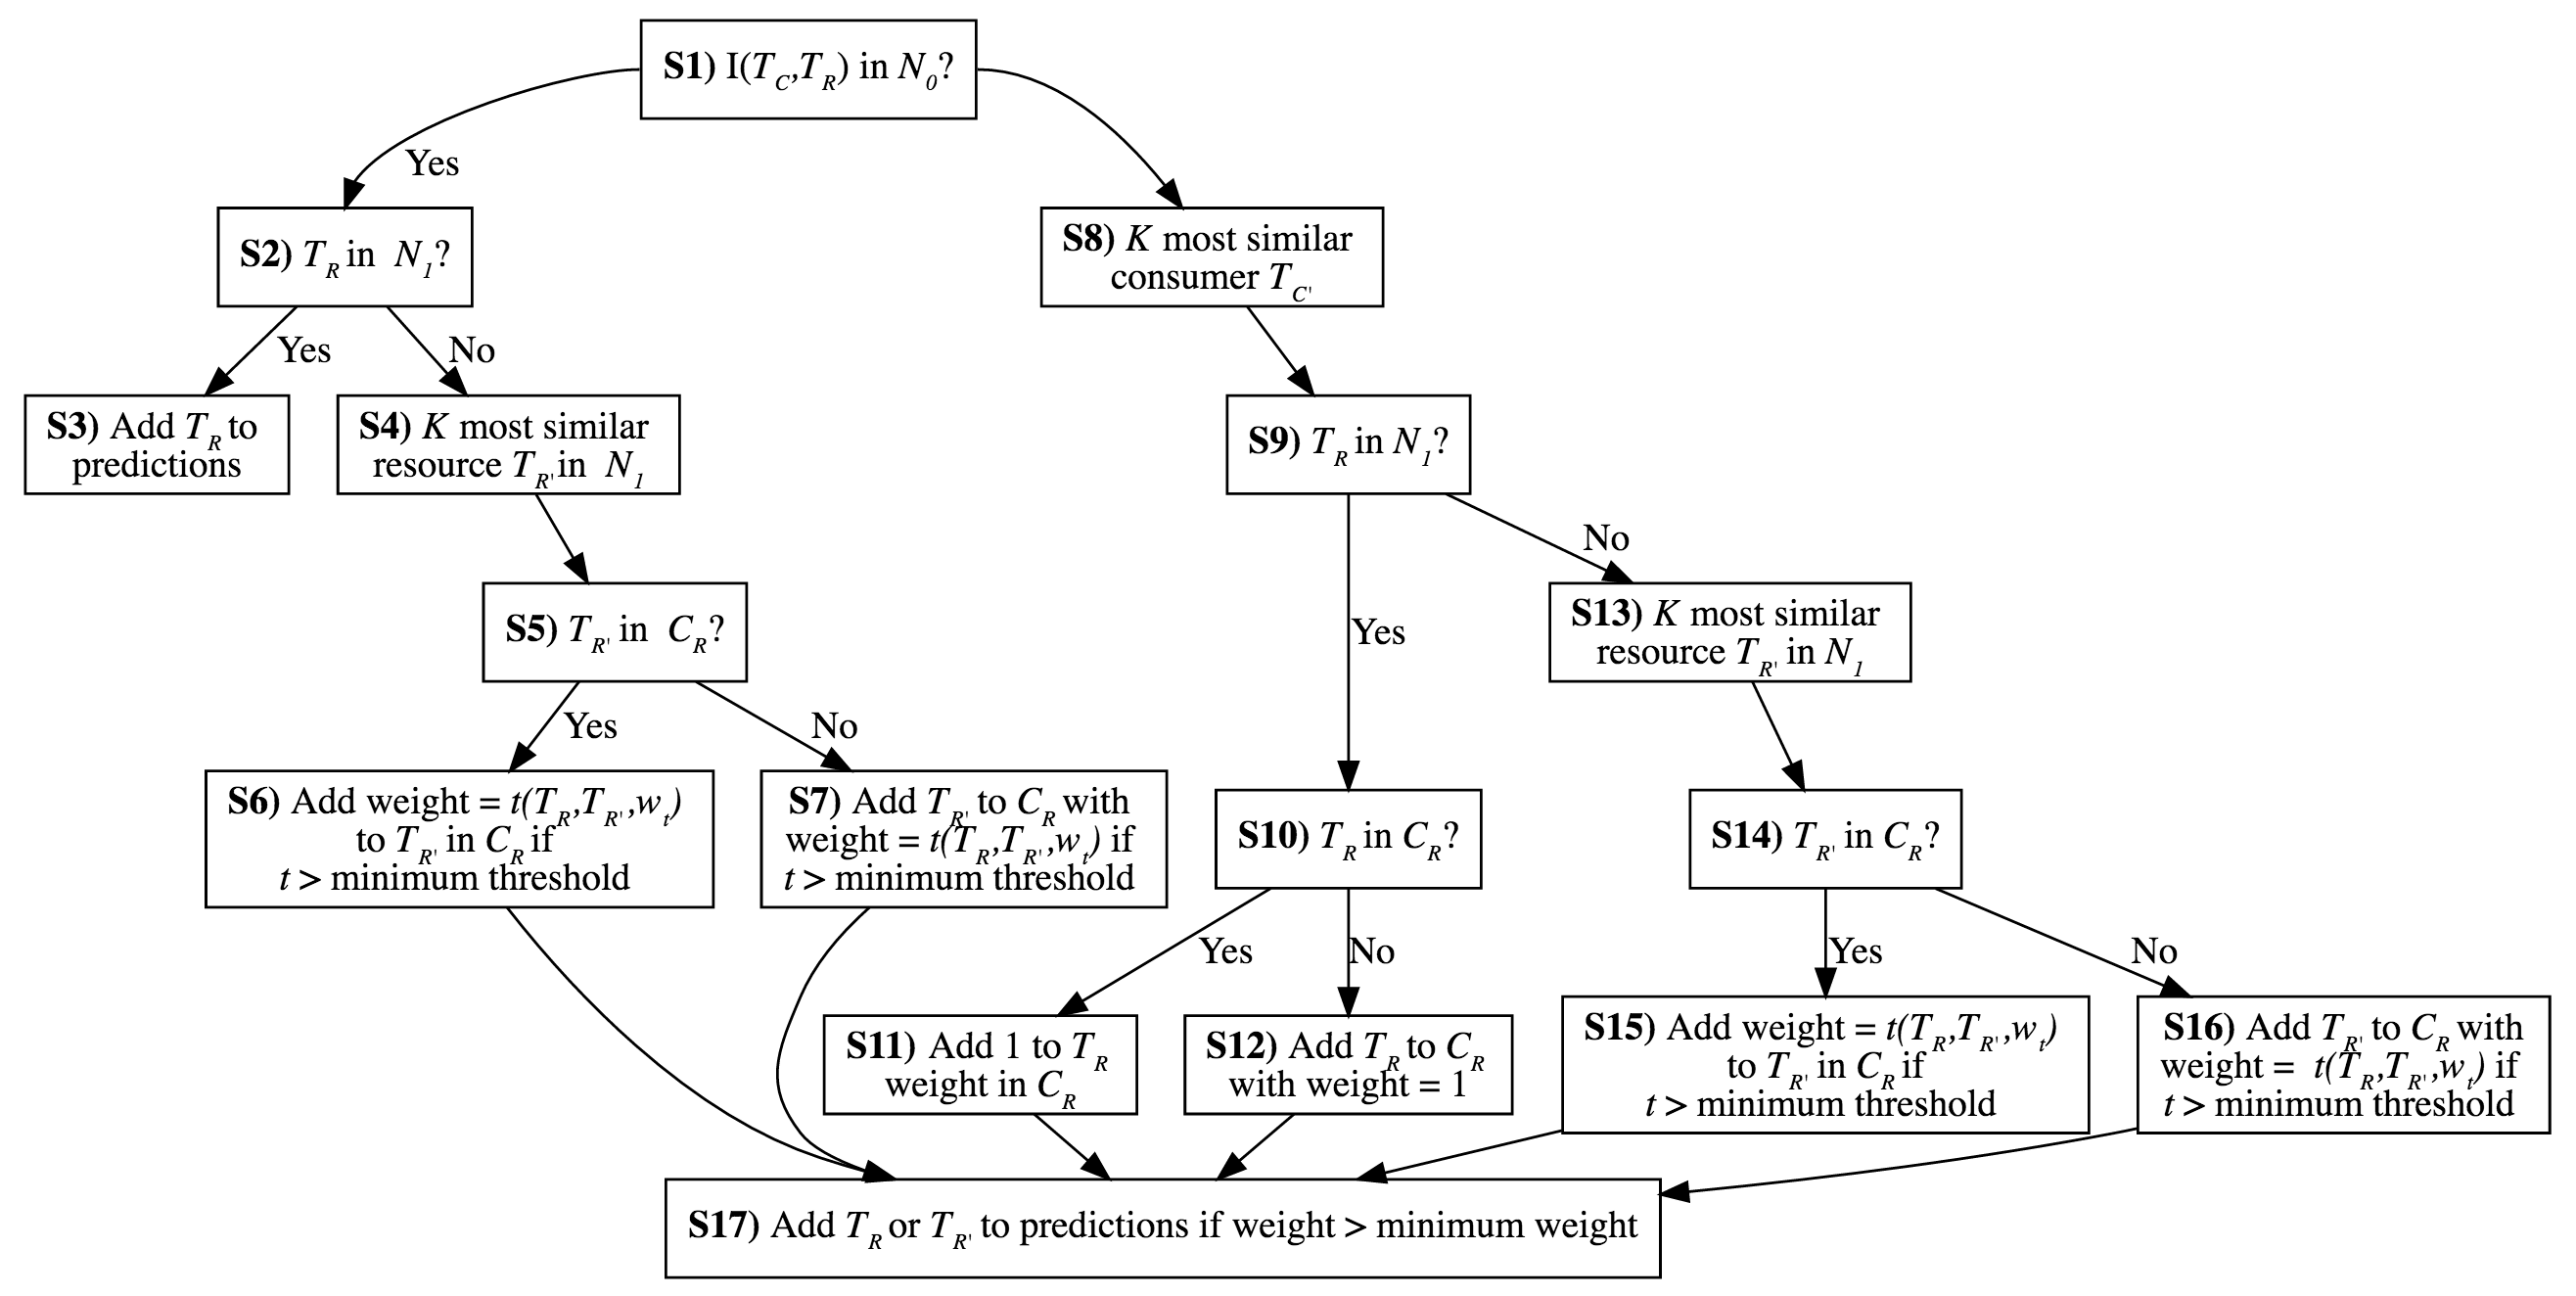
\includegraphics[width=\textwidth]{./chapitre3/figures/Decision_Diagram.png}
      \caption{Description of 17 logical steps (S1-S17) used by the algorithm to suggest a list of candidate resources ($C_R$) for each consumer taxa ($T_C$) in a set of $N_1$ for which interactions are predicted, using a set of taxa $N_0$ with empirically described interactions. Interactions between consumer and resource taxa are denoted as I($T_C$,$T_R$). $K$ is the number of most similar neighbours selected for the KNN algorithm; $t$ stands for tanimoto in equation 1; $w_t$ is the weight given to sets of resources and consumers in equation 2; the minimum threshold is a value setting the minimal similarity value accepted for taxa to be considered as close neighbours in the KNN algorithm; the weight is the value added to a candidate resource each time it is added to $C_R$; the minimum weight is the minimal weight value accepted for candidate resources to be selected as predicted sources in the algorithm.}
      \label{fig:decision_diag}
\end{figure}

% Figure 2
\newpage
    \begin{figure}[h]
      \centering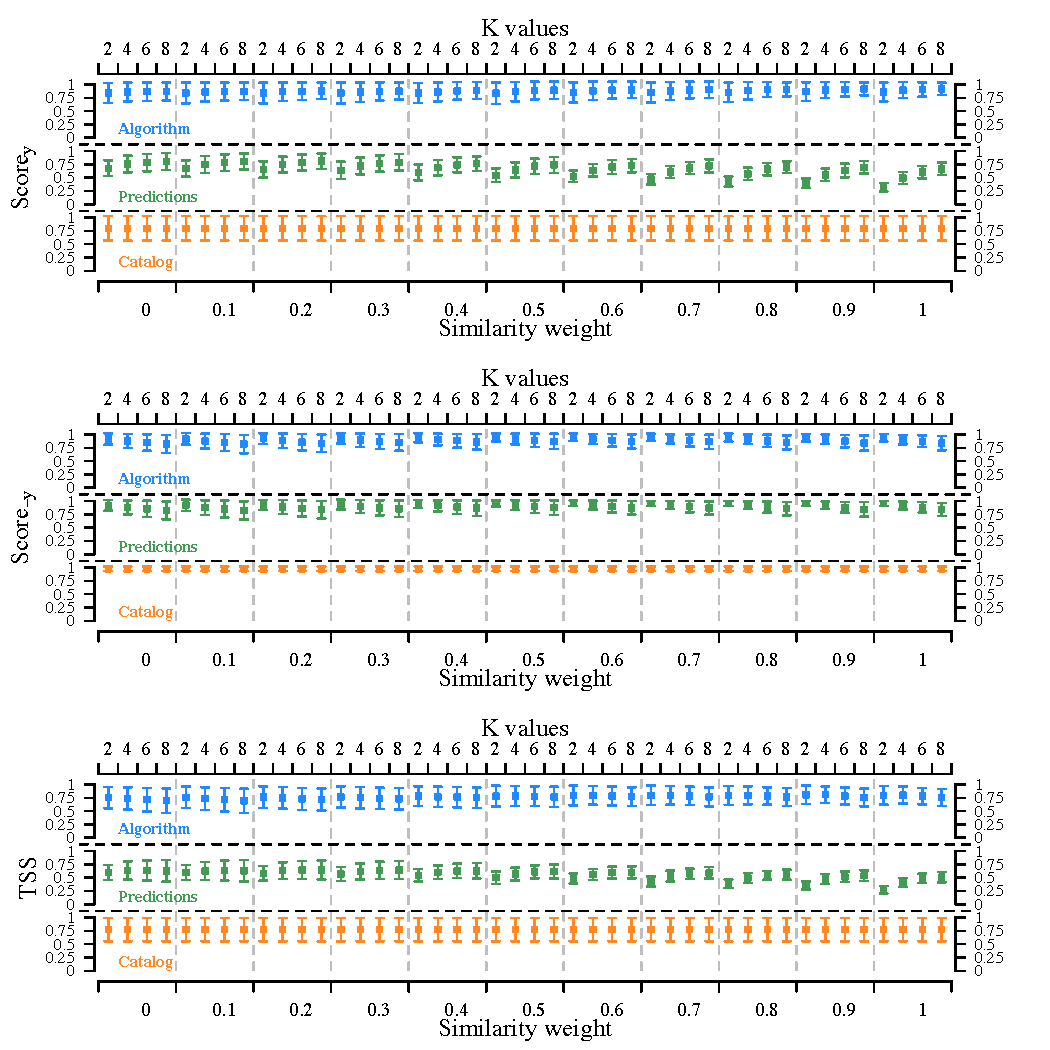
\includegraphics[width=\textwidth, height=12cm]{./chapitre3/figures/multiple_parameters2.pdf}
      \caption{Representation of the three statistics ($i.e.$ $Score_y$, $Score_{\neg y}$ and TSS) used to evaluate the accuracy of the algorithm as a function of $K$ values tested ($i.e.$ 2, 4, 6 and 8 most similar seighbours, top $x$-axis) and weight for taxonomy (bottom $x$-axis), which varies between 0 and 1. A weight of 0 means that similarity is measured only using set of resources/consumers for each taxa, while a weight of 1 means that similarity is based solely on taxonomy. For each statistic, the topmost panel presents prediction accuracy for the complete algorithm, the middle panel corresponds to predictions made through the predictive portion of the algorithm (Steps S4-S16; Figure \ref{fig:decision_diag}) and the bottom panal presents the catalogue contribution for the algorithm (Steps S1-S3; Figure \ref{fig:decision_diag}). Note that the sum of the predictive and catalogue contributions can be over 100\% as there is overlap between predictions made through both. The 7 datasets used for this analysis contained over 50 taxa \citep{christian1999, link2002, brose2005, thompson2004, barnes2008, kortsch2015}}.
      \label{fig:multi_param}
    \end{figure}

% Figure 3
\newpage
    \begin{figure}[h]
      \centering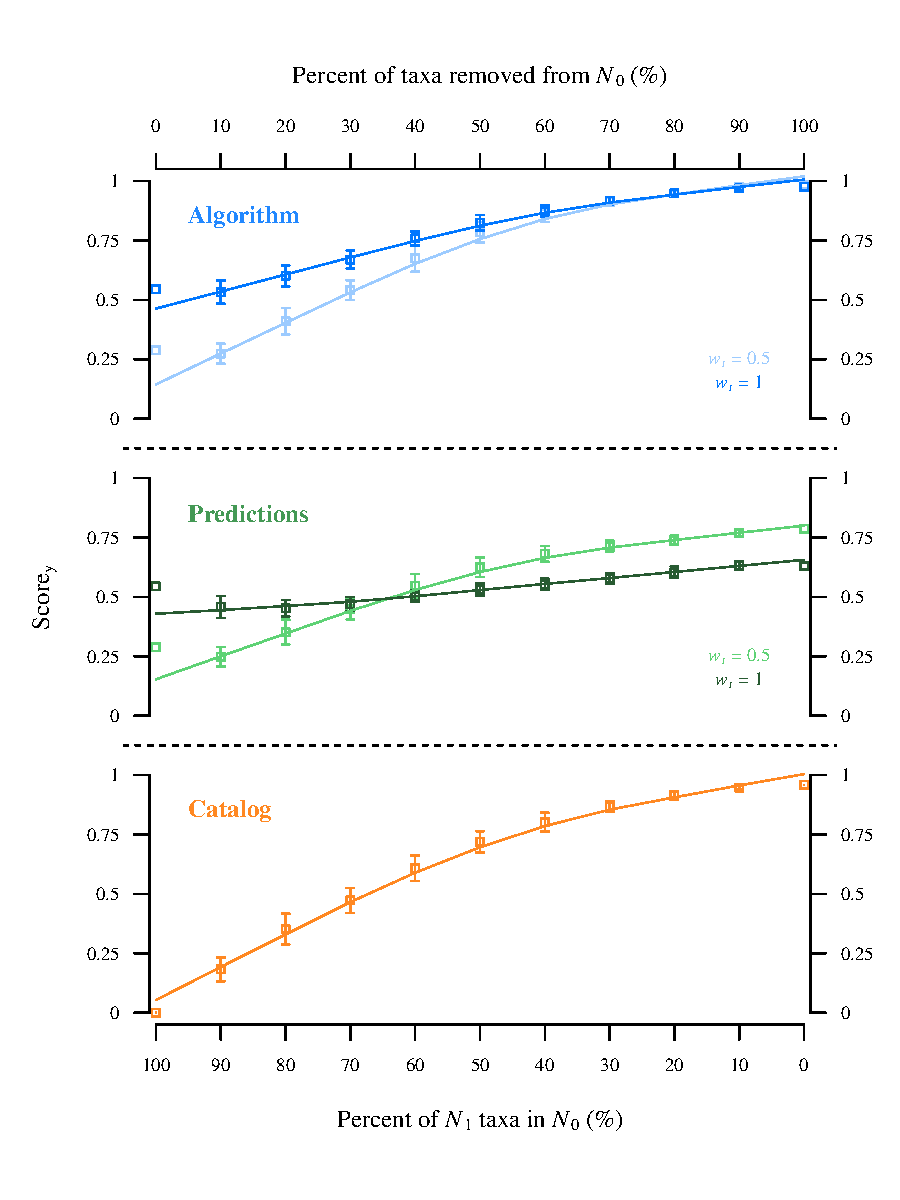
\includegraphics[height=35em]{./chapitre3/figures/catalog_predictions3.pdf}
      % \caption{Caption on next page.}
      \caption{Representation of $Score_y$ as a function of catalogue comprehensiveness, $i.e.$ the amount of information on sets of consumer and resources available in the catalogue. The sensitivity of the algorithm to data accuracy was evaluation with the arctic food web from \citet{kortsch2015}. This food web was highly detailed taxonomically. Once removed from the catalogue, almost 100\% of its taxa still had information available on sets of consumers and resources, which necessary for testing the impact of catalogue comprehensiveness on prediction accuracy. A random percentage of data available in the catalogue for taxa in the food web ($i.e.$ 0 to 100\%) was iteratively removed ($n$ = 50 randomizations) before generating new predictions with the algorithm. $w_t$ values of 0.5 and 1 were evaluated to verify the usefulness of taxonomy in supporting predictive accuracy. The topmost panel presents prediction accuracy for the complete algorithm, the middle panel corresponds to predictions made through the predictive portion of the algorithm (Steps S4-S16; Figure \ref{fig:decision_diag}) and the bottom panel presents the catalogue contribution for the algorithm (Steps S1-S3; Figure \ref{fig:decision_diag}). Note that the sum of the predictive and catalogue contributions can be over 100\% as there is overlap between predictions made through both.}
      \label{fig:catalog_pred}
    \end{figure}

% Figure 4
\newpage
    \begin{figure}[h!]
      \centering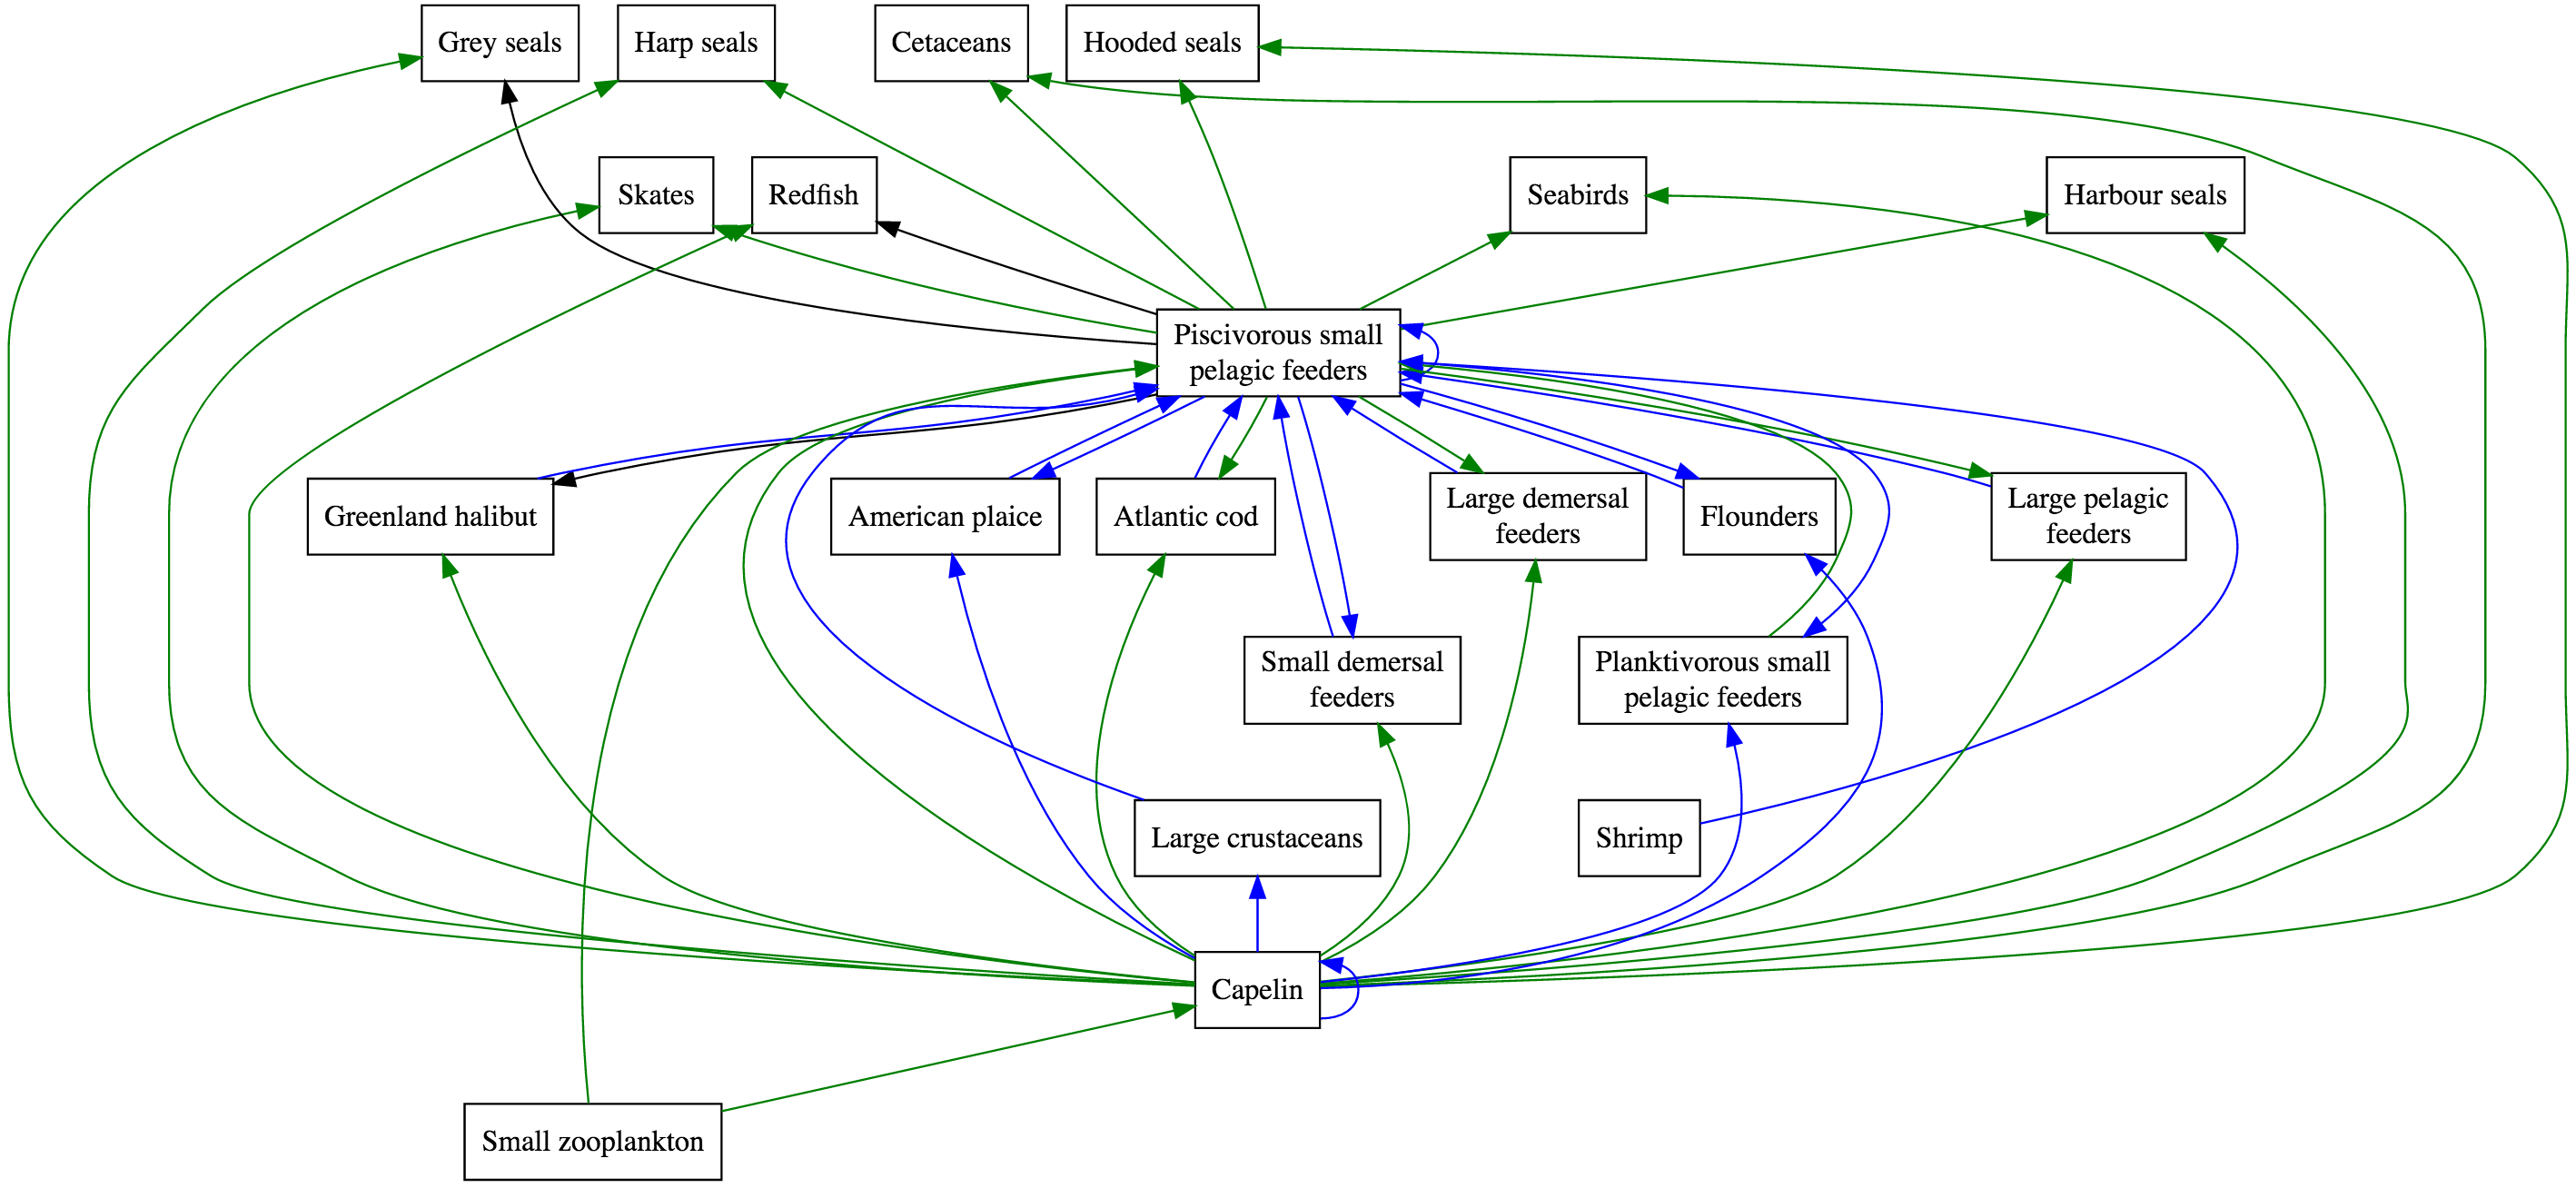
\includegraphics[width=\textwidth]{./chapitre3/figures/SGSL.png}
      \caption{Example of predicted interactions with the network of the southern Gulf of St. Lawrence \citep{savenkoff2004}, centered around the interactions of the capelin (\textit{Mallotus villosus}) and piscivorous small pelagic feeders (\textit{e.g. Scomber scombrus $and$ Illex illecebrosus}). Edge with colors green were both predicted and observed (26), black were observed only (3) and blue were predicted only (19). Arrows are pointed towards consumers.}
      \label{fig:SGSL}
    \end{figure}

\input{./chapitre4/chap4.tex}
\chapter{TITRE CHAPITRE 5}
\label{chap5}

\section{Résumé en français du deuxième article}

\subsection{Contexte scientifique}

\subsection{Publication associée}

\subsection{Traduction du résumé de l'article publié}
\hypertarget{introduction}{%
\subsection{Introduction}\label{introduction}}

\hypertarget{mat-meth}{%
\subsection{Mat \& Meth}\label{mat-meth}}


\cleardoublepage


\conclusion
\selectlanguage{french}
\input{./conclusion/conclu.tex}
\cleardoublepage




% ----------------------------------------------------------------------%
% 4 - Appendices de la thèse.                                           %
% ----------------------------------------------------------------------%


%\selectlanguage{english}
\appendice{Comment la biodiversité s'installe en territoires isolés}
\label{annI}
\addtocounter{chapter}{1}
\setcounter{equation}{0}


\section{Présenter son annexe}

C'est l'annexe 1


\section{Mega cool}

%\selectlanguage{english}
\appendice{Thinking outside the box - predicting biotic interactions in data-poor environments - Supplementary information}
\label{annII}
\addtocounter{chapter}{1}
\setcounter{equation}{0}

\begin{table}[h!]
    \centering
    \small
    \newcolumntype{b}{>{\hsize=.8\hsize}X}
    \newcolumntype{s}{>{\hsize=.2\hsize}X}
    \begin{tabularx}{1\textwidth}{|s|b|}
        \hline
        Functional group name   & Functional group main taxa composition    \\
        \hline \hline
        Cetaceans                          & $Balaenoptera$ $physalus$, $B.$ $acutorostrata$, $Megaptera$ $novaeangliae$, $Phocoena$ $phocoena$, $Lagenorhynchus$ $acutus$, $L.$ $albirostris$  \\
        \hline
        Harp seals                         & $Pagophilus$ $groenlandicus$   \\
        \hline
        Hooded seals                       & $Cystophora$ $cristata$    \\
        \hline
        Grey seals                         & $Halichoerus$ $grypus$ \\
        \hline
        Harbour seals                      & $Phoca$ $vitulina$ \\
        \hline
        Seabirds                           & $Phalacrocorax$ $carbo$, $P.$ $auritus$, $Larus$ $delawarensis$, $L.$ $argentatus$, $L.$ $marinus$, $Sterna$ $hirundo$, $S.$ $paradisaea$, $Cepphus$ $grylle$, $Oceanodroma$ $leucorhoa$, $Morus$ $bassanus$, $Rissa$ $tridactyla$, $Uria$ $aalge$, $Alca$ $torda$, $Fratercula$ $arctica$ \\
        \hline
        Atlantic cod                       & $Gadus$ $morhua$   \\
        \hline
        Greenland halibut                  & $Reinhardtius$ $hippoglossoides$   \\
        \hline
        American plaice                    & $Hippoglossoides$ $platessoides$   \\
        \hline
        Flounders                          & $Limanda$ $ferruginea$, $Glyptocephalus$ $cynoglossus$, $Pseudopleuronectes$ $americanus$  \\
        \hline
        Skates                             & $Amblyraja$ $radiata$, $Malacoraja$ $senta$, $Leucoraja$ $ocellata$    \\
        \hline
        Redfish                            & $Sebastes$ $mentella$, $S.$ $fasciatus$    \\
        \hline
        Large demersal feeders             & $Urophycis$ $tenuis$, $Melanogrammus$ $aeglefinus$, $Centroscyllium$ $fabricii$, $Anarhichas sp.$, $Cyclopterus$ $lumpus$, $Lycodes sp.$, Macrouridae, Zoarcidae, $Lophius$ $americanus$, $Hippoglossus$ $hippoglossus$    \\
        \hline
        Small demersal feeders             & $Myoxocephalus sp.$, $Tautogolabrus$ $adspersus$, $Zoarces americanus$, large demersal juveniles   \\
        \hline
        Capelin                            & $Mallotus$ $villosus$  \\
        \hline
        Large pelagic feeders              & $Squalus$ $acanthias$, $Pollachius$ $virens$, $Merluccius$ $bilinearis$, $Cetorhinus$ $maximus$    \\
        \hline
        Piscivorous small pelagic feeders  & $Scomber$ $scombrus$, $Illex$ $illecebrosus$, piscivorous myctophids and other mesopelagics, piscivorous large pelagic juveniles   \\
        \hline
        Planktivorous small pelagic feeders& $Clupea$ $harengus$ $harengus$, $Scomberesox$ $saurus$, $Gonatus sp.$, planktivorous myctiphids and other mesopelagics, planktivorous large pelagic juveniles  \\
        \hline
        Shrimp                             & $Argis$ $dentata$, $Eualus$ $macilentus$, $E.$ $gaimardi$, $Pandalus$ $montagui$   \\
        \hline
        Large crustaceans                  & $Chionoecetes$ $opilio$, $Hyas sp.$    \\
        \hline
        Echinoderms                        & $Echinarachnius$ $parma$, $Stronglyocentrotus$ $pallidus$, $Ophiura$ $robusta$ \\
        \hline
  \end{tabularx}

\end{table}

\newpage
\begin{table}[h!]
    \centering
    \small
    \newcolumntype{b}{>{\hsize=.8\hsize}X}
    \newcolumntype{s}{>{\hsize=.2\hsize}X}
    \begin{tabularx}{1\textwidth}{|s|b|}
        \hline
        Functional group name   & Functional group main taxa composition    \\
        \hline \hline
        Molluscs                           & $Mesodesma$ $deauratum$, $Cyrtodaria$ $siliqua$    \\
        \hline
        Polychates                         & $Parexogone$ $hebes$   \\
        \hline
        Small zooplankton                  & $Oithona$ $similis$, $Temora$ $longicornis$, $Pseudocalanus sp.$, $Calanus$ $finmarchicus$, tunicates, meroplankton, heterotrophic protozoa    \\
        \hline
        Phytoplankton                      & $Chaetoceros$ $affinis$, $Chaetoceros sp.$, $Leptocylindrus$ $minimus$, $Thalassiiosira$ $nordenskioldii$, $Thalassiiosira sp.$, $Fragilariopsis sp.$, other diatoms, mixture of autotrophic and mixotrophic organisms including Cryptophytes, dinoflagellates, Prasinophytes and Prymnesiophytes  \\
        \hline
  \end{tabularx}
    \caption{List of functional groups included in the dataset presented in \citet{savenkoff2004} with their taxa composition. Only taxa that were at least at the scale of the family were used to predict interactions. List adapted from \citet{savenkoff2004}.}
\end{table}

\newpage
\begin{table}[h!]
    \centering
    \begin{tabular}{|l|l|}
      \hline
        Consumer               & Resource \\
      \hline    \hline
      Skates                              & Skates    \\
      Atlantic cod                        & Skates    \\
      Hooded seals                        & Shrimp    \\
      Piscivorous small pelagic feeders   & Shrimp    \\
      Planktivorous small pelagic feeders & Phytoplankton \\
      Planktivorous small pelagic feeders & Large crustaceans \\
      Hooded seals                        & Large crustaceans \\
      Echinoderms                         & Large crustaceans \\
      Flounders                           & Large crustaceans \\
      Seabirds                            & Large crustaceans \\
      Greenland halibut                   & Large crustaceans \\
      Piscivorous small pelagic feeders   & Large crustaceans \\
      Redfish                             & Large crustaceans \\
      Planktivorous small pelagic feeders & Planktivorous small pelagic feeders   \\
      American plaice                     & Planktivorous small pelagic feeders   \\
      Echinoderms                         & Echinoderms   \\
      Large demersal feeders              & Echinoderms   \\
      Planktivorous small pelagic feeders & Atlantic cod  \\
      American plaice                     & Atlantic cod  \\
      Flounders                           & Atlantic cod  \\
      Greenland halibut                   & Atlantic cod  \\
      Piscivorous small pelagic feeders   & Atlantic cod  \\
      Cetaceans                           & American plaice   \\
      Planktivorous small pelagic feeders & American plaice   \\
      Hooded seals                        & American plaice   \\
      American plaice                     & American plaice   \\
      Flounders                           & American plaice   \\
      Harbour seals                       & American plaice   \\
      Piscivorous small pelagic feeders   & American plaice   \\
      Redfish                             & American plaice   \\
      Large pelagic feeders               & American plaice   \\
      Cetaceans                           & Flounders \\
      Planktivorous small pelagic feeders & Flounders \\
      American plaice                     & Flounders \\
      Flounders                           & Flounders \\
      Piscivorous small pelagic feeders   & Flounders \\
      Redfish                             & Flounders \\
      Large crustaceans                   & Capelin   \\
      Planktivorous small pelagic feeders & Capelin   \\
      Piscivorous small pelagic feeders   & Small demersal feeders    \\
      \hline
  \end{tabular}
\end{table}
\newpage
\begin{table}[h!]
  \centering
  \begin{tabular}{|l|l|}
      \hline
      Consumer               & Resource \\
      \hline    \hline
      Cetaceans                           & Small zooplankton \\
      Large crustaceans                   & Small zooplankton \\
      Large pelagic feeders               & Small zooplankton \\
      Large demersal feeders              & Small zooplankton \\
      Atlantic cod                        & Seabirds  \\
      Seabirds                            & Seabirds  \\
      Large demersal feeders              & Seabirds  \\
      Harbour seals                       & Harbour seals \\
      Skates                              & Greenland halibut \\
      Cetaceans                           & Greenland halibut \\
      Planktivorous small pelagic feeders & Greenland halibut \\
      Atlantic cod                        & Greenland halibut \\
      American plaice                     & Greenland halibut \\
      Flounders                           & Greenland halibut \\
      Small demersal feeders              & Greenland halibut \\
      Harbour seals                       & Greenland halibut \\
      Piscivorous small pelagic feeders   & Greenland halibut \\
      Redfish                             & Greenland halibut \\
      Large pelagic feeders               & Greenland halibut \\
      Planktivorous small pelagic feeders & Piscivorous small pelagic feeders \\
      American plaice                     & Piscivorous small pelagic feeders \\
      Flounders                           & Piscivorous small pelagic feeders \\
      Small demersal feeders              & Piscivorous small pelagic feeders \\
      Piscivorous small pelagic feeders   & Piscivorous small pelagic feeders \\
      Atlantic cod                        & Redfish   \\
      Harp seals                          & Redfish   \\
      Seabirds                            & Redfish   \\
      Redfish                             & Redfish   \\
      Large pelagic feeders               & Redfish   \\
      Skates                              & Large pelagic feeders \\
      Planktivorous small pelagic feeders & Large pelagic feeders \\
      Hooded seals                        & Large pelagic feeders \\
      Atlantic cod                        & Large pelagic feeders \\
      American plaice                     & Large pelagic feeders \\
      Flounders                           & Large pelagic feeders \\
      Small demersal feeders              & Large pelagic feeders \\
      Harp seals                          & Large pelagic feeders \\
      Seabirds                            & Large pelagic feeders \\
      Greenland halibut                   & Large pelagic feeders \\
      Piscivorous small pelagic feeders   & Large pelagic feeders \\
      \hline
    \end{tabular}
\end{table}
\newpage
\begin{table}[h!]
    \centering
    \begin{tabular}{|l|l|}
    \hline
    Consumer               & Resource \\
    \hline    \hline
    Redfish                             & Large pelagic feeders \\
    Large pelagic feeders               & Large pelagic feeders \\
    Large demersal feeders              & Large pelagic feeders \\
    Skates                              & Large demersal feeders    \\
    Cetaceans                           & Large demersal feeders    \\
    Planktivorous small pelagic feeders & Large demersal feeders    \\
    Atlantic cod                        & Large demersal feeders    \\
    American plaice                     & Large demersal feeders    \\
    Flounders                           & Large demersal feeders    \\
    Small demersal feeders              & Large demersal feeders    \\
    Seabirds                            & Large demersal feeders    \\
    Greenland halibut                   & Large demersal feeders    \\
    Piscivorous small pelagic feeders   & Large demersal feeders    \\
    Redfish                             & Large demersal feeders    \\
    Large pelagic feeders               & Large demersal feeders    \\
    Large demersal feeders              & Large demersal feeders    \\
    \hline
\end{tabular}
    \caption{List of functional groups for which interactions were predicted by the algorithm, but not observed in \citet{savenkoff2004} ($b$).}
\end{table}

\newpage
\begin{table}[h!]
  \centering
  \begin{tabular}{|l|l|}
    \hline
      Consumer               & Resource \\
    \hline  \hline
    Grey seals             & Skates \\
    Seabirds               & Skates \\
    Harbour seals          & Skates \\
    Cetaceans              & Shrimp \\
    Shrimp                 & Phytoplankton  \\
    Mollusks               & Phytoplankton  \\
    Polychaetes            & Phytoplankton  \\
    Grey seals             & Large crustaceans  \\
    Flounders              & Planktivorous small pelagic feeders    \\
    Flounders              & Echinoderms    \\
    Small demersal feeders & Echinoderms    \\
    Grey seals             & American plaice    \\
    Hooded seals           & Flounders  \\
    Harp seals             & Flounders  \\
    Skates                 & Mollusks   \\
    Large crustaceans      & Mollusks   \\
    Atlantic cod           & Mollusks   \\
    American plaice        & Mollusks   \\
    Flounders              & Mollusks   \\
    Small demersal feeders & Mollusks   \\
    Harbour seals          & Mollusks   \\
    Seabirds               & Small zooplankton  \\
    Skates                 & Polychaetes    \\
    Shrimp                 & Polychaetes    \\
    Large crustaceans      & Polychaetes    \\
    Atlantic cod           & Polychaetes    \\
    American plaice        & Polychaetes    \\
    Flounders              & Polychaetes    \\
    Small demersal feeders & Polychaetes    \\
    Polychaetes            & Polychaetes    \\
    Large pelagic feeders  & Polychaetes    \\
    Large demersal feeders & Polychaetes    \\
    Grey seals             & Piscivorous small pelagic feeders  \\
    Greenland halibut      & Piscivorous small pelagic feeders  \\
    Redfish                & Piscivorous small pelagic feeders  \\
    \hline
  \end{tabular}
  \caption{List of functional groups for which observed interactions in \citet{savenkoff2004} were not predicted by the algorithm ($c$).}
\end{table}

%\selectlanguage{english}
\appendice{Thinking outside the box - predicting biotic interactions in data-poor environments - Supplementary information}
\label{annIII}
\addtocounter{chapter}{1}
\setcounter{equation}{0}

\begin{table}[h!]
    \centering
    \small
    \newcolumntype{b}{>{\hsize=.8\hsize}X}
    \newcolumntype{s}{>{\hsize=.2\hsize}X}
    \begin{tabularx}{1\textwidth}{|s|b|}
        \hline
        Functional group name   & Functional group main taxa composition    \\
        \hline \hline
        Cetaceans                          & $Balaenoptera$ $physalus$, $B.$ $acutorostrata$, $Megaptera$ $novaeangliae$, $Phocoena$ $phocoena$, $Lagenorhynchus$ $acutus$, $L.$ $albirostris$  \\
        \hline
        Harp seals                         & $Pagophilus$ $groenlandicus$   \\
        \hline
        Hooded seals                       & $Cystophora$ $cristata$    \\
        \hline
        Grey seals                         & $Halichoerus$ $grypus$ \\
        \hline
        Harbour seals                      & $Phoca$ $vitulina$ \\
        \hline
        Seabirds                           & $Phalacrocorax$ $carbo$, $P.$ $auritus$, $Larus$ $delawarensis$, $L.$ $argentatus$, $L.$ $marinus$, $Sterna$ $hirundo$, $S.$ $paradisaea$, $Cepphus$ $grylle$, $Oceanodroma$ $leucorhoa$, $Morus$ $bassanus$, $Rissa$ $tridactyla$, $Uria$ $aalge$, $Alca$ $torda$, $Fratercula$ $arctica$ \\
        \hline
        Atlantic cod                       & $Gadus$ $morhua$   \\
        \hline
        Greenland halibut                  & $Reinhardtius$ $hippoglossoides$   \\
        \hline
        American plaice                    & $Hippoglossoides$ $platessoides$   \\
        \hline
        Flounders                          & $Limanda$ $ferruginea$, $Glyptocephalus$ $cynoglossus$, $Pseudopleuronectes$ $americanus$  \\
        \hline
        Skates                             & $Amblyraja$ $radiata$, $Malacoraja$ $senta$, $Leucoraja$ $ocellata$    \\
        \hline
        Redfish                            & $Sebastes$ $mentella$, $S.$ $fasciatus$    \\
        \hline
        Large demersal feeders             & $Urophycis$ $tenuis$, $Melanogrammus$ $aeglefinus$, $Centroscyllium$ $fabricii$, $Anarhichas sp.$, $Cyclopterus$ $lumpus$, $Lycodes sp.$, Macrouridae, Zoarcidae, $Lophius$ $americanus$, $Hippoglossus$ $hippoglossus$    \\
        \hline
        Small demersal feeders             & $Myoxocephalus sp.$, $Tautogolabrus$ $adspersus$, $Zoarces americanus$, large demersal juveniles   \\
        \hline
        Capelin                            & $Mallotus$ $villosus$  \\
        \hline
        Large pelagic feeders              & $Squalus$ $acanthias$, $Pollachius$ $virens$, $Merluccius$ $bilinearis$, $Cetorhinus$ $maximus$    \\
        \hline
        Piscivorous small pelagic feeders  & $Scomber$ $scombrus$, $Illex$ $illecebrosus$, piscivorous myctophids and other mesopelagics, piscivorous large pelagic juveniles   \\
        \hline
        Planktivorous small pelagic feeders& $Clupea$ $harengus$ $harengus$, $Scomberesox$ $saurus$, $Gonatus sp.$, planktivorous myctiphids and other mesopelagics, planktivorous large pelagic juveniles  \\
        \hline
        Shrimp                             & $Argis$ $dentata$, $Eualus$ $macilentus$, $E.$ $gaimardi$, $Pandalus$ $montagui$   \\
        \hline
        Large crustaceans                  & $Chionoecetes$ $opilio$, $Hyas sp.$    \\
        \hline
        Echinoderms                        & $Echinarachnius$ $parma$, $Stronglyocentrotus$ $pallidus$, $Ophiura$ $robusta$ \\
        \hline
  \end{tabularx}

\end{table}

\newpage
\begin{table}[h!]
    \centering
    \small
    \newcolumntype{b}{>{\hsize=.8\hsize}X}
    \newcolumntype{s}{>{\hsize=.2\hsize}X}
    \begin{tabularx}{1\textwidth}{|s|b|}
        \hline
        Functional group name   & Functional group main taxa composition    \\
        \hline \hline
        Molluscs                           & $Mesodesma$ $deauratum$, $Cyrtodaria$ $siliqua$    \\
        \hline
        Polychates                         & $Parexogone$ $hebes$   \\
        \hline
        Small zooplankton                  & $Oithona$ $similis$, $Temora$ $longicornis$, $Pseudocalanus sp.$, $Calanus$ $finmarchicus$, tunicates, meroplankton, heterotrophic protozoa    \\
        \hline
        Phytoplankton                      & $Chaetoceros$ $affinis$, $Chaetoceros sp.$, $Leptocylindrus$ $minimus$, $Thalassiiosira$ $nordenskioldii$, $Thalassiiosira sp.$, $Fragilariopsis sp.$, other diatoms, mixture of autotrophic and mixotrophic organisms including Cryptophytes, dinoflagellates, Prasinophytes and Prymnesiophytes  \\
        \hline
  \end{tabularx}
    \caption{List of functional groups included in the dataset presented in \citet{Savenkoff2004} with their taxa composition. Only taxa that were at least at the scale of the family were used to predict interactions. List adapted from \citet{Savenkoff2004}.}
\end{table}

\newpage
\begin{table}[h!]
    \centering
    \begin{tabular}{|l|l|}
      \hline
        Consumer               & Resource \\
      \hline    \hline
      Skates                              & Skates    \\
      Atlantic cod                        & Skates    \\
      Hooded seals                        & Shrimp    \\
      Piscivorous small pelagic feeders   & Shrimp    \\
      Planktivorous small pelagic feeders & Phytoplankton \\
      Planktivorous small pelagic feeders & Large crustaceans \\
      Hooded seals                        & Large crustaceans \\
      Echinoderms                         & Large crustaceans \\
      Flounders                           & Large crustaceans \\
      Seabirds                            & Large crustaceans \\
      Greenland halibut                   & Large crustaceans \\
      Piscivorous small pelagic feeders   & Large crustaceans \\
      Redfish                             & Large crustaceans \\
      Planktivorous small pelagic feeders & Planktivorous small pelagic feeders   \\
      American plaice                     & Planktivorous small pelagic feeders   \\
      Echinoderms                         & Echinoderms   \\
      Large demersal feeders              & Echinoderms   \\
      Planktivorous small pelagic feeders & Atlantic cod  \\
      American plaice                     & Atlantic cod  \\
      Flounders                           & Atlantic cod  \\
      Greenland halibut                   & Atlantic cod  \\
      Piscivorous small pelagic feeders   & Atlantic cod  \\
      Cetaceans                           & American plaice   \\
      Planktivorous small pelagic feeders & American plaice   \\
      Hooded seals                        & American plaice   \\
      American plaice                     & American plaice   \\
      Flounders                           & American plaice   \\
      Harbour seals                       & American plaice   \\
      Piscivorous small pelagic feeders   & American plaice   \\
      Redfish                             & American plaice   \\
      Large pelagic feeders               & American plaice   \\
      Cetaceans                           & Flounders \\
      Planktivorous small pelagic feeders & Flounders \\
      American plaice                     & Flounders \\
      Flounders                           & Flounders \\
      Piscivorous small pelagic feeders   & Flounders \\
      Redfish                             & Flounders \\
      Large crustaceans                   & Capelin   \\
      Planktivorous small pelagic feeders & Capelin   \\
      Piscivorous small pelagic feeders   & Small demersal feeders    \\
      \hline
  \end{tabular}
\end{table}
\newpage
\begin{table}[h!]
  \centering
  \begin{tabular}{|l|l|}
      \hline
      Consumer               & Resource \\
      \hline    \hline
      Cetaceans                           & Small zooplankton \\
      Large crustaceans                   & Small zooplankton \\
      Large pelagic feeders               & Small zooplankton \\
      Large demersal feeders              & Small zooplankton \\
      Atlantic cod                        & Seabirds  \\
      Seabirds                            & Seabirds  \\
      Large demersal feeders              & Seabirds  \\
      Harbour seals                       & Harbour seals \\
      Skates                              & Greenland halibut \\
      Cetaceans                           & Greenland halibut \\
      Planktivorous small pelagic feeders & Greenland halibut \\
      Atlantic cod                        & Greenland halibut \\
      American plaice                     & Greenland halibut \\
      Flounders                           & Greenland halibut \\
      Small demersal feeders              & Greenland halibut \\
      Harbour seals                       & Greenland halibut \\
      Piscivorous small pelagic feeders   & Greenland halibut \\
      Redfish                             & Greenland halibut \\
      Large pelagic feeders               & Greenland halibut \\
      Planktivorous small pelagic feeders & Piscivorous small pelagic feeders \\
      American plaice                     & Piscivorous small pelagic feeders \\
      Flounders                           & Piscivorous small pelagic feeders \\
      Small demersal feeders              & Piscivorous small pelagic feeders \\
      Piscivorous small pelagic feeders   & Piscivorous small pelagic feeders \\
      Atlantic cod                        & Redfish   \\
      Harp seals                          & Redfish   \\
      Seabirds                            & Redfish   \\
      Redfish                             & Redfish   \\
      Large pelagic feeders               & Redfish   \\
      Skates                              & Large pelagic feeders \\
      Planktivorous small pelagic feeders & Large pelagic feeders \\
      Hooded seals                        & Large pelagic feeders \\
      Atlantic cod                        & Large pelagic feeders \\
      American plaice                     & Large pelagic feeders \\
      Flounders                           & Large pelagic feeders \\
      Small demersal feeders              & Large pelagic feeders \\
      Harp seals                          & Large pelagic feeders \\
      Seabirds                            & Large pelagic feeders \\
      Greenland halibut                   & Large pelagic feeders \\
      Piscivorous small pelagic feeders   & Large pelagic feeders \\
      \hline
    \end{tabular}
\end{table}
\newpage
\begin{table}[h!]
    \centering
    \begin{tabular}{|l|l|}
    \hline
    Consumer               & Resource \\
    \hline    \hline
    Redfish                             & Large pelagic feeders \\
    Large pelagic feeders               & Large pelagic feeders \\
    Large demersal feeders              & Large pelagic feeders \\
    Skates                              & Large demersal feeders    \\
    Cetaceans                           & Large demersal feeders    \\
    Planktivorous small pelagic feeders & Large demersal feeders    \\
    Atlantic cod                        & Large demersal feeders    \\
    American plaice                     & Large demersal feeders    \\
    Flounders                           & Large demersal feeders    \\
    Small demersal feeders              & Large demersal feeders    \\
    Seabirds                            & Large demersal feeders    \\
    Greenland halibut                   & Large demersal feeders    \\
    Piscivorous small pelagic feeders   & Large demersal feeders    \\
    Redfish                             & Large demersal feeders    \\
    Large pelagic feeders               & Large demersal feeders    \\
    Large demersal feeders              & Large demersal feeders    \\
    \hline
\end{tabular}
    \caption{List of functional groups for which interactions were predicted by the algorithm, but not observed in \citet{Savenkoff2004} ($b$).}
\end{table}

\newpage
\begin{table}[h!]
  \centering
  \begin{tabular}{|l|l|}
    \hline
      Consumer               & Resource \\
    \hline  \hline
    Grey seals             & Skates \\
    Seabirds               & Skates \\
    Harbour seals          & Skates \\
    Cetaceans              & Shrimp \\
    Shrimp                 & Phytoplankton  \\
    Mollusks               & Phytoplankton  \\
    Polychaetes            & Phytoplankton  \\
    Grey seals             & Large crustaceans  \\
    Flounders              & Planktivorous small pelagic feeders    \\
    Flounders              & Echinoderms    \\
    Small demersal feeders & Echinoderms    \\
    Grey seals             & American plaice    \\
    Hooded seals           & Flounders  \\
    Harp seals             & Flounders  \\
    Skates                 & Mollusks   \\
    Large crustaceans      & Mollusks   \\
    Atlantic cod           & Mollusks   \\
    American plaice        & Mollusks   \\
    Flounders              & Mollusks   \\
    Small demersal feeders & Mollusks   \\
    Harbour seals          & Mollusks   \\
    Seabirds               & Small zooplankton  \\
    Skates                 & Polychaetes    \\
    Shrimp                 & Polychaetes    \\
    Large crustaceans      & Polychaetes    \\
    Atlantic cod           & Polychaetes    \\
    American plaice        & Polychaetes    \\
    Flounders              & Polychaetes    \\
    Small demersal feeders & Polychaetes    \\
    Polychaetes            & Polychaetes    \\
    Large pelagic feeders  & Polychaetes    \\
    Large demersal feeders & Polychaetes    \\
    Grey seals             & Piscivorous small pelagic feeders  \\
    Greenland halibut      & Piscivorous small pelagic feeders  \\
    Redfish                & Piscivorous small pelagic feeders  \\
    \hline
  \end{tabular}
  \caption{List of functional groups for which observed interactions in \citet{Savenkoff2004} were not predicted by the algorithm ($c$).}
\end{table}

%\input{./annexe4/annexe4.tex}




% ----------------------------------------------------------------------%
% 5 - Bibliographie.                                                    %
% ----------------------------------------------------------------------%

\selectlanguage{english}

\begin{singlespace}
  \makeatletter
  \phantomsection\addcontentsline{toc}{chapter}{\MakeUppercase{\@references}}
  \makeatother
  \bibliographystyle{apalike}
  \bibliography{mybiblio.bib} % Ici mettre le nom de la biblio, ici mylib.bib
\end{singlespace}

% \begin{singlespace}
%   \makeatletter
%   \phantomsection\addcontentsline{toc}{chapter}{\MakeUppercase{\@references}}
%   \makeatother
%   \selectlanguage{english}
%   % \bibliographystyle{elsevier-harvard.csl} % Ici éditer le style
%   \bibliography{/Users/KevCaz/Documents/library.bib} % Ici mettre le nom de la biblio, ici mylib.bib
% \end{singlespace}



% ----------------------------------------------------------------------%
% Fin du document.                                                     %
% ----------------------------------------------------------------------%

\end{document}
